% TeX eps-loader file generated by stoch_simul.m (Dynare).
% 07-May-2024 13:28:03
 
\begin{figure}[H]
\centering 
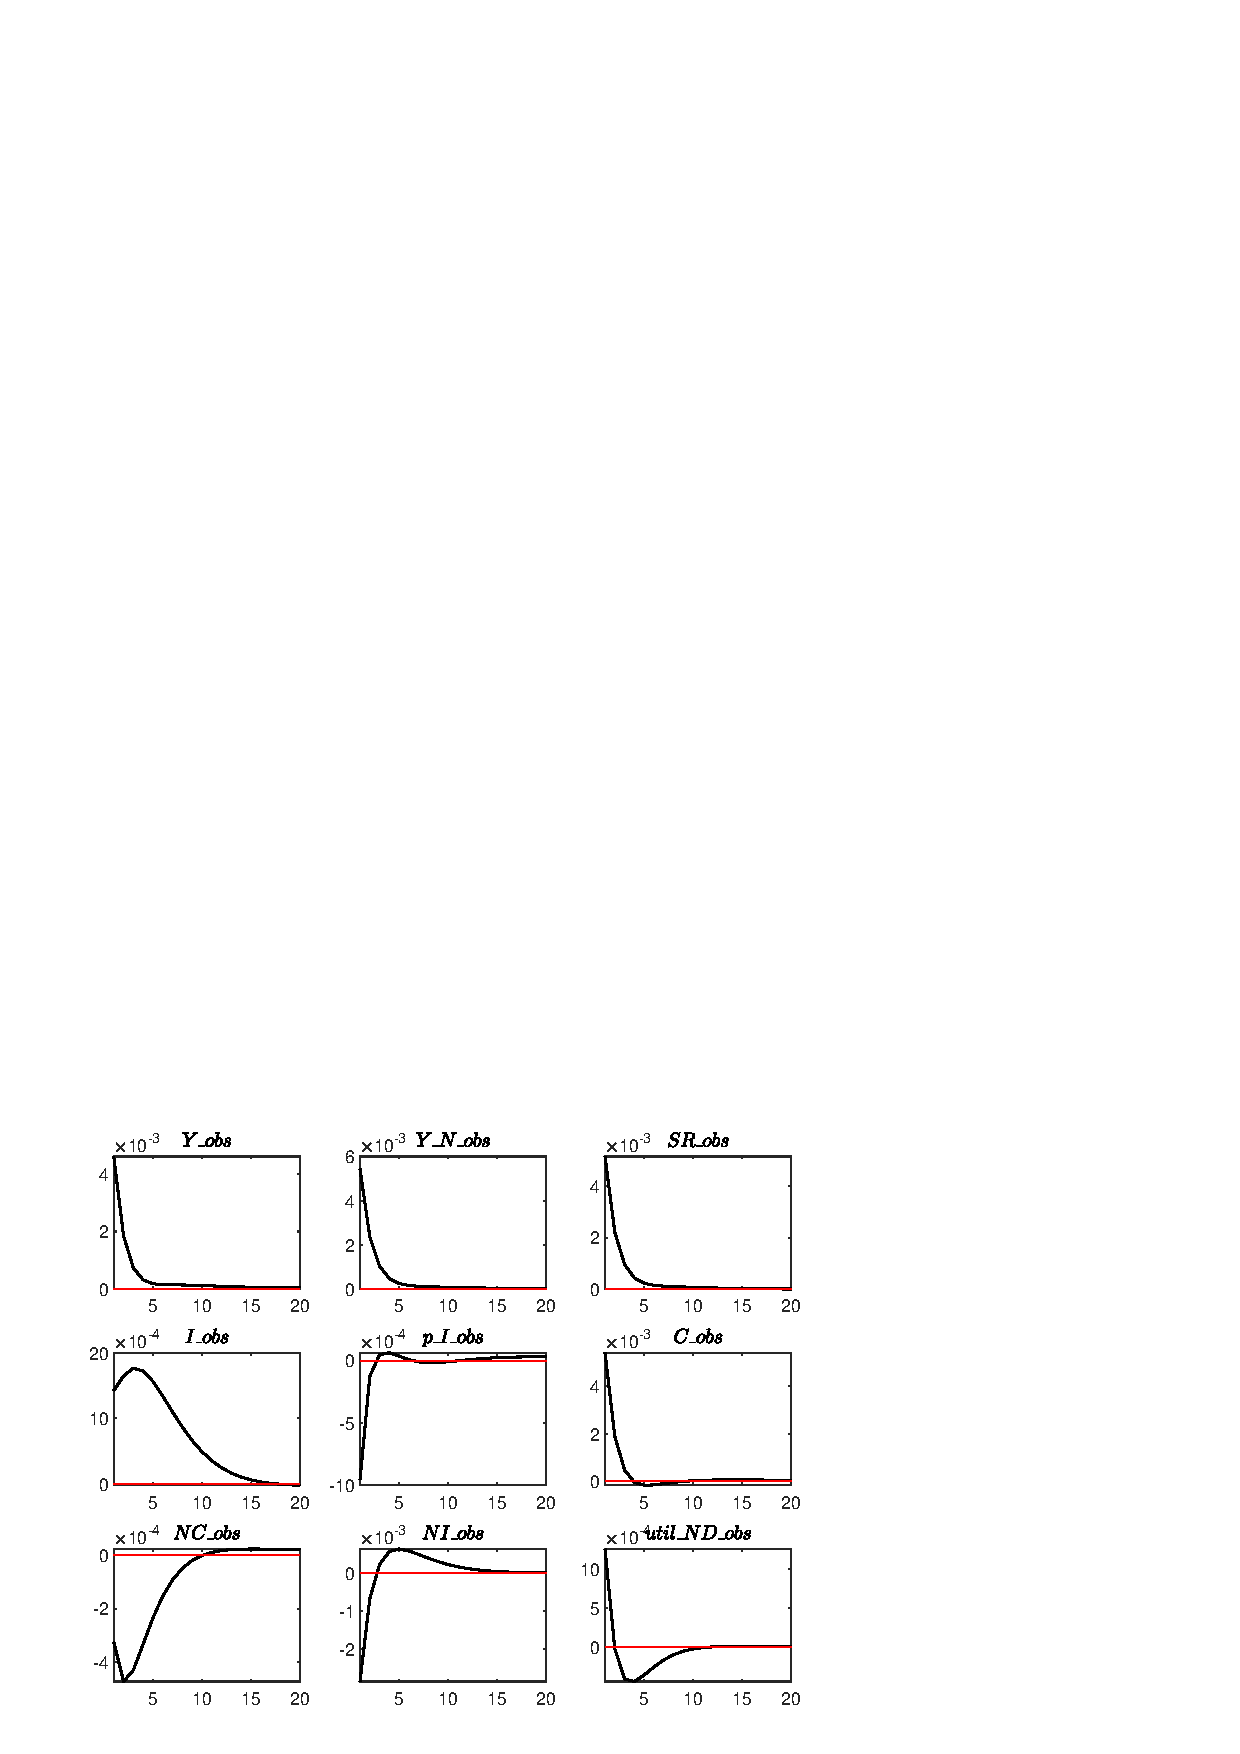
\includegraphics[width=0.80\textwidth]{BRS_sectoral/graphs/BRS_sectoral_IRF_e_g1}
\caption{Impulse response functions (orthogonalized shock to ${e_g}$).}\label{Fig:IRF:e_g:1}
\end{figure}
 
\begin{figure}[H]
\centering 
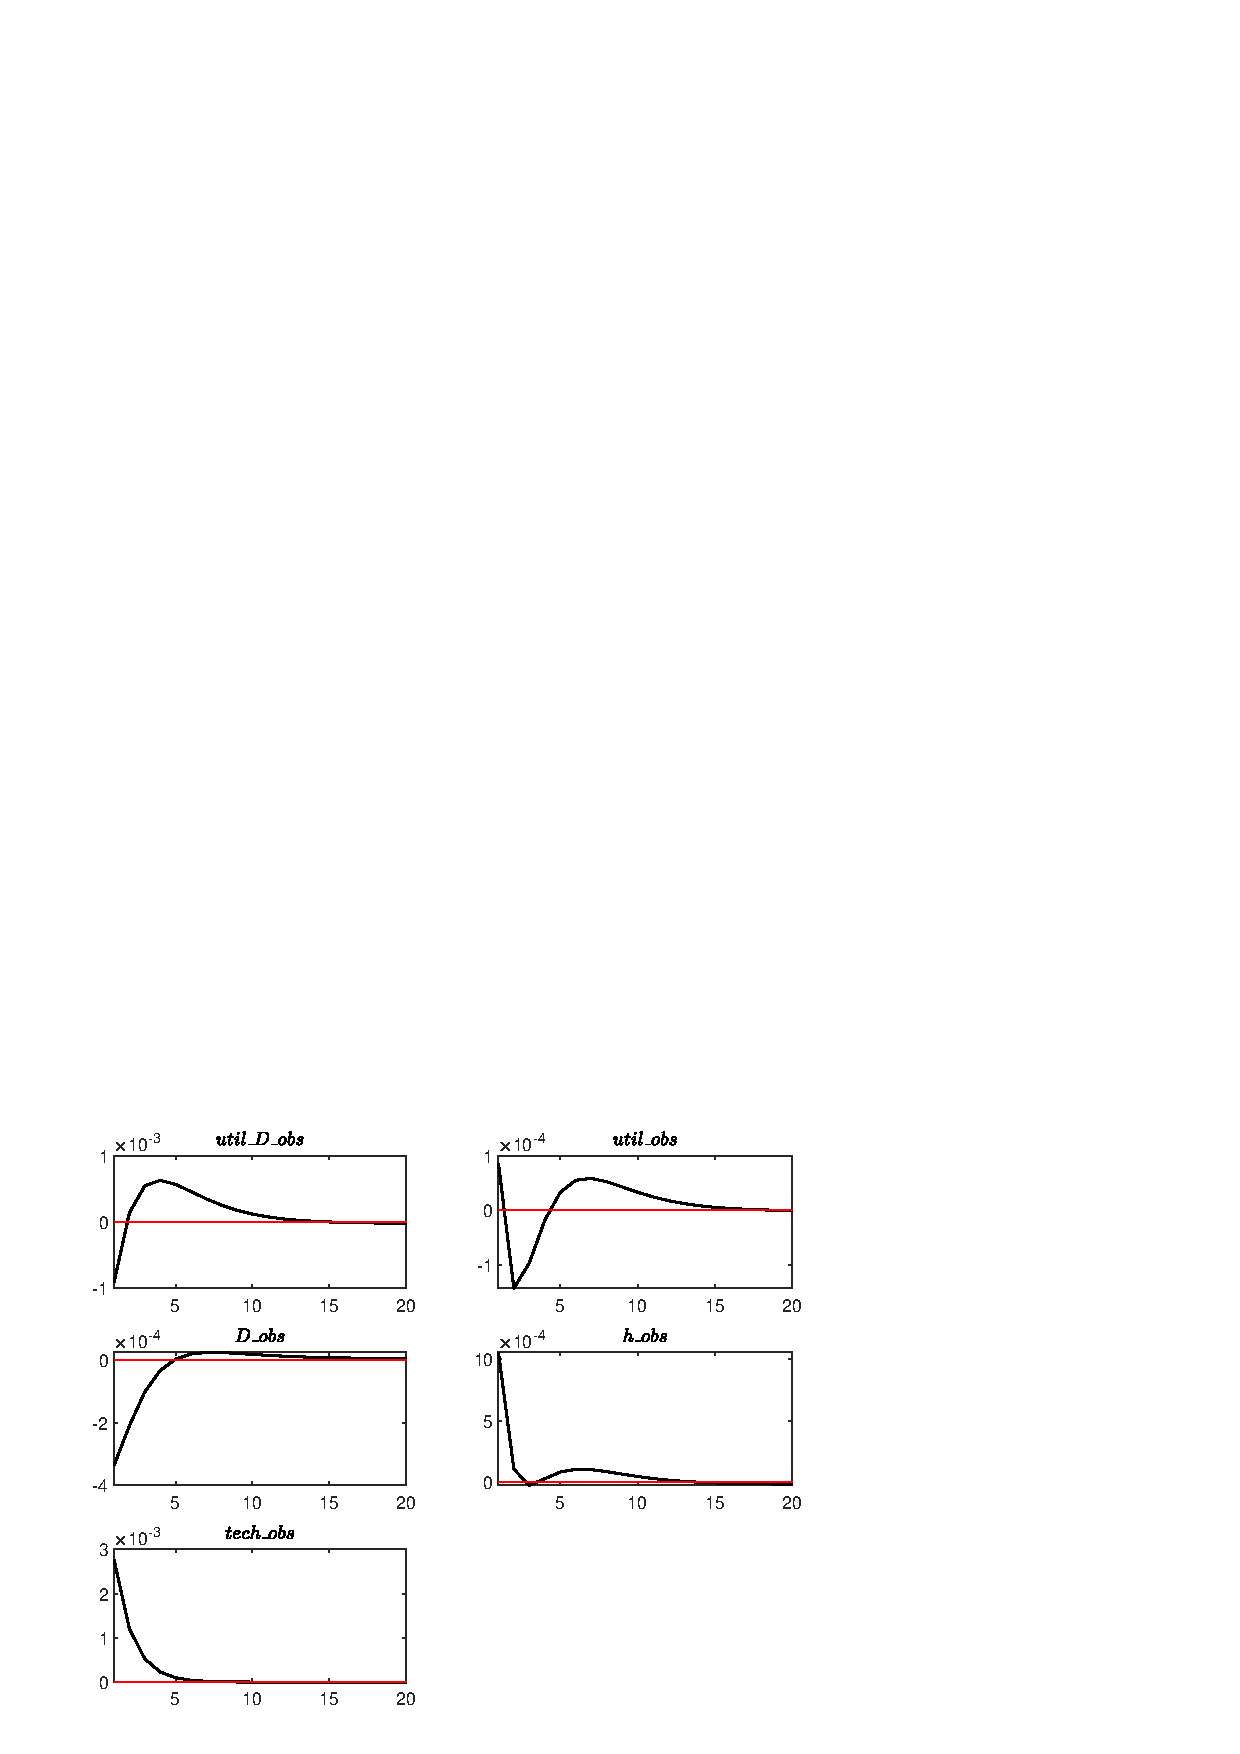
\includegraphics[width=0.80\textwidth]{BRS_sectoral/graphs/BRS_sectoral_IRF_e_g2}
\caption{Impulse response functions (orthogonalized shock to ${e_g}$).}\label{Fig:IRF:e_g:2}
\end{figure}
 
\begin{figure}[H]
\centering 
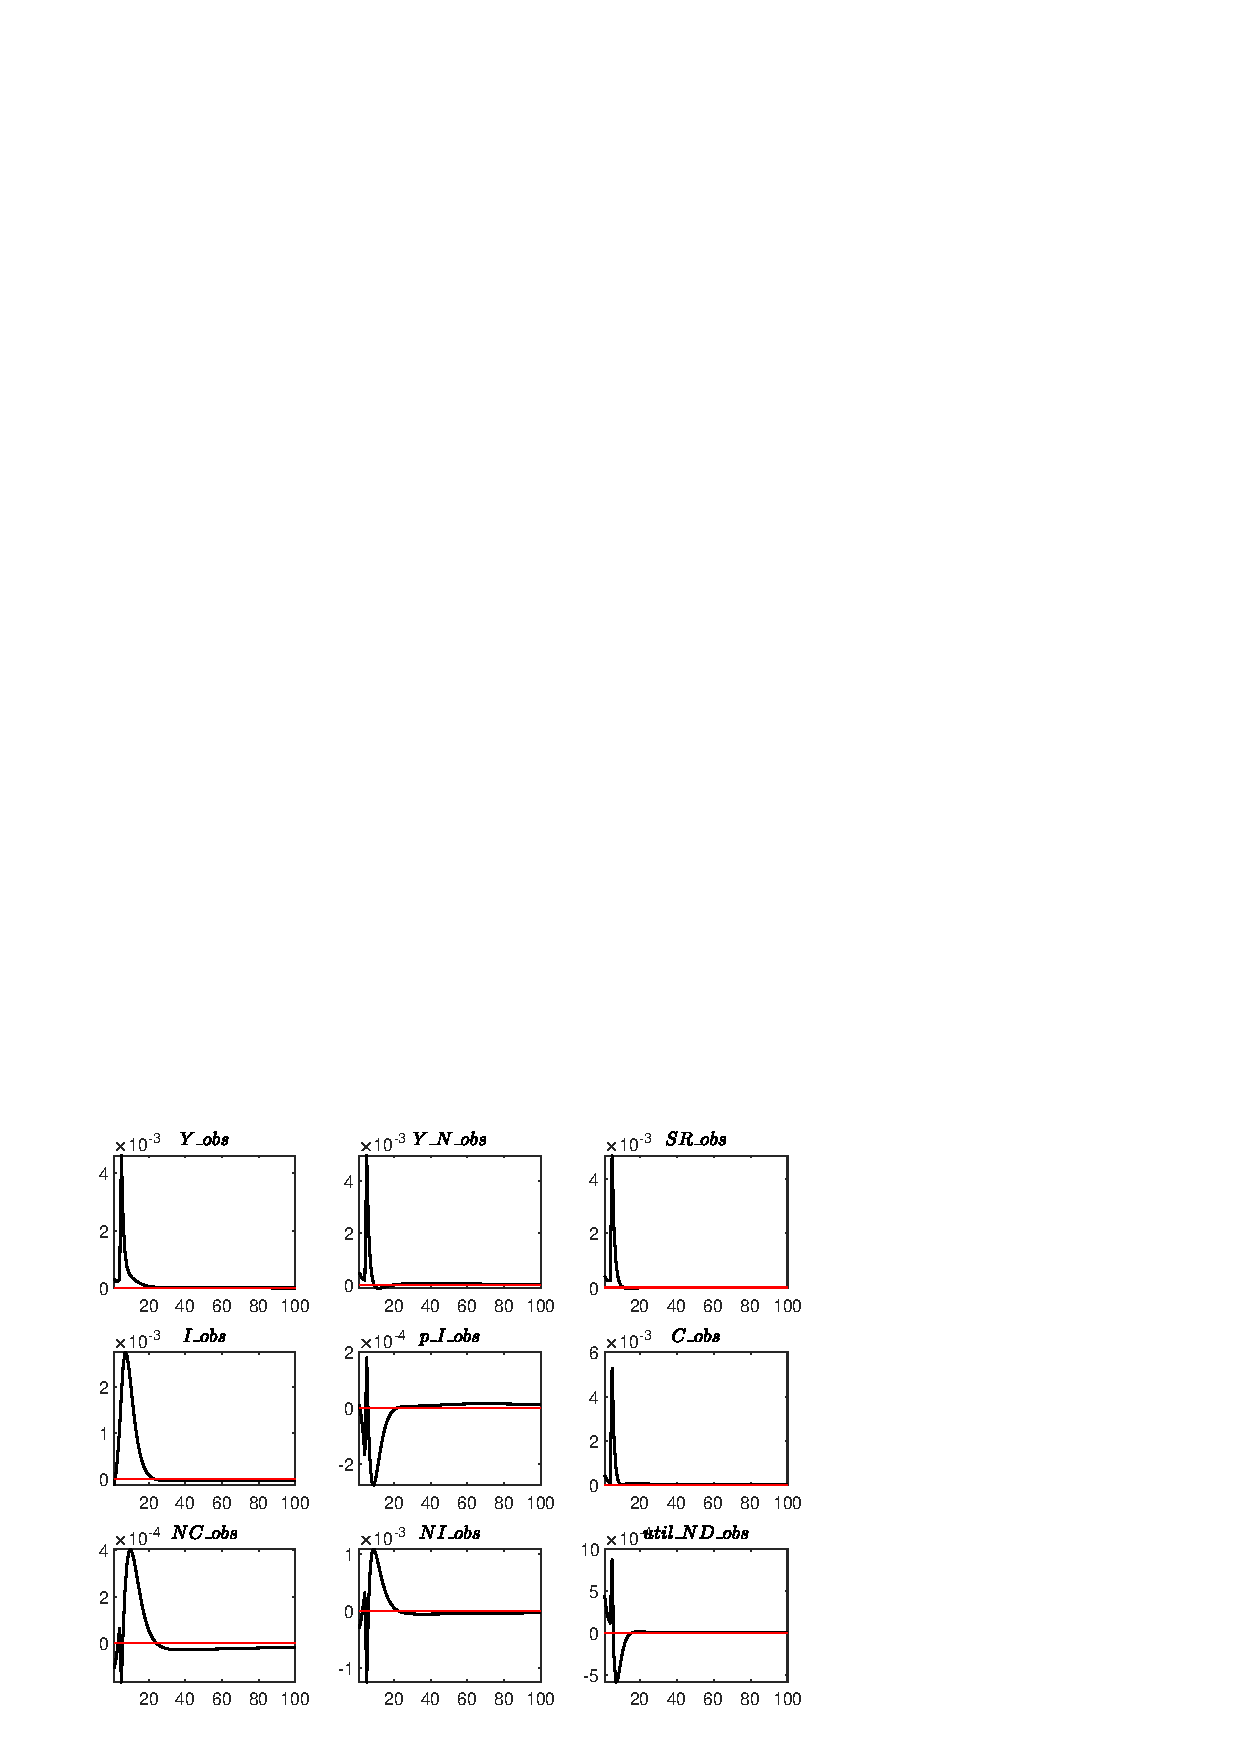
\includegraphics[width=0.80\textwidth]{BRS_sectoral/graphs/BRS_sectoral_IRF_e_g_news1}
\caption{Impulse response functions (orthogonalized shock to ${e_{g,-4}}$).}\label{Fig:IRF:e_g_news:1}
\end{figure}
 
\begin{figure}[H]
\centering 
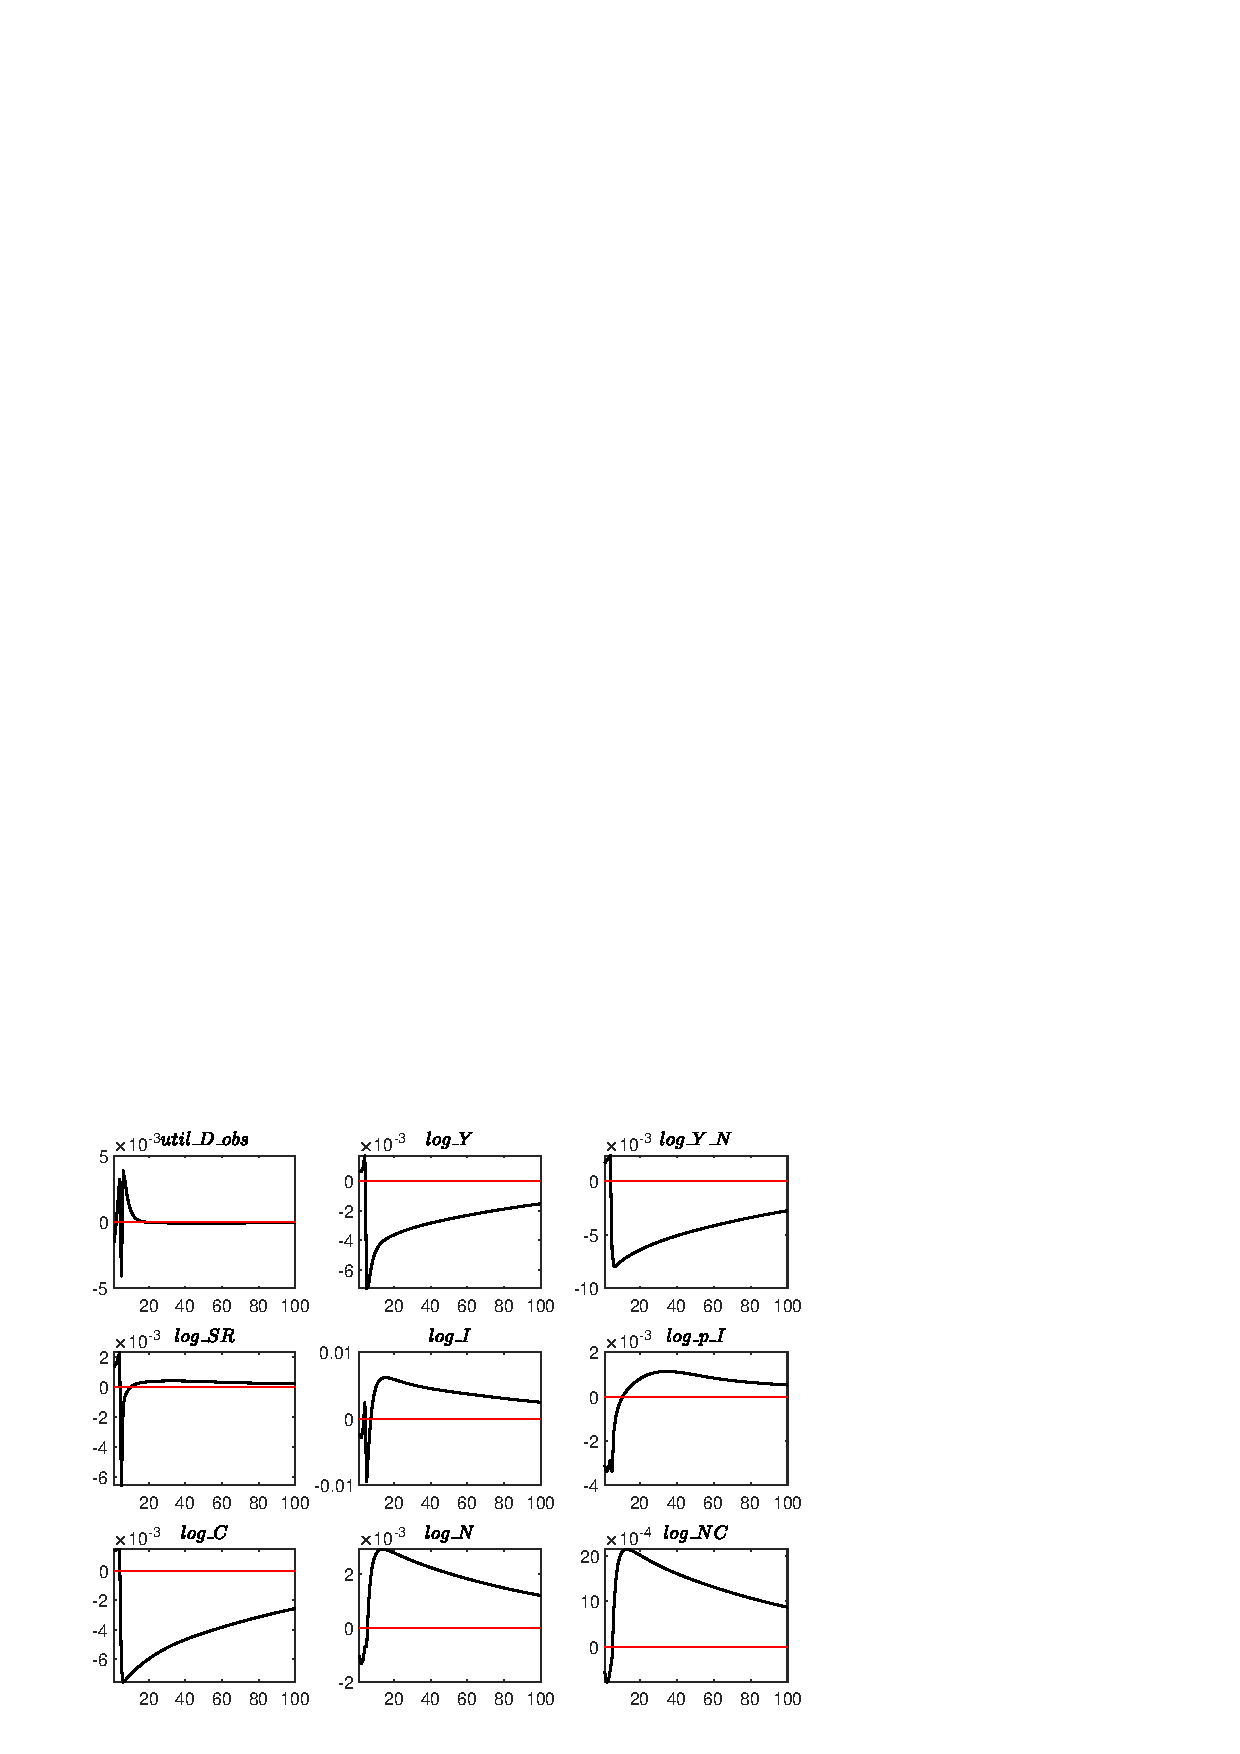
\includegraphics[width=0.80\textwidth]{BRS_sectoral/graphs/BRS_sectoral_IRF_e_g_news2}
\caption{Impulse response functions (orthogonalized shock to ${e_{g,-4}}$).}\label{Fig:IRF:e_g_news:2}
\end{figure}
 
\begin{figure}[H]
\centering 
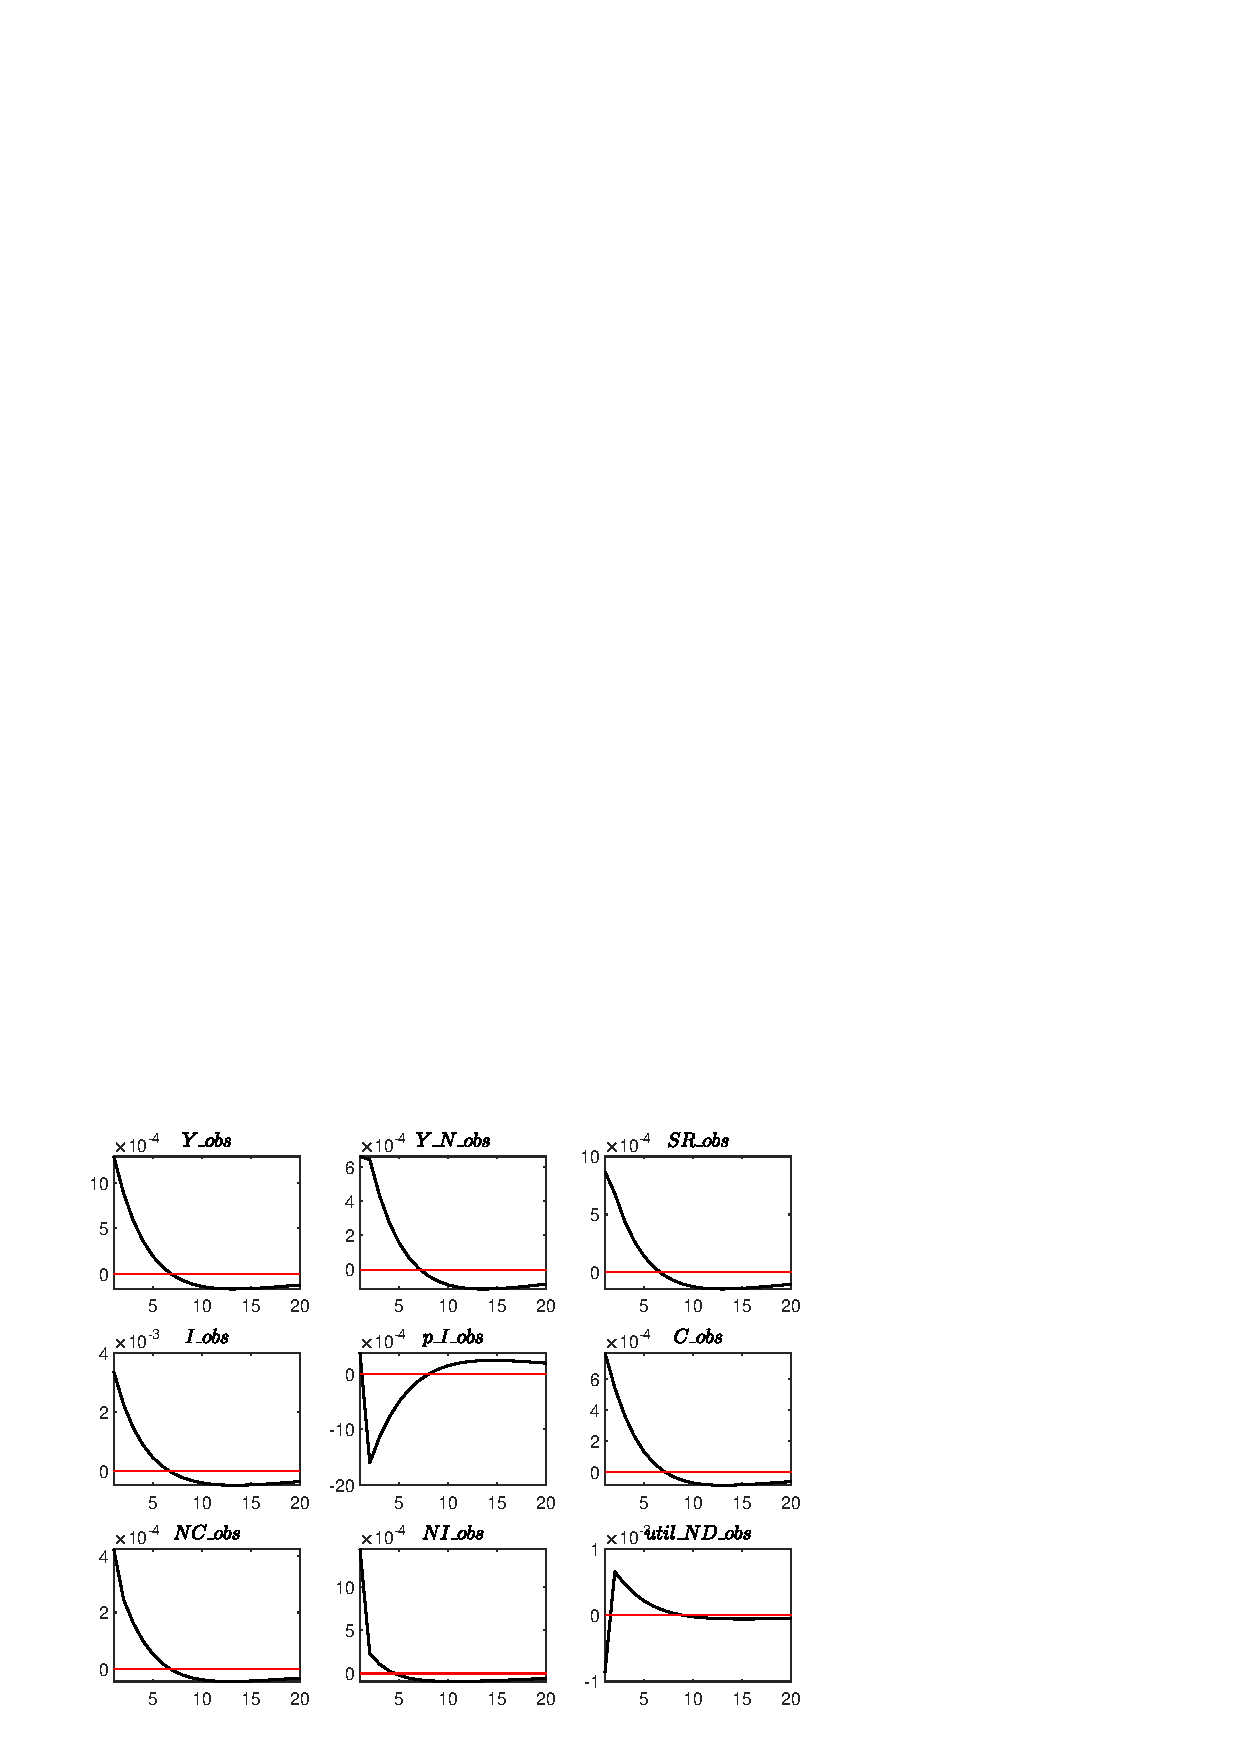
\includegraphics[width=0.80\textwidth]{BRS_sectoral/graphs/BRS_sectoral_IRF_e_Z1}
\caption{Impulse response functions (orthogonalized shock to ${e_Z}$).}\label{Fig:IRF:e_Z:1}
\end{figure}
 
\begin{figure}[H]
\centering 
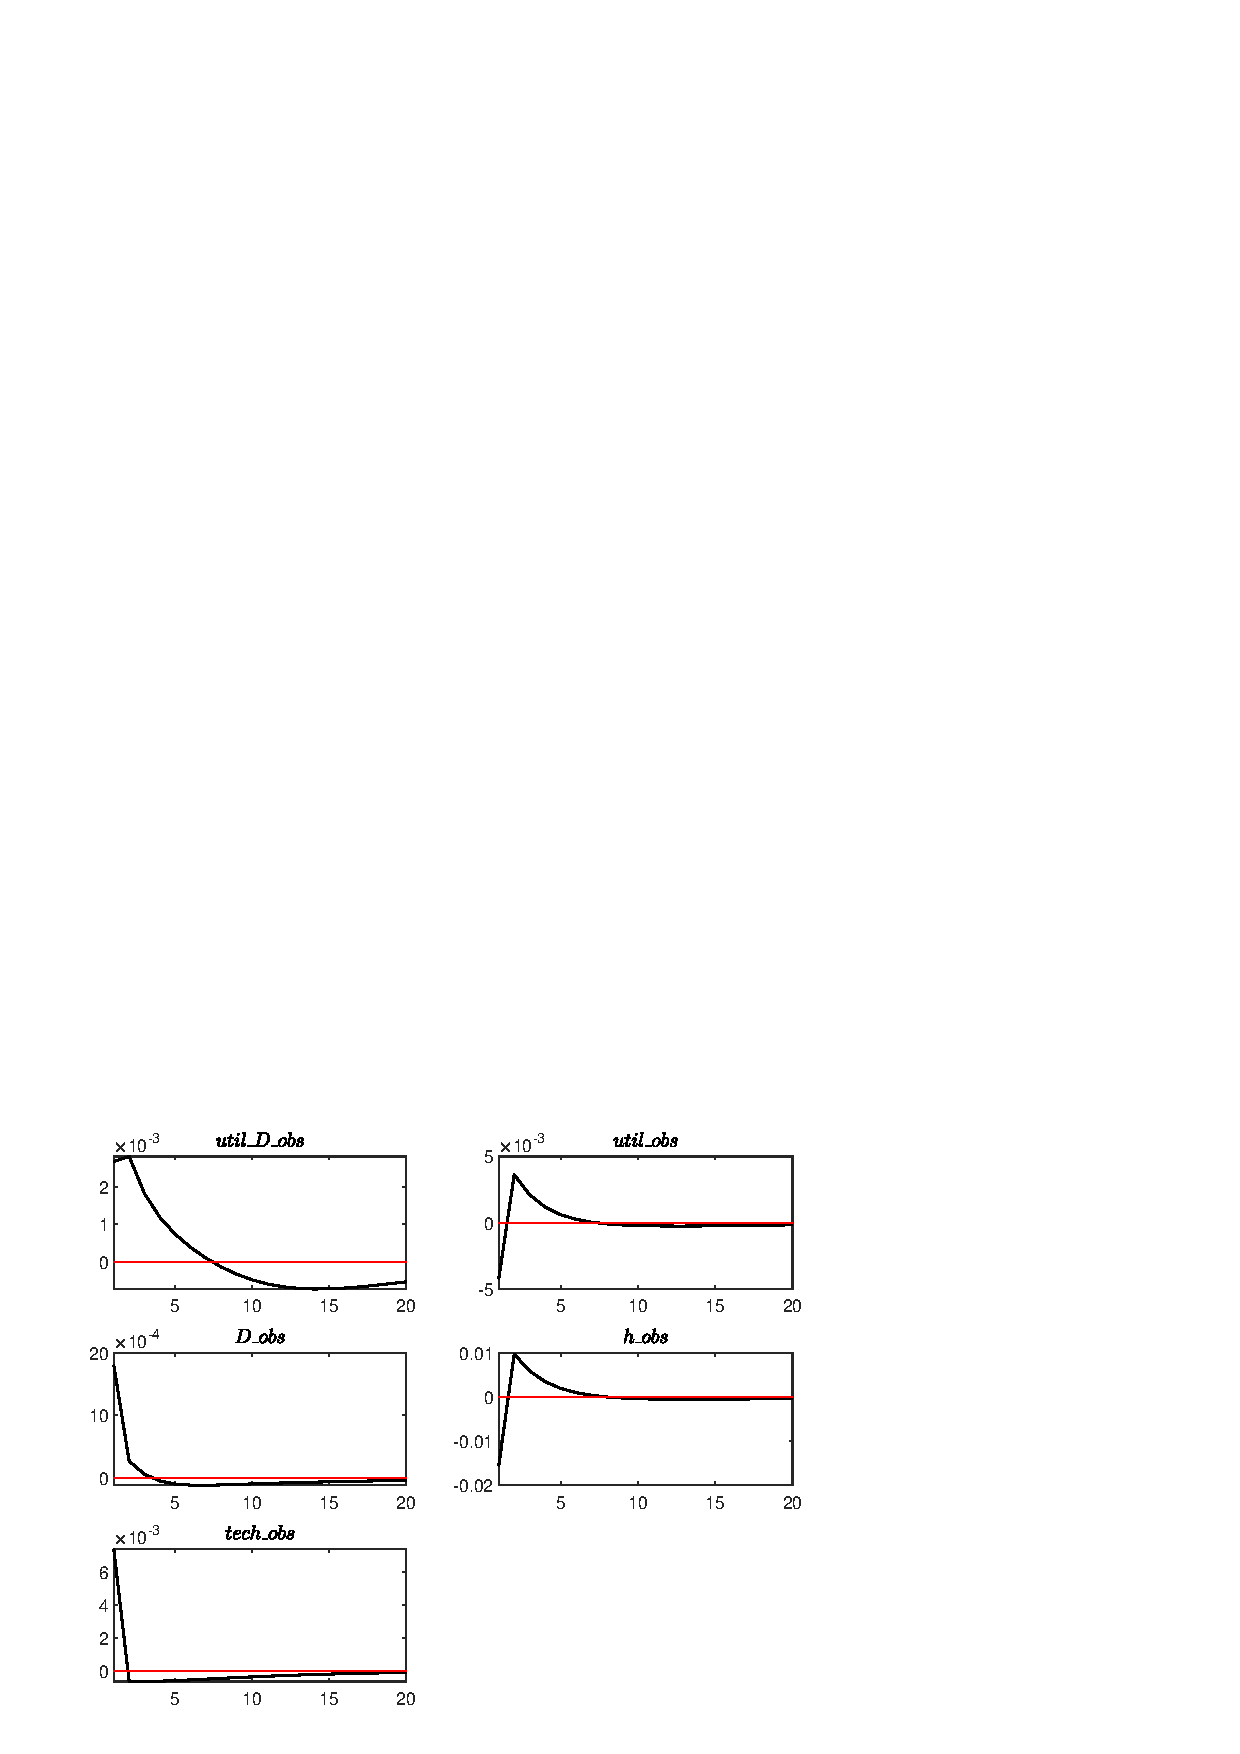
\includegraphics[width=0.80\textwidth]{BRS_sectoral/graphs/BRS_sectoral_IRF_e_Z2}
\caption{Impulse response functions (orthogonalized shock to ${e_Z}$).}\label{Fig:IRF:e_Z:2}
\end{figure}
 
\begin{figure}[H]
\centering 
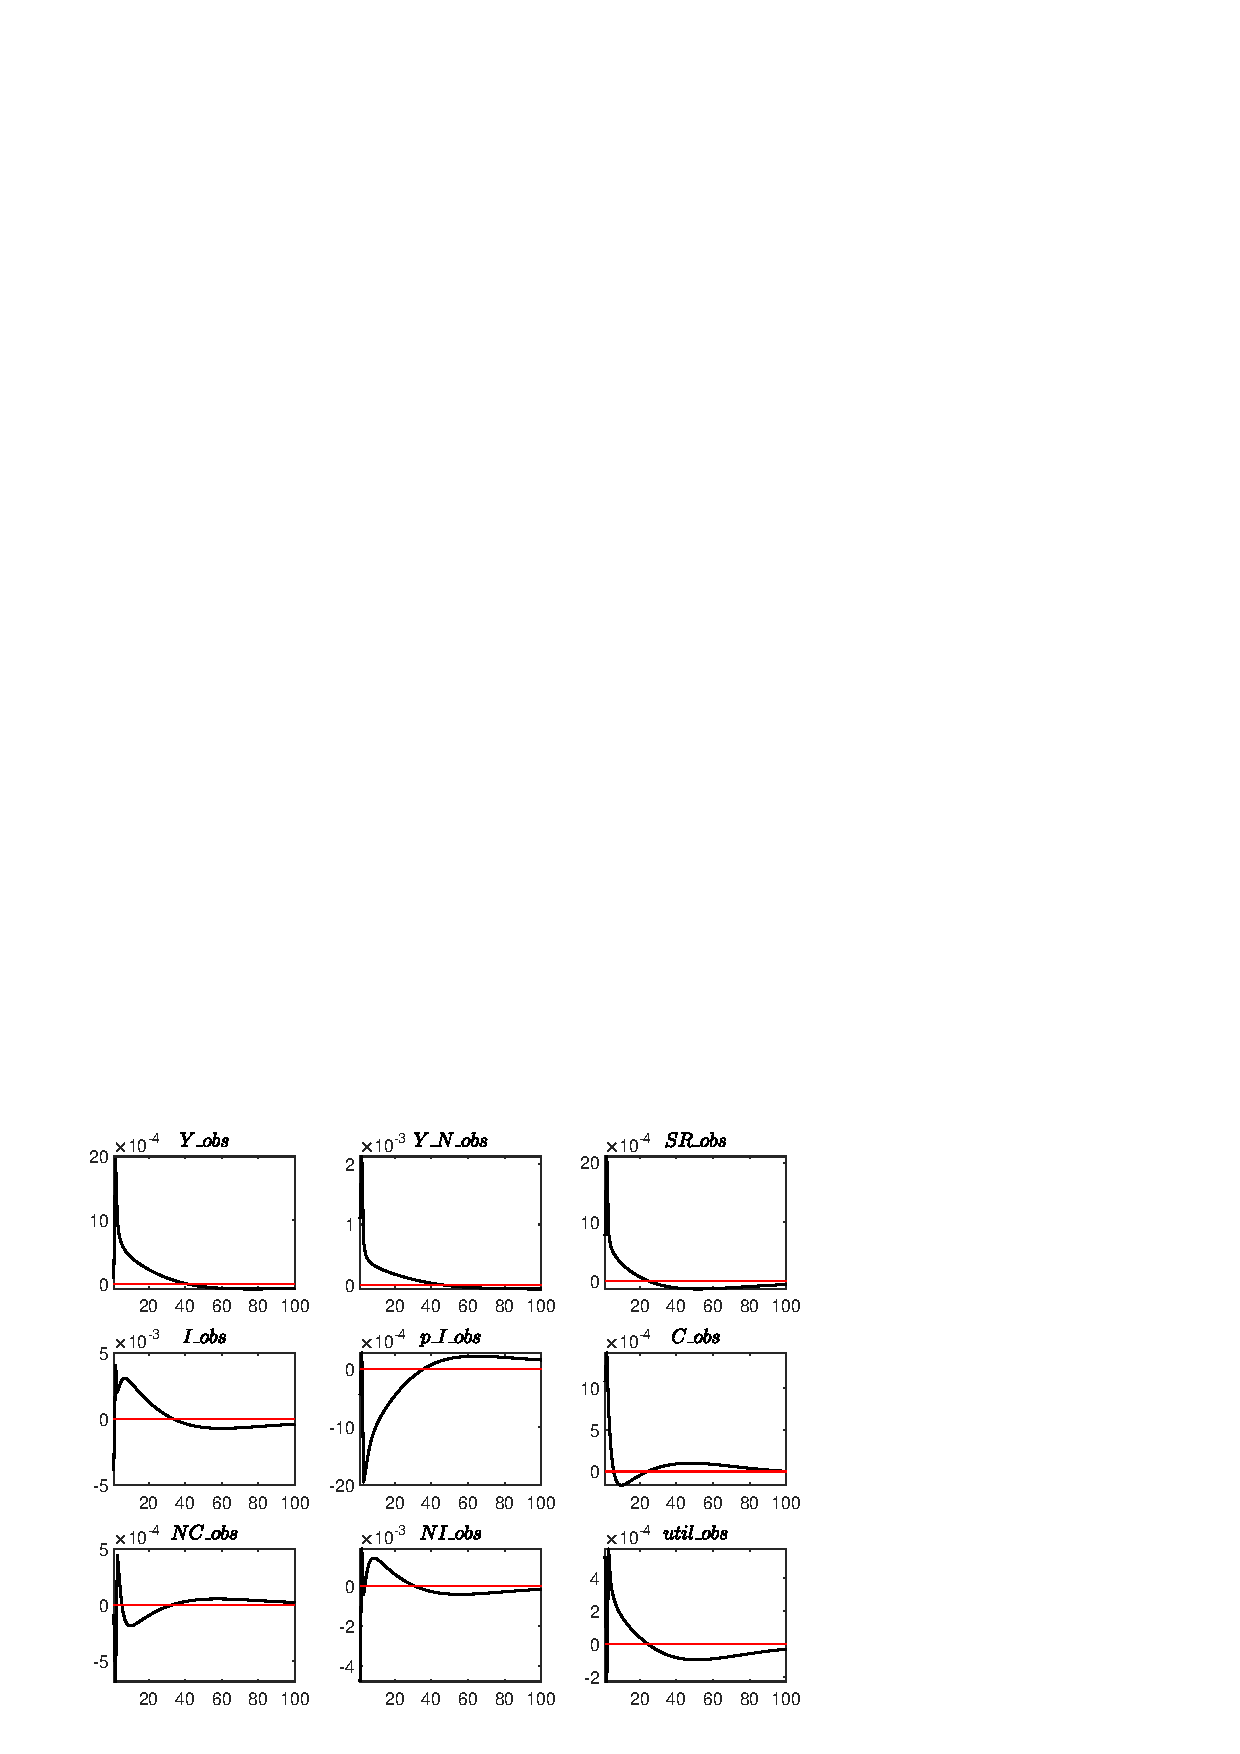
\includegraphics[width=0.80\textwidth]{BRS_sectoral/graphs/BRS_sectoral_IRF_e_Z_news1}
\caption{Impulse response functions (orthogonalized shock to ${e_{Z,-4}}$).}\label{Fig:IRF:e_Z_news:1}
\end{figure}
 
\begin{figure}[H]
\centering 
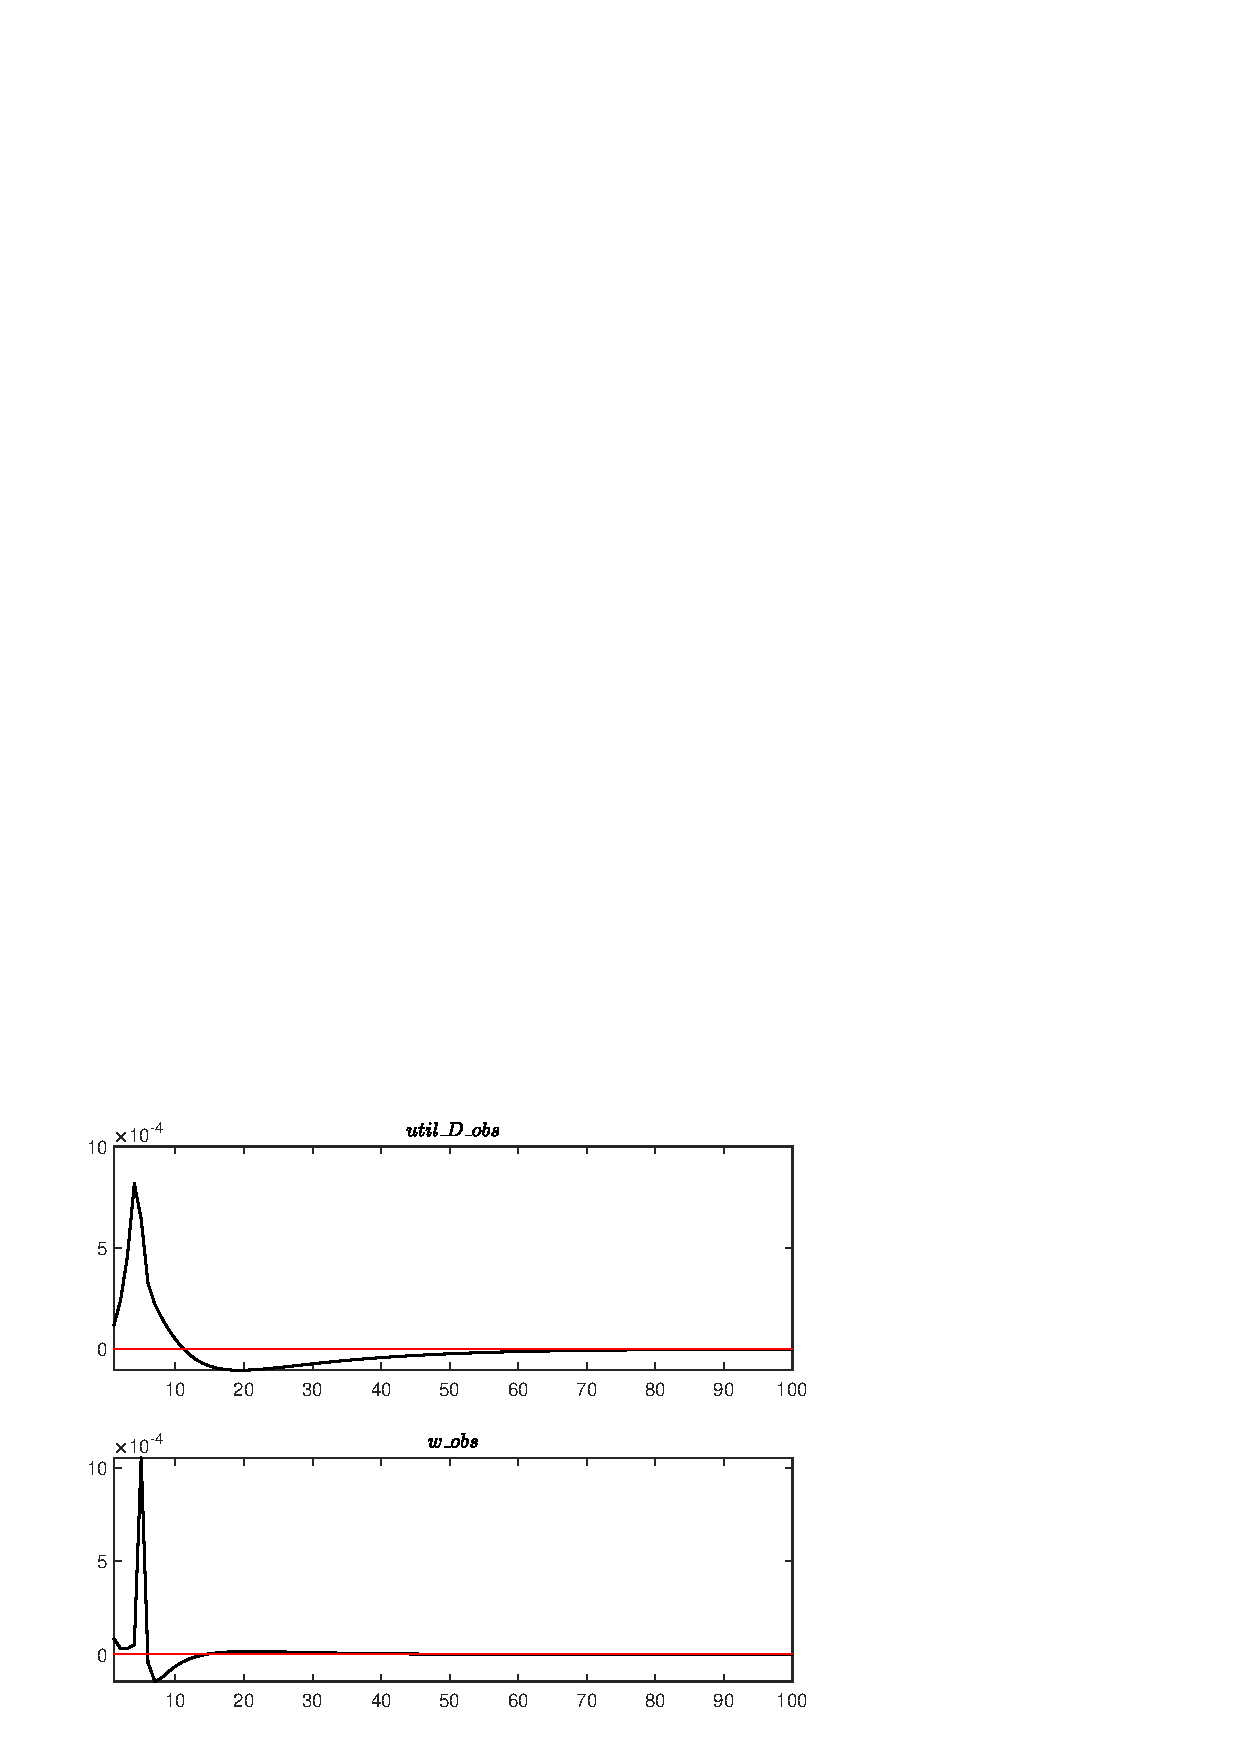
\includegraphics[width=0.80\textwidth]{BRS_sectoral/graphs/BRS_sectoral_IRF_e_Z_news2}
\caption{Impulse response functions (orthogonalized shock to ${e_{Z,-4}}$).}\label{Fig:IRF:e_Z_news:2}
\end{figure}
 
\begin{figure}[H]
\centering 
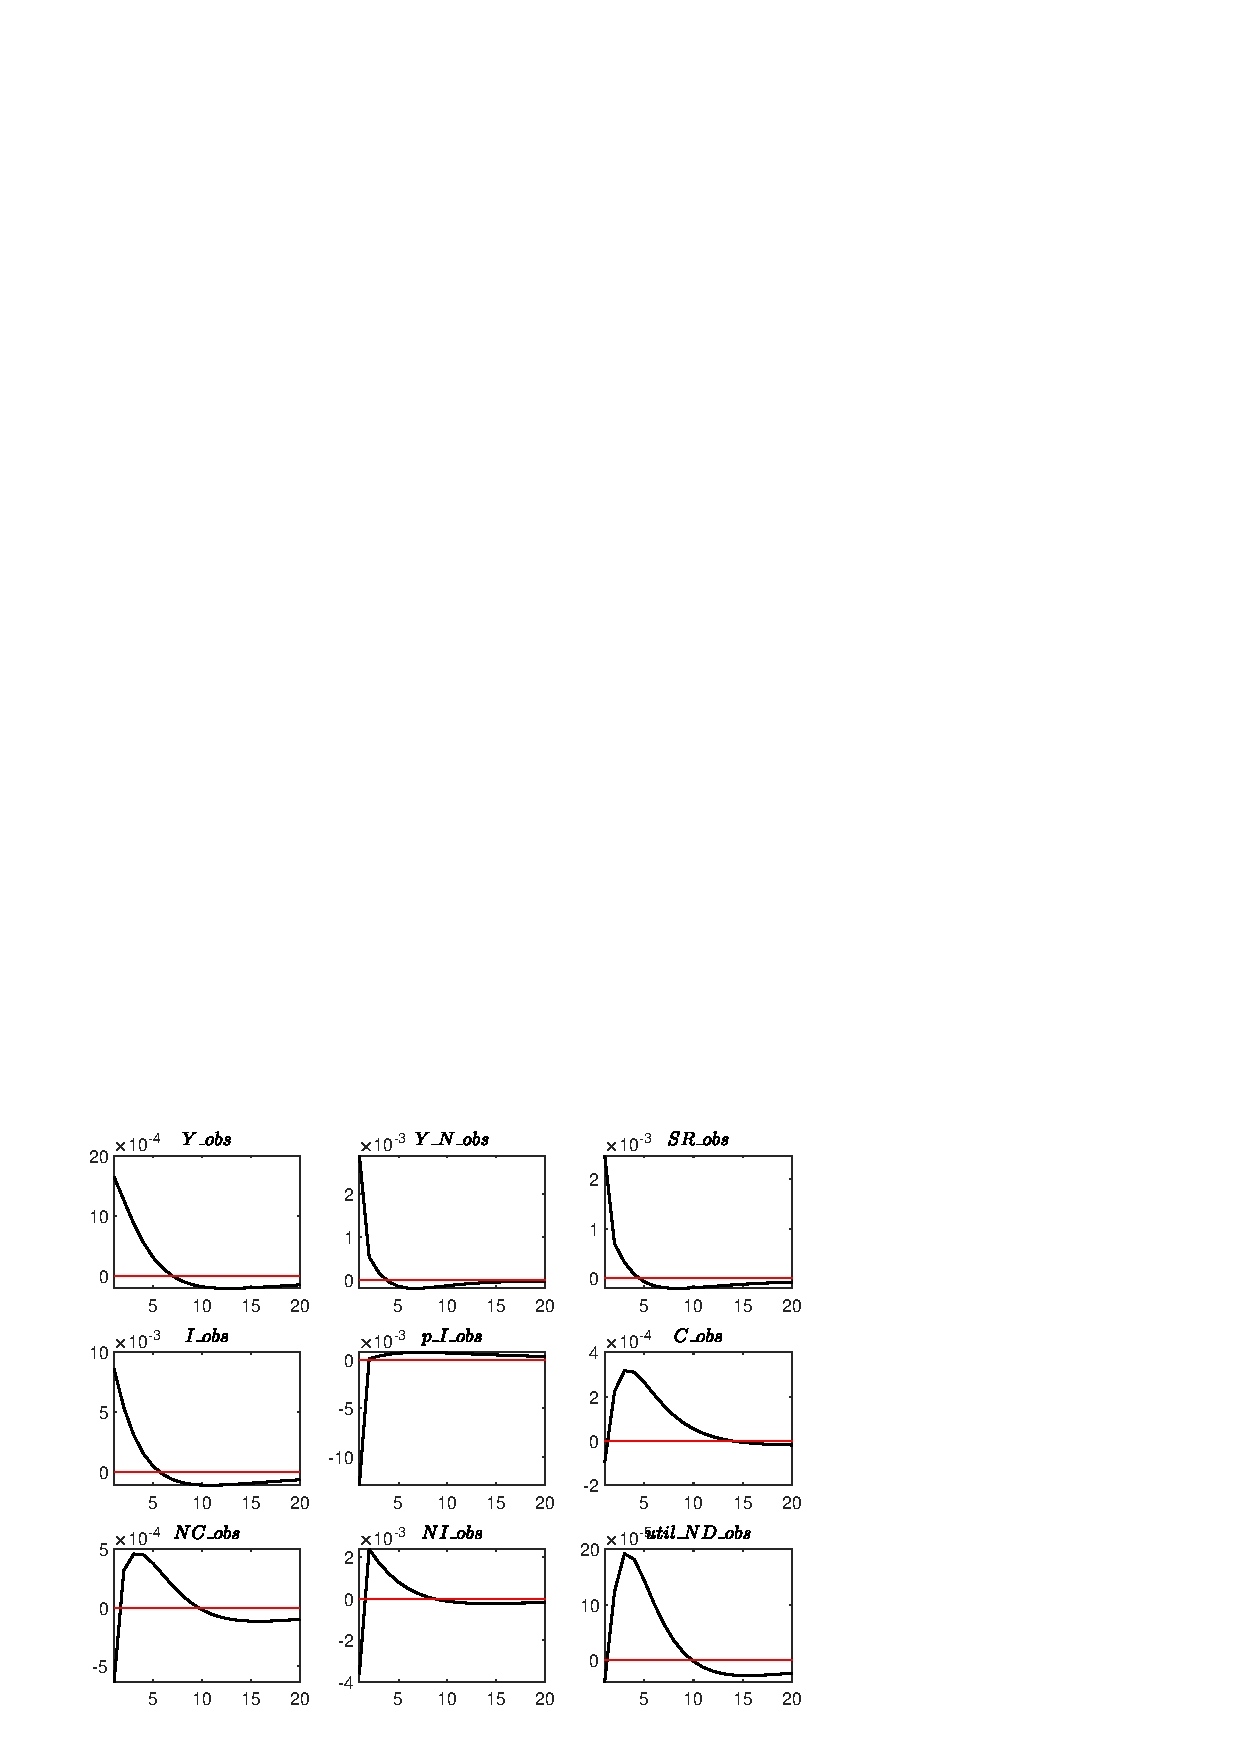
\includegraphics[width=0.80\textwidth]{BRS_sectoral/graphs/BRS_sectoral_IRF_e_ZI1}
\caption{Impulse response functions (orthogonalized shock to ${e_{ZI}}$).}\label{Fig:IRF:e_ZI:1}
\end{figure}
 
\begin{figure}[H]
\centering 
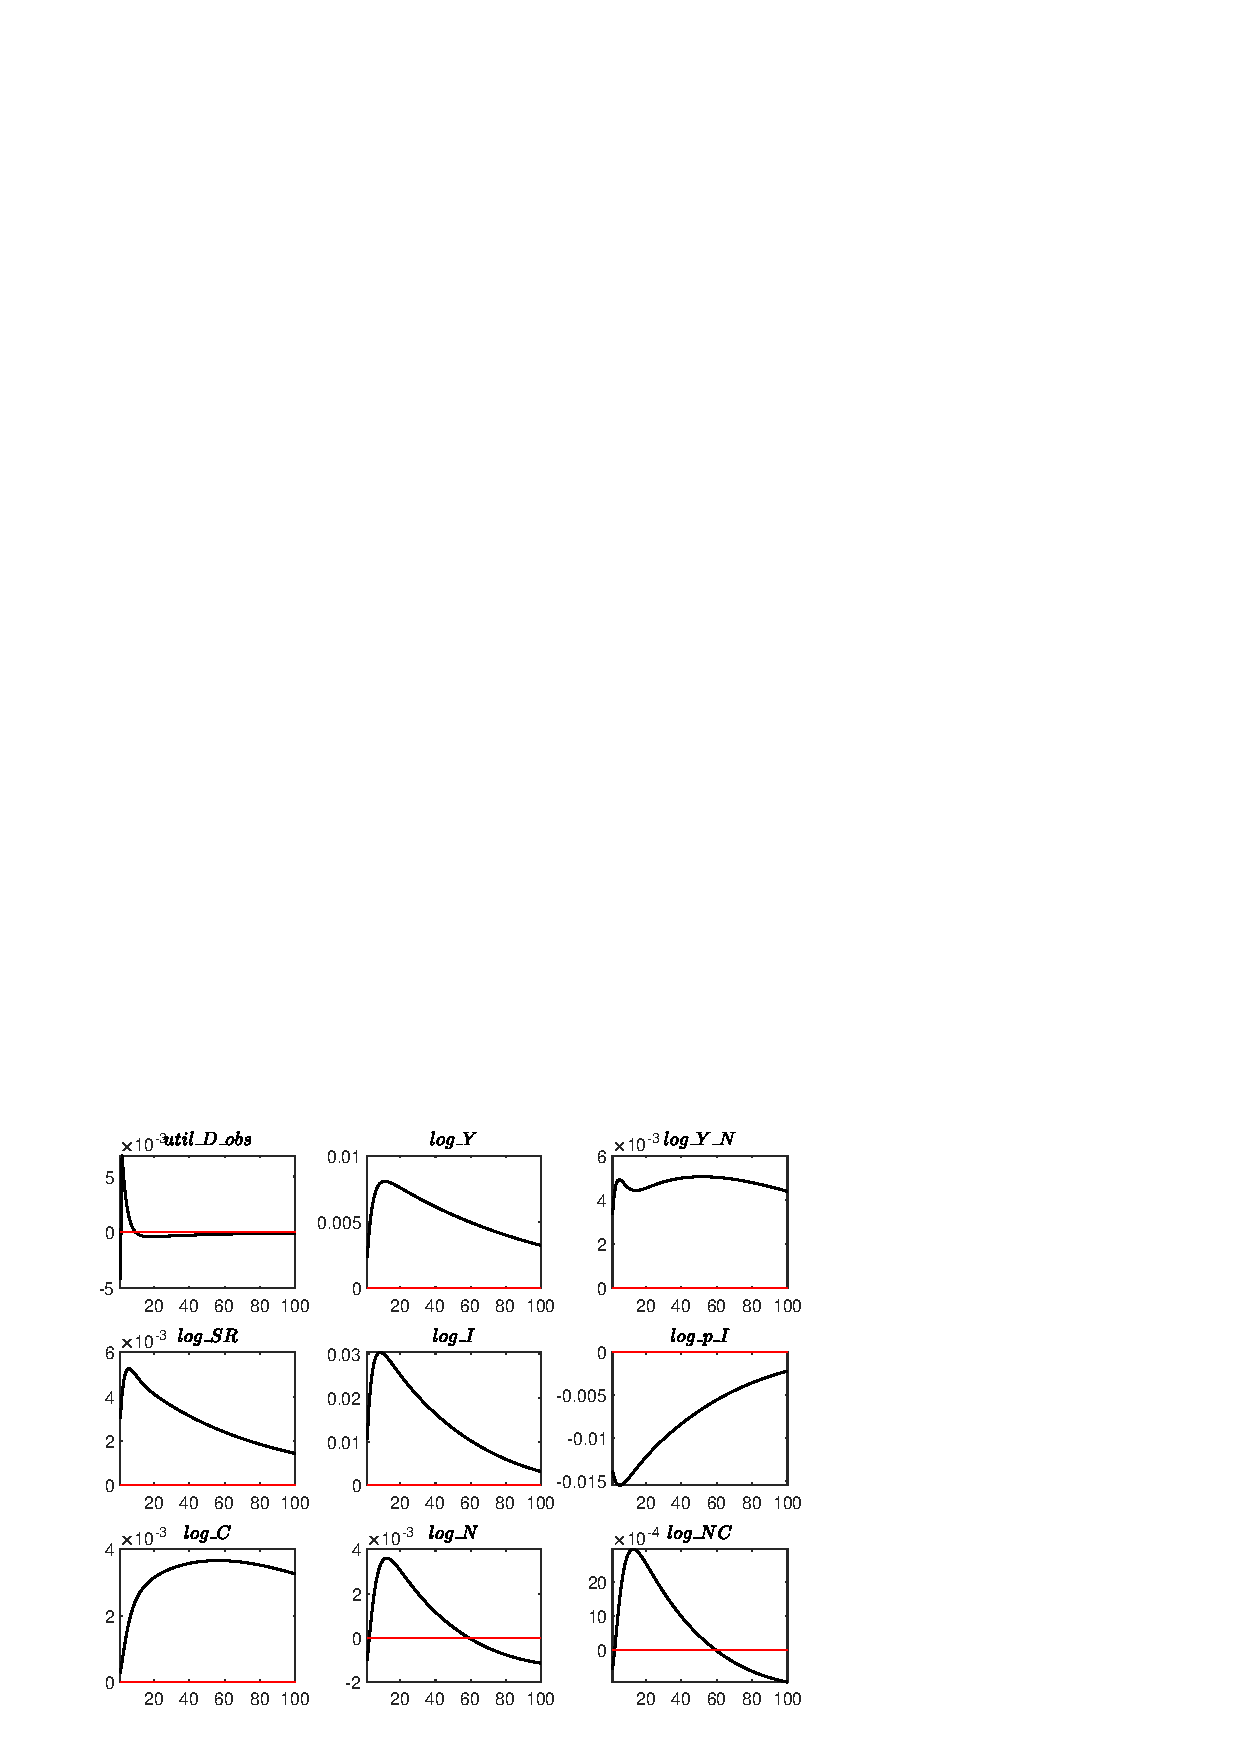
\includegraphics[width=0.80\textwidth]{BRS_sectoral/graphs/BRS_sectoral_IRF_e_ZI2}
\caption{Impulse response functions (orthogonalized shock to ${e_{ZI}}$).}\label{Fig:IRF:e_ZI:2}
\end{figure}
 
\begin{figure}[H]
\centering 
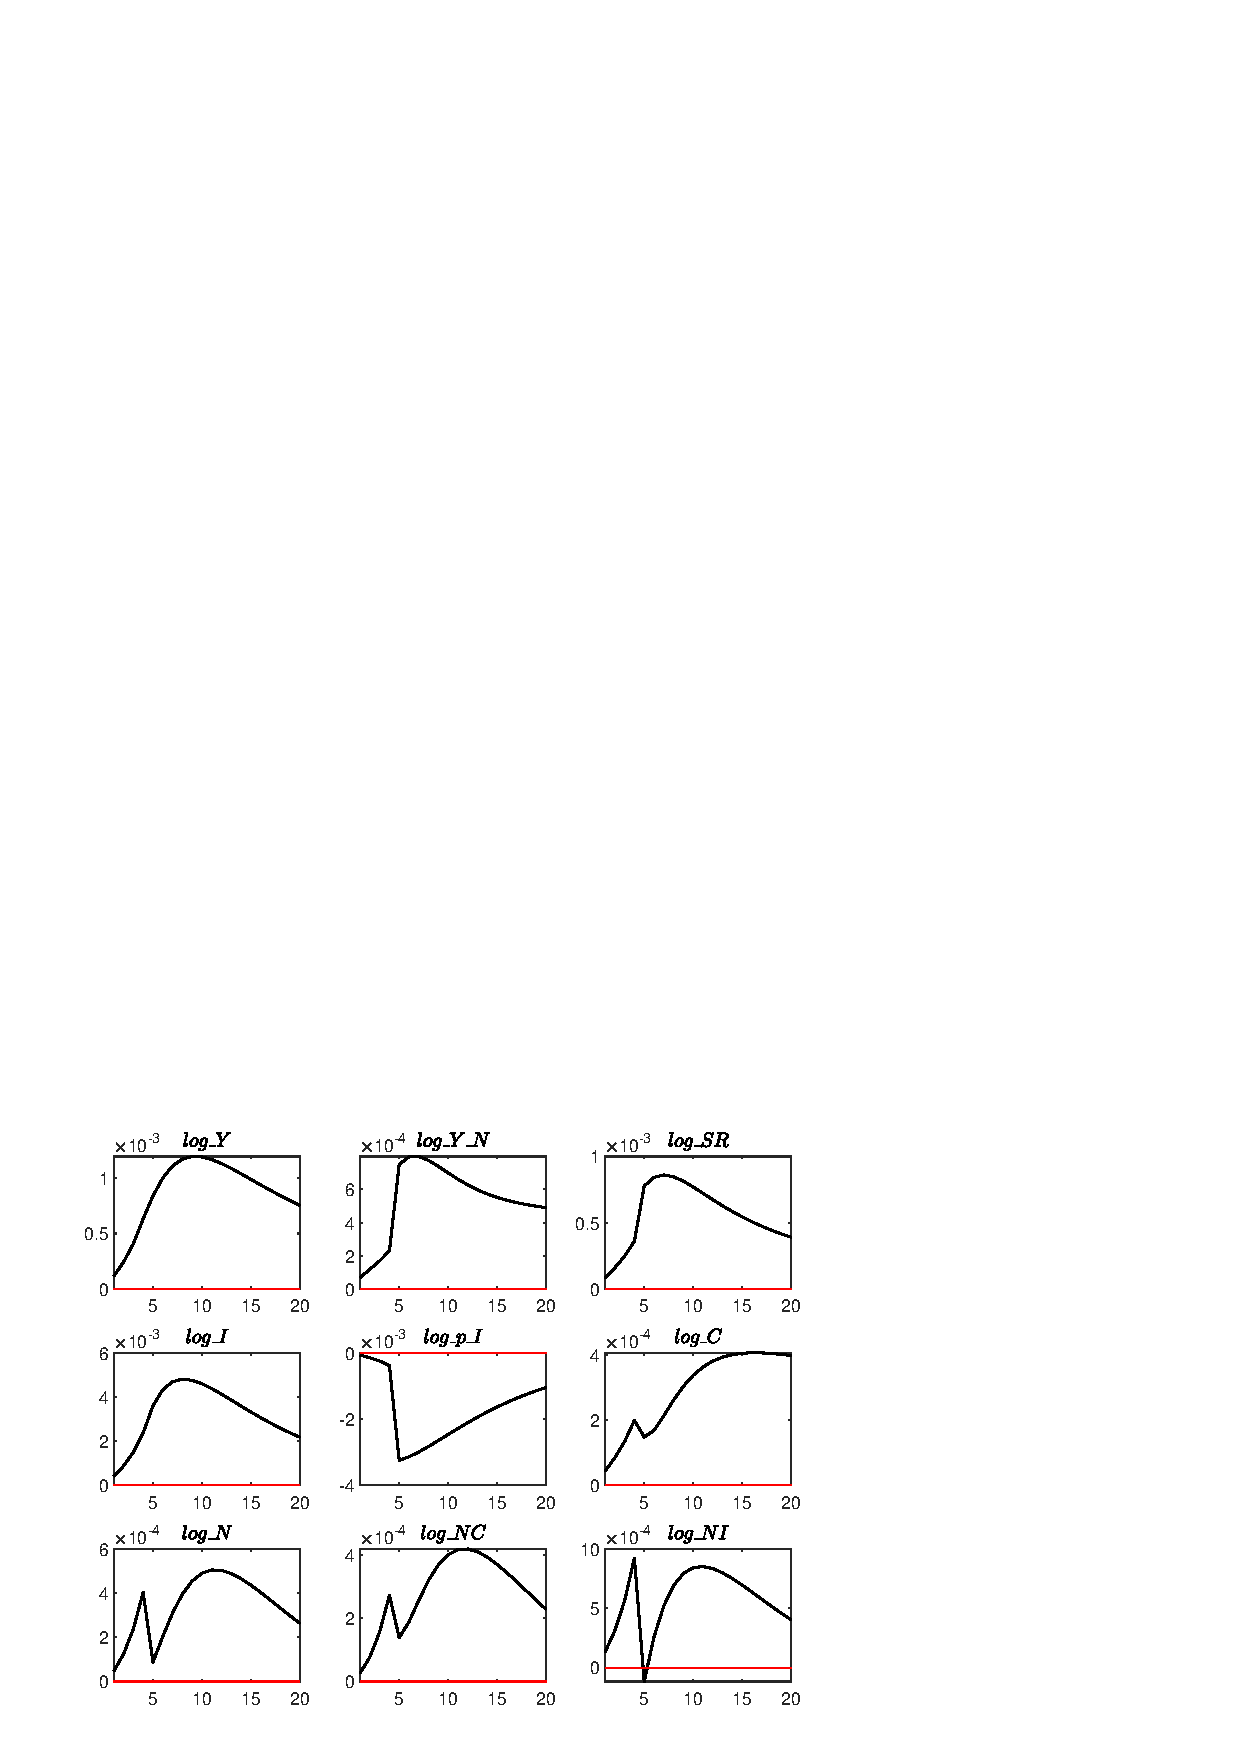
\includegraphics[width=0.80\textwidth]{BRS_sectoral/graphs/BRS_sectoral_IRF_e_ZI_news1}
\caption{Impulse response functions (orthogonalized shock to ${e_{ZI,-4}}$).}\label{Fig:IRF:e_ZI_news:1}
\end{figure}
 
\begin{figure}[H]
\centering 
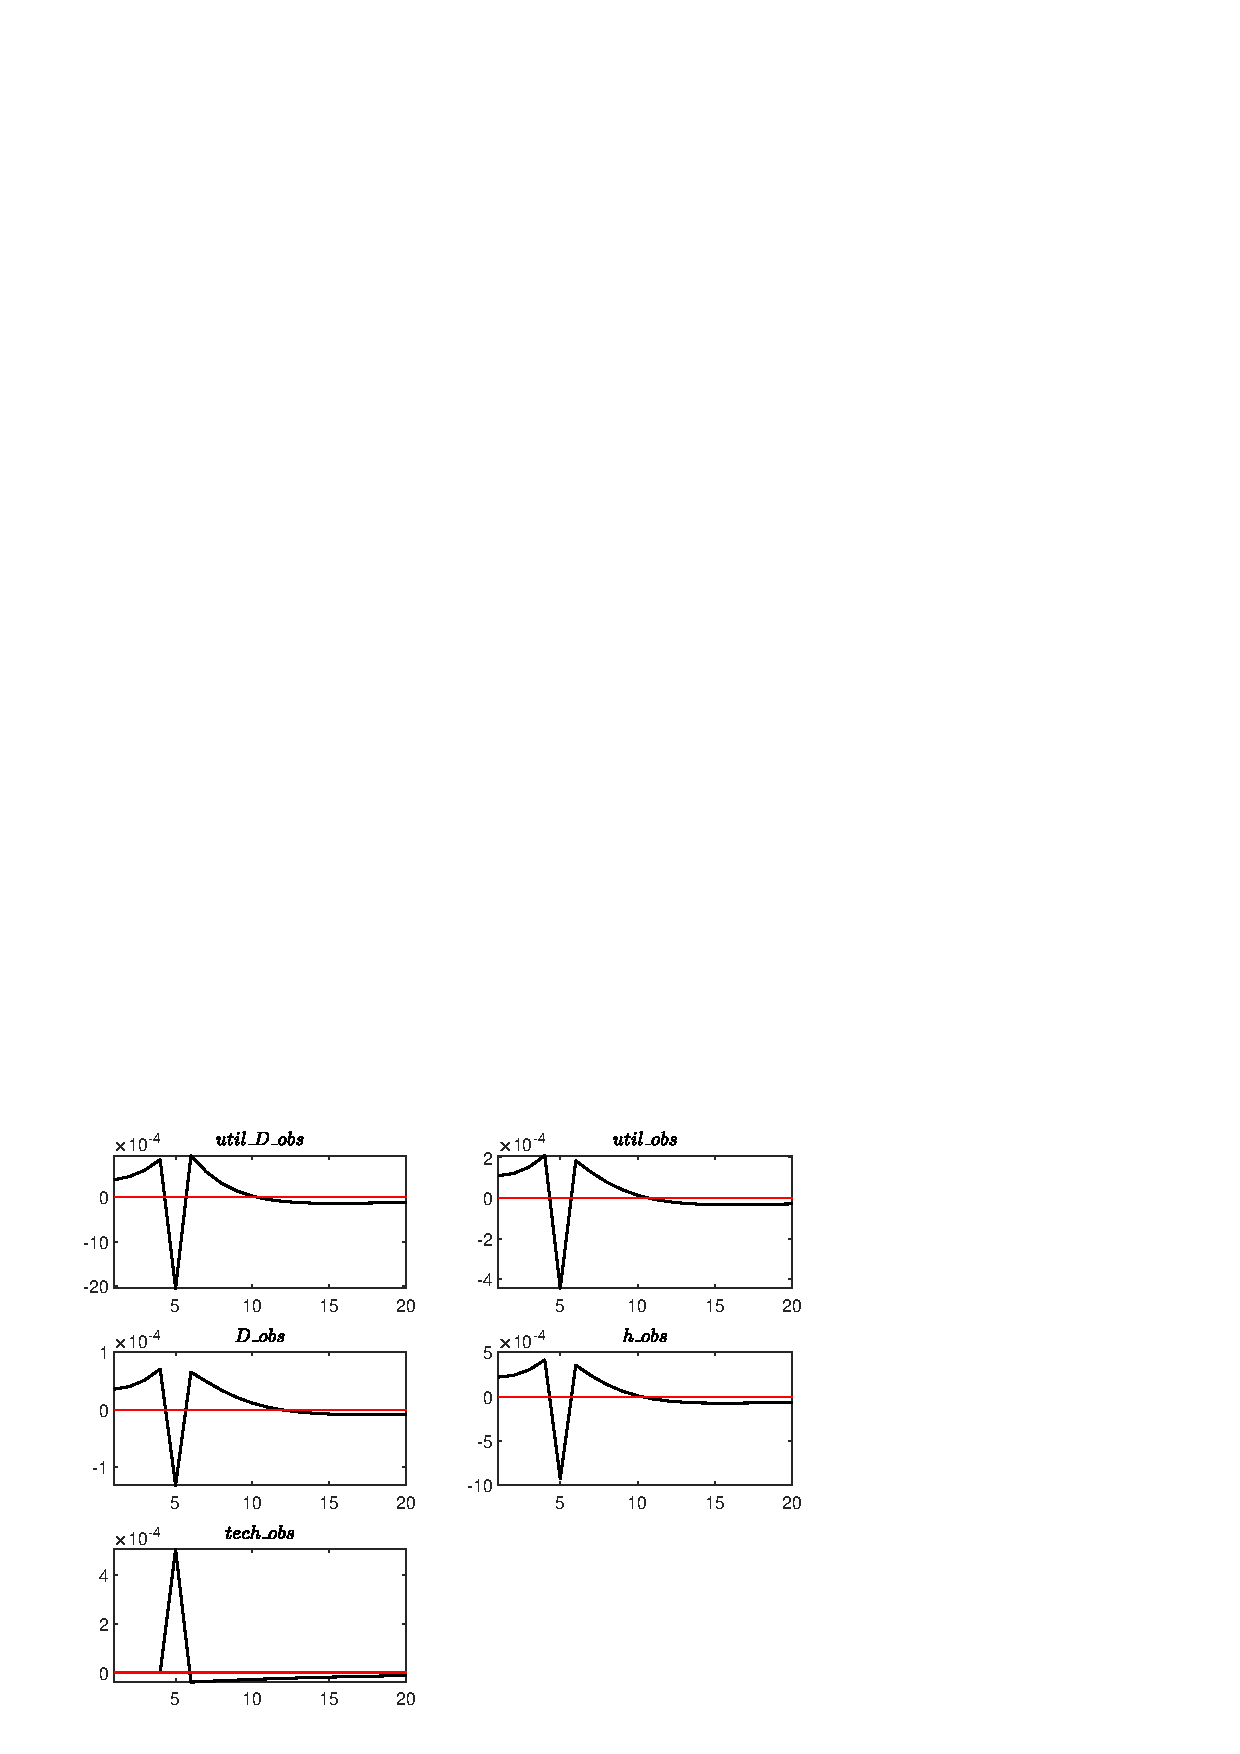
\includegraphics[width=0.80\textwidth]{BRS_sectoral/graphs/BRS_sectoral_IRF_e_ZI_news2}
\caption{Impulse response functions (orthogonalized shock to ${e_{ZI,-4}}$).}\label{Fig:IRF:e_ZI_news:2}
\end{figure}
 
\begin{figure}[H]
\centering 
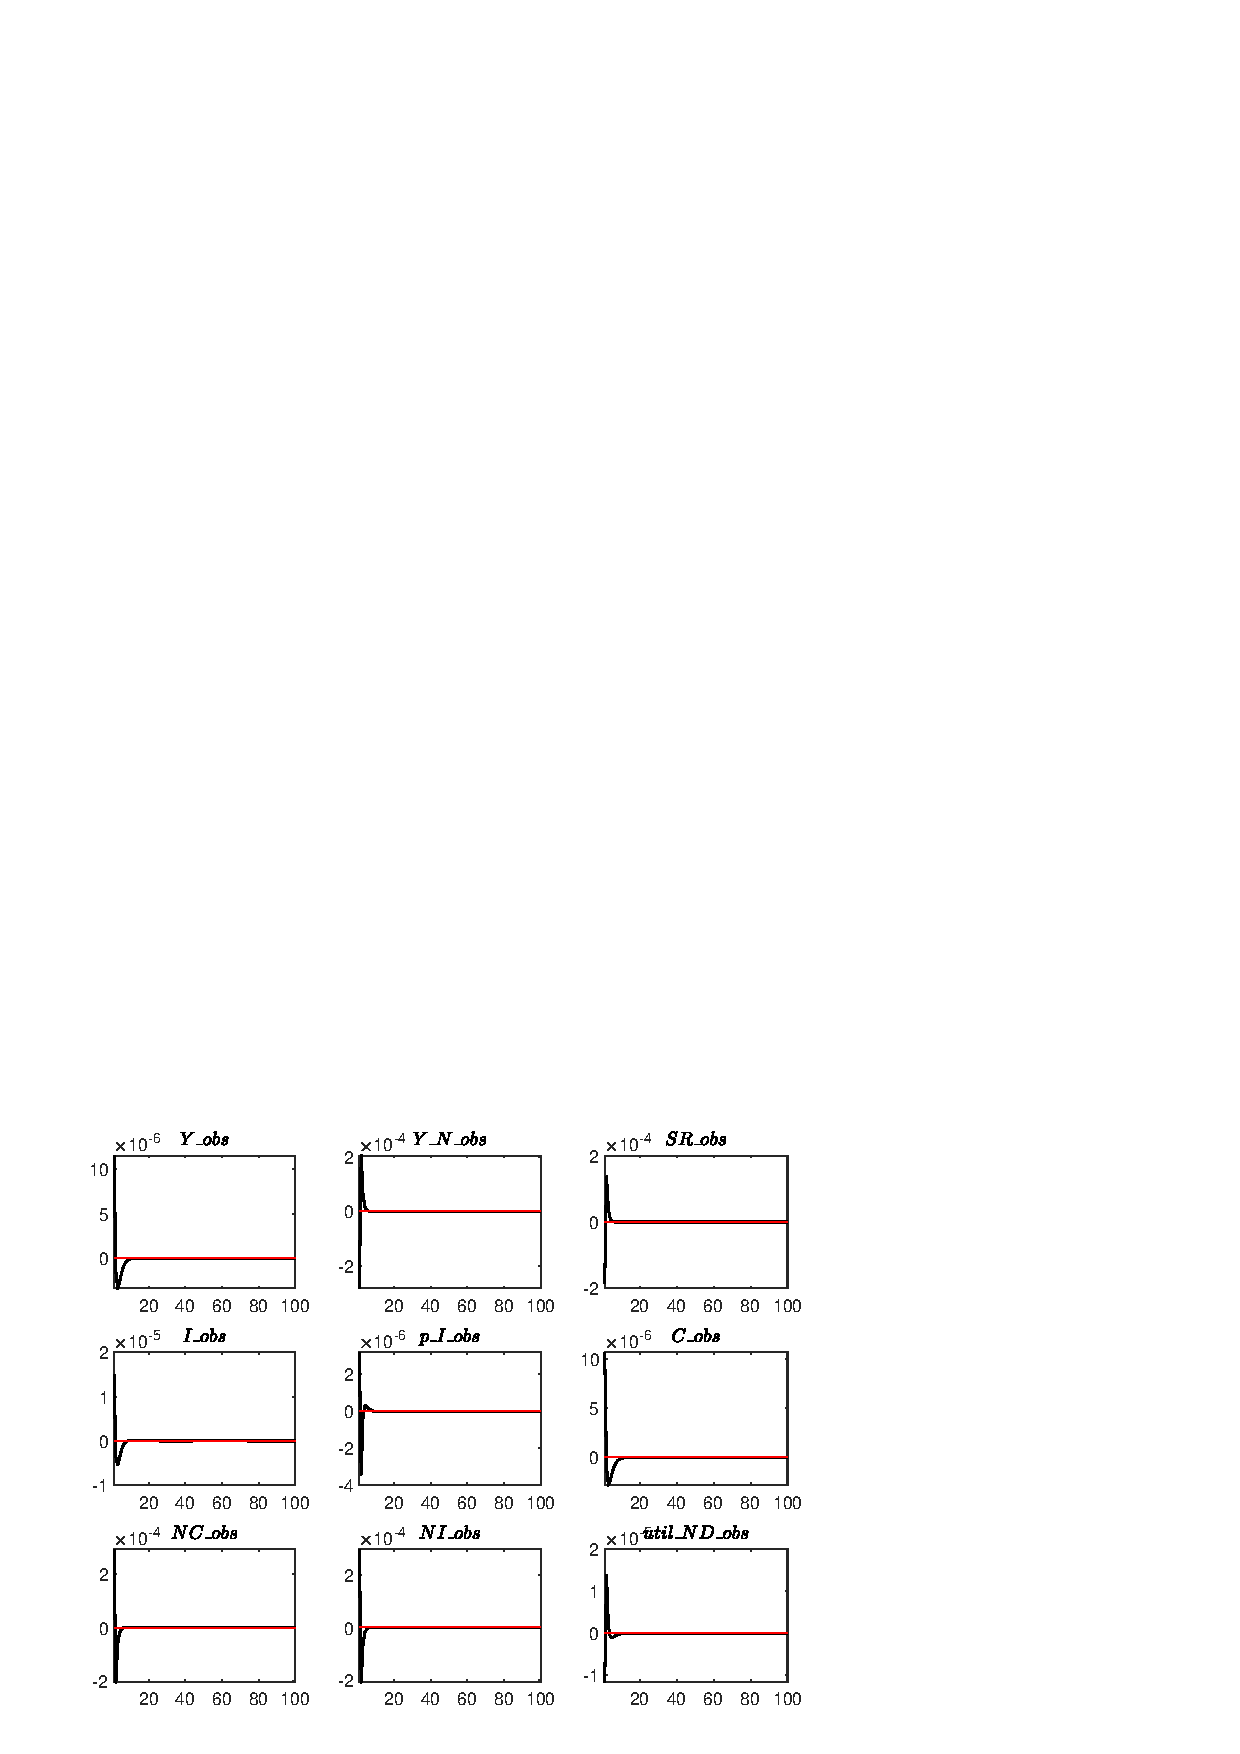
\includegraphics[width=0.80\textwidth]{BRS_sectoral/graphs/BRS_sectoral_IRF_e_N1}
\caption{Impulse response functions (orthogonalized shock to ${e_N}$).}\label{Fig:IRF:e_N:1}
\end{figure}
 
\begin{figure}[H]
\centering 
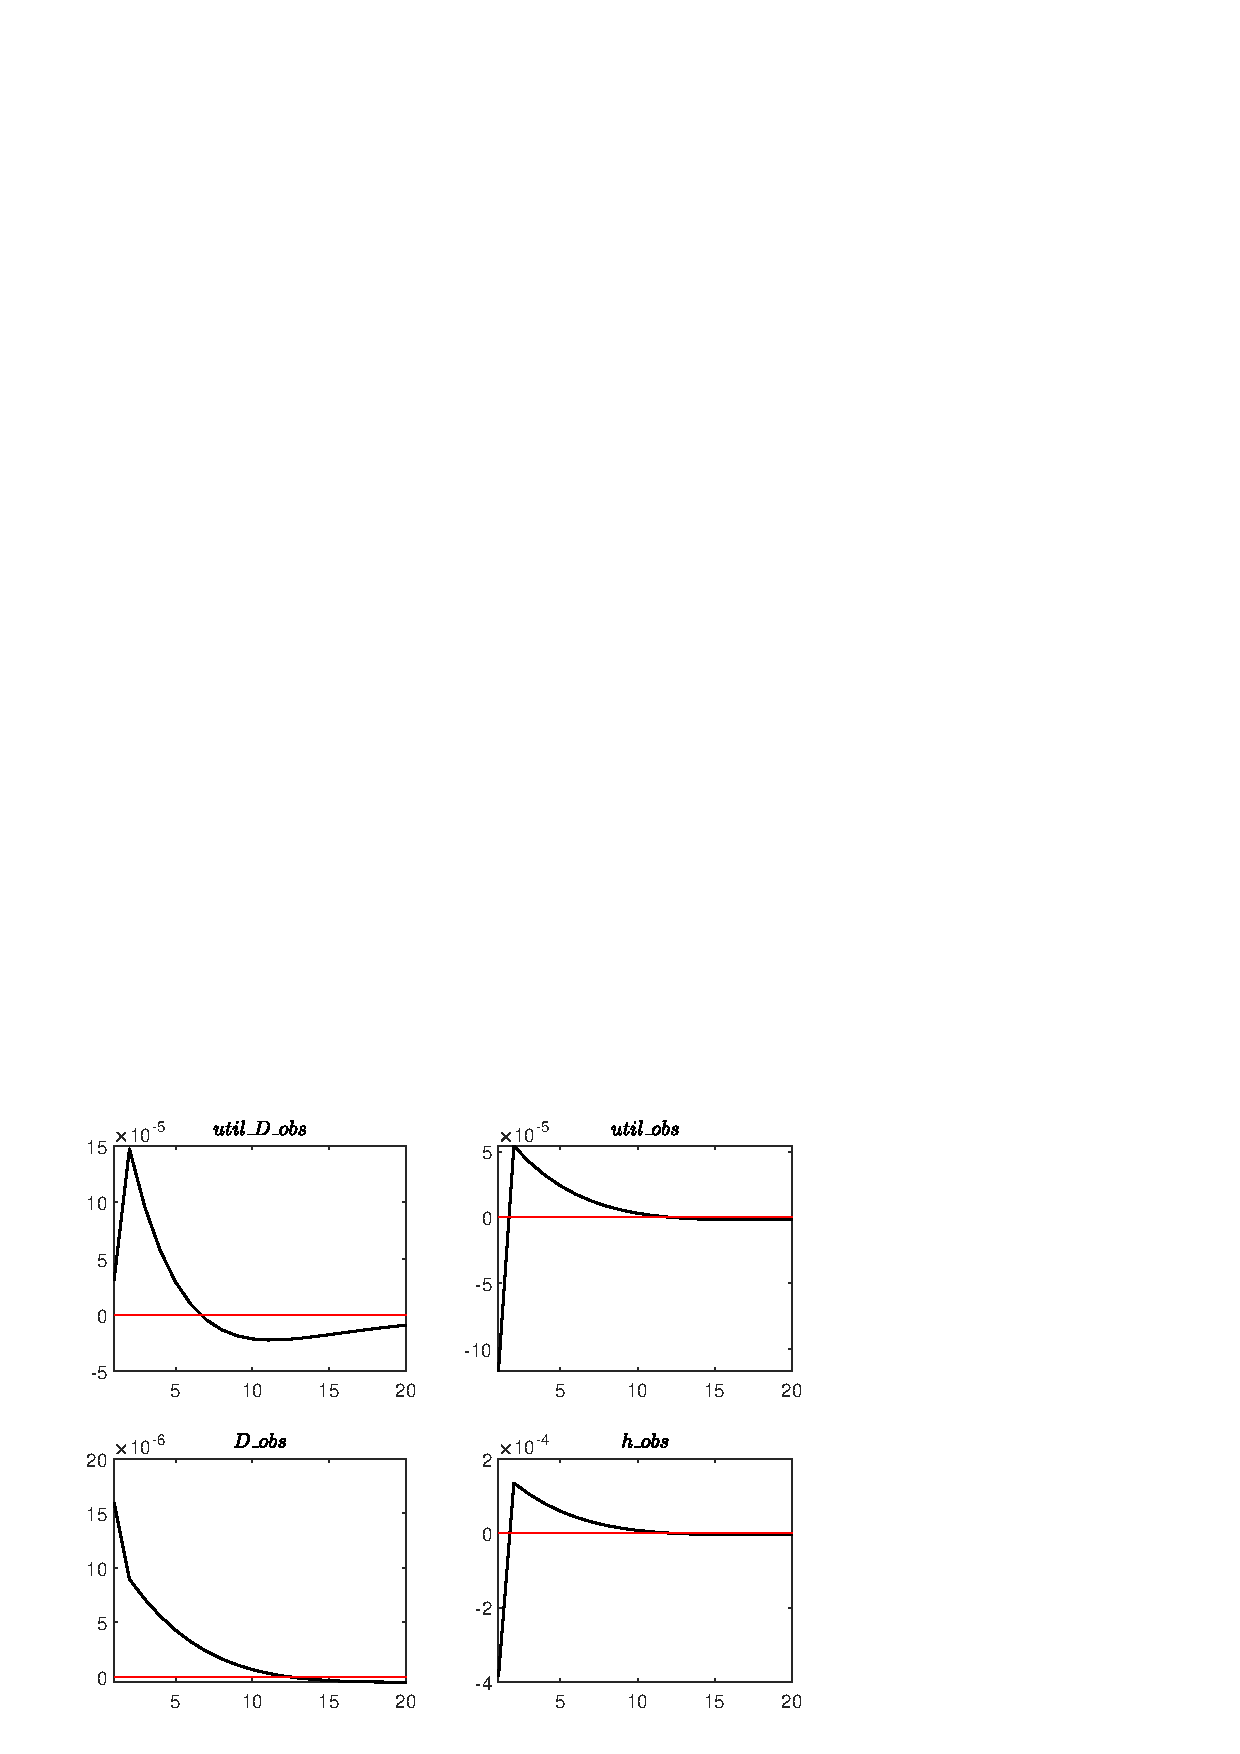
\includegraphics[width=0.80\textwidth]{BRS_sectoral/graphs/BRS_sectoral_IRF_e_N2}
\caption{Impulse response functions (orthogonalized shock to ${e_N}$).}\label{Fig:IRF:e_N:2}
\end{figure}
 
\begin{figure}[H]
\centering 
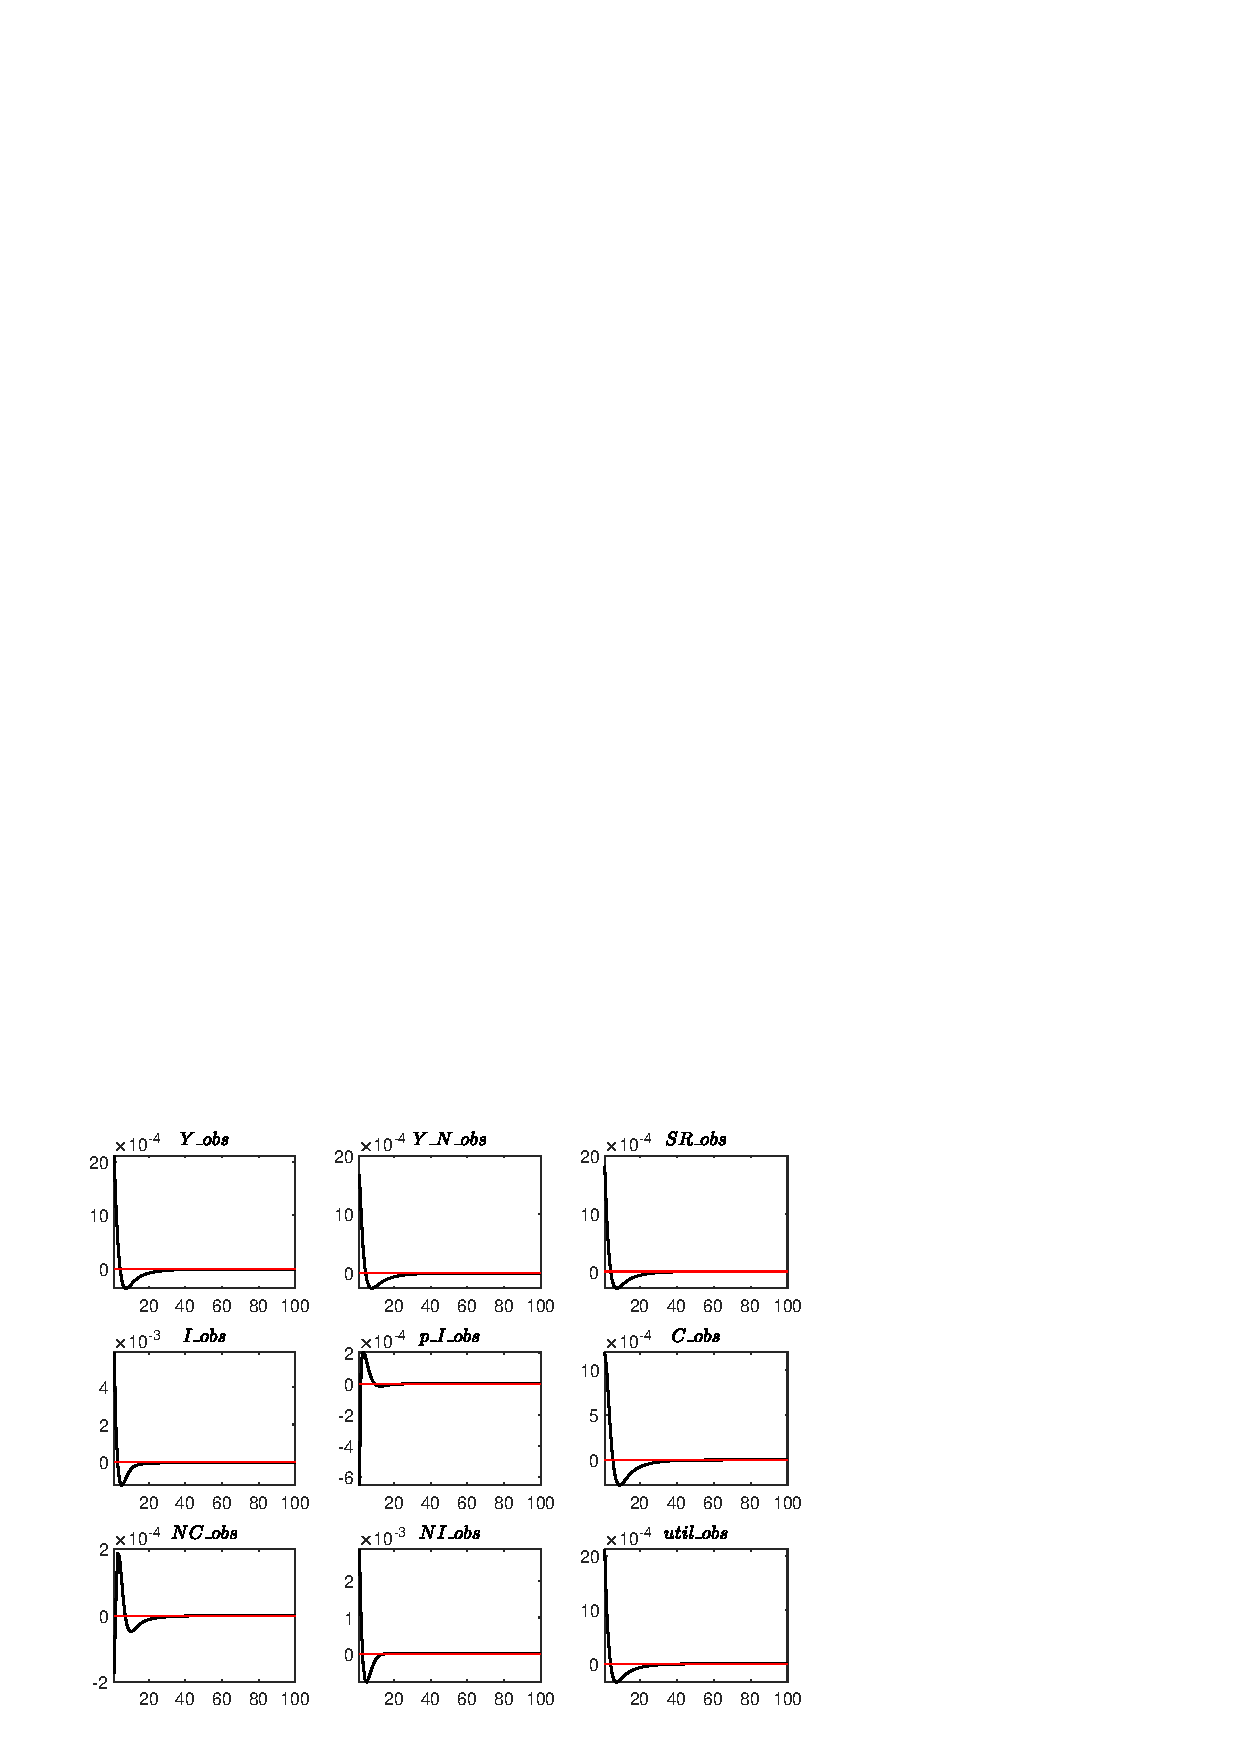
\includegraphics[width=0.80\textwidth]{BRS_sectoral/graphs/BRS_sectoral_IRF_e_D1}
\caption{Impulse response functions (orthogonalized shock to ${e_D}$).}\label{Fig:IRF:e_D:1}
\end{figure}
 
\begin{figure}[H]
\centering 
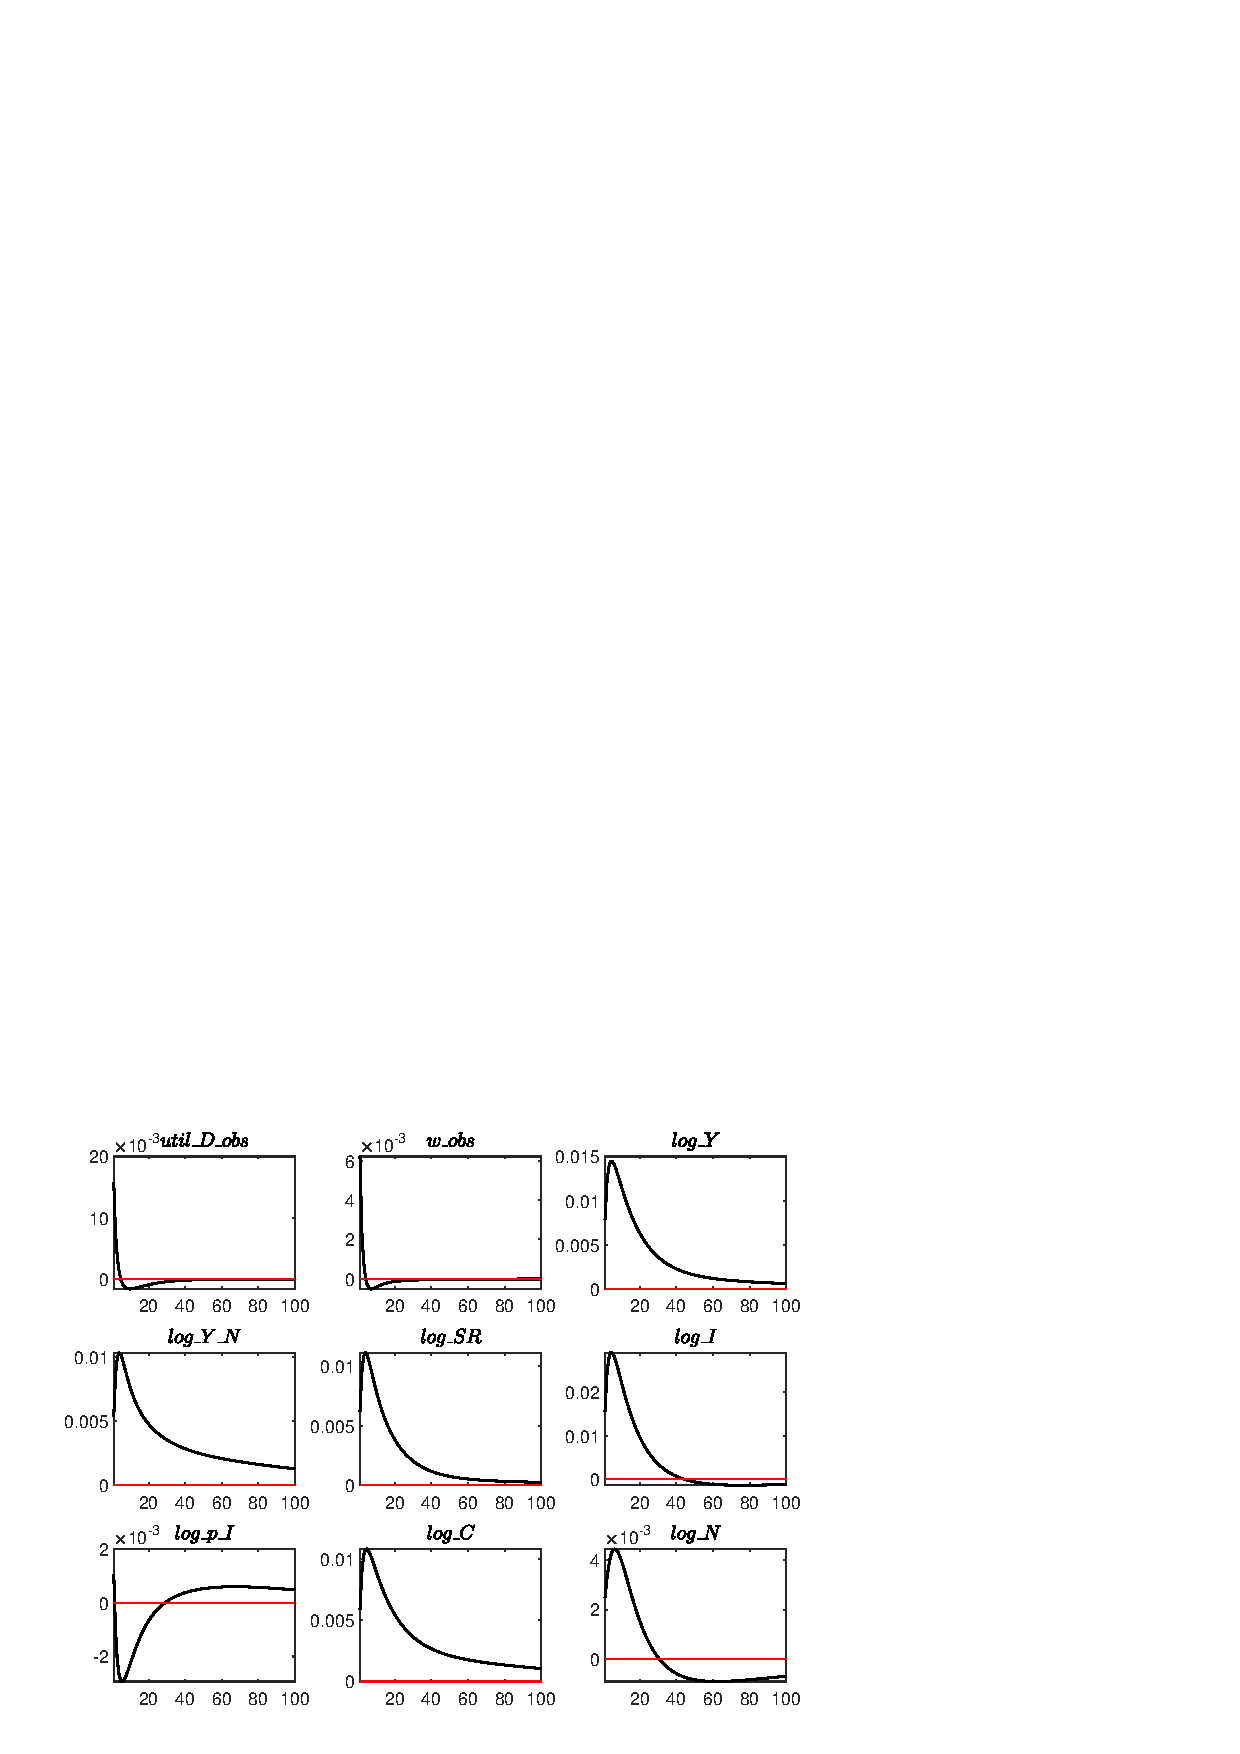
\includegraphics[width=0.80\textwidth]{BRS_sectoral/graphs/BRS_sectoral_IRF_e_D2}
\caption{Impulse response functions (orthogonalized shock to ${e_D}$).}\label{Fig:IRF:e_D:2}
\end{figure}
 
\begin{figure}[H]
\centering 
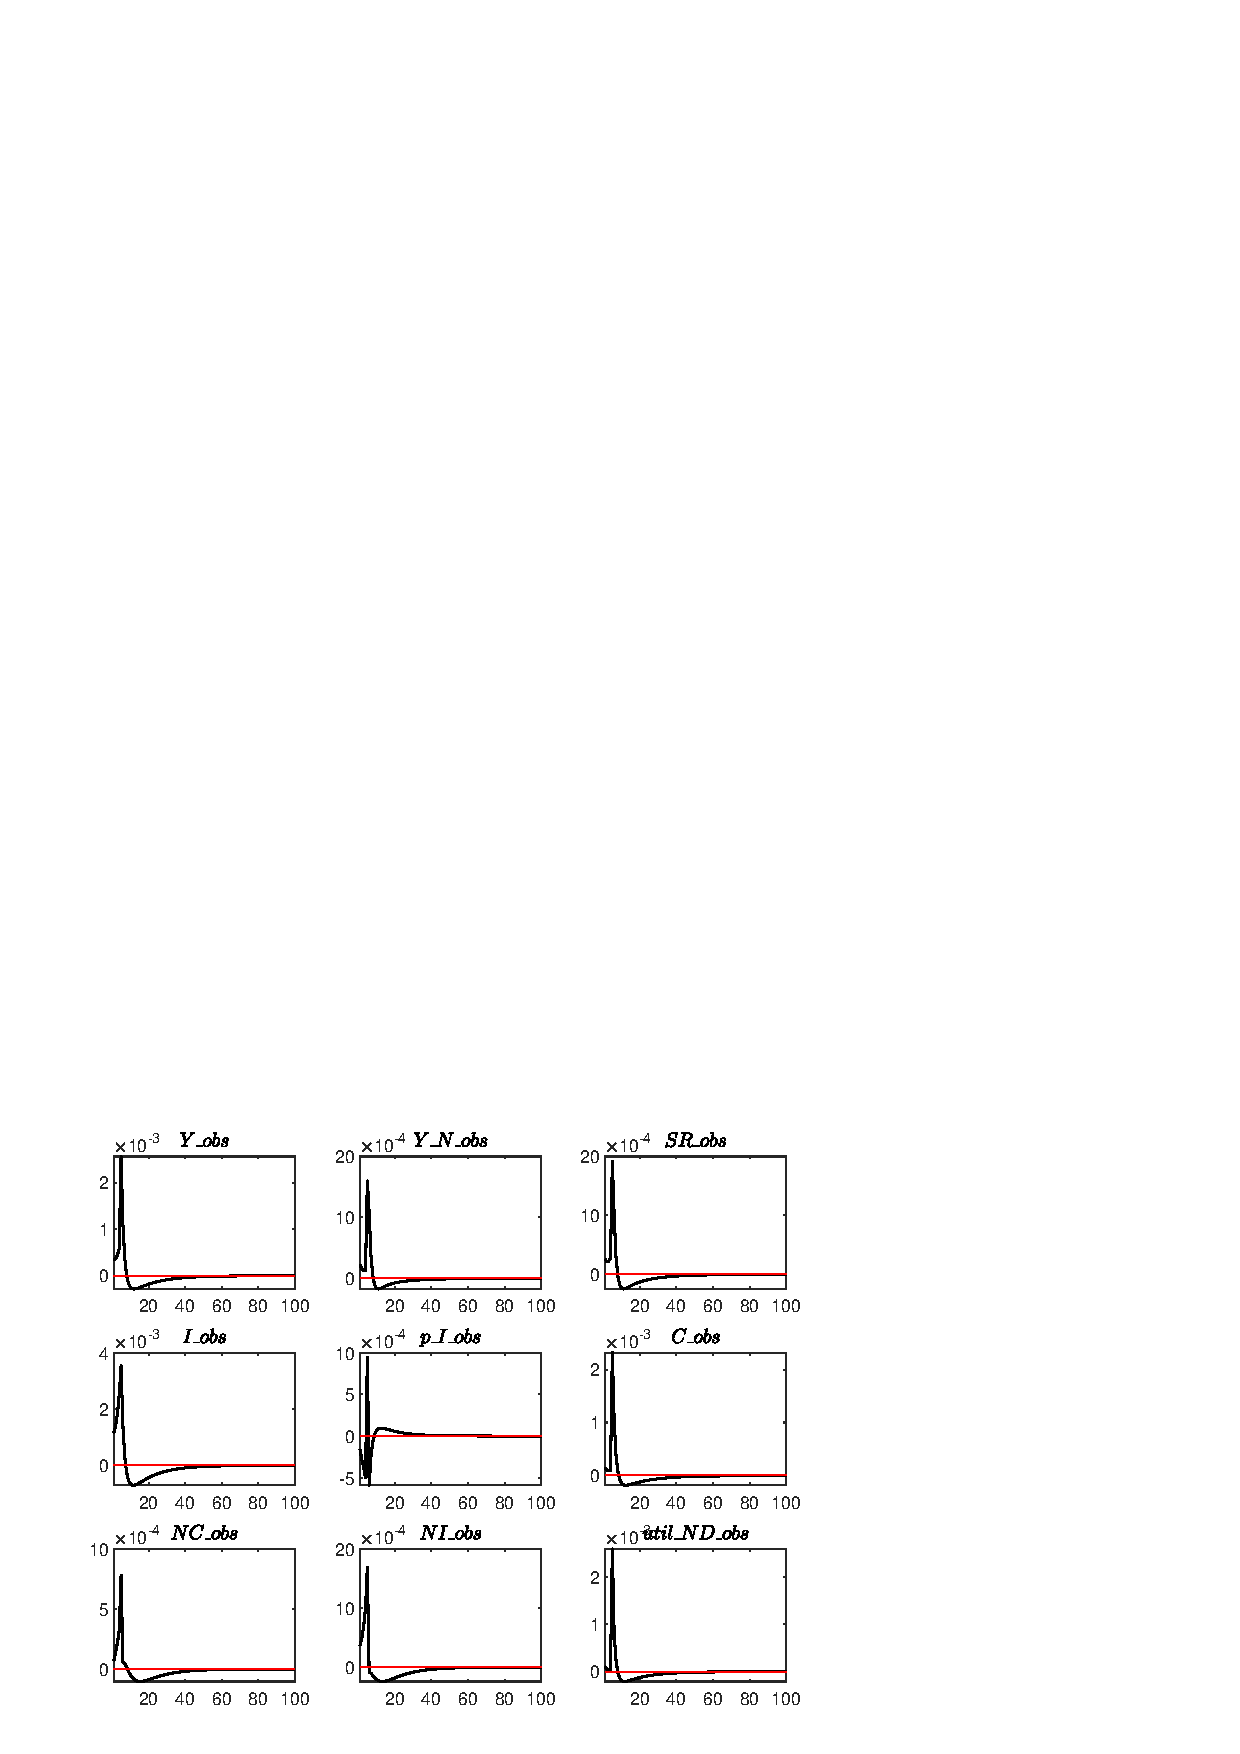
\includegraphics[width=0.80\textwidth]{BRS_sectoral/graphs/BRS_sectoral_IRF_e_D_news1}
\caption{Impulse response functions (orthogonalized shock to ${e_{D,4}}$).}\label{Fig:IRF:e_D_news:1}
\end{figure}
 
\begin{figure}[H]
\centering 
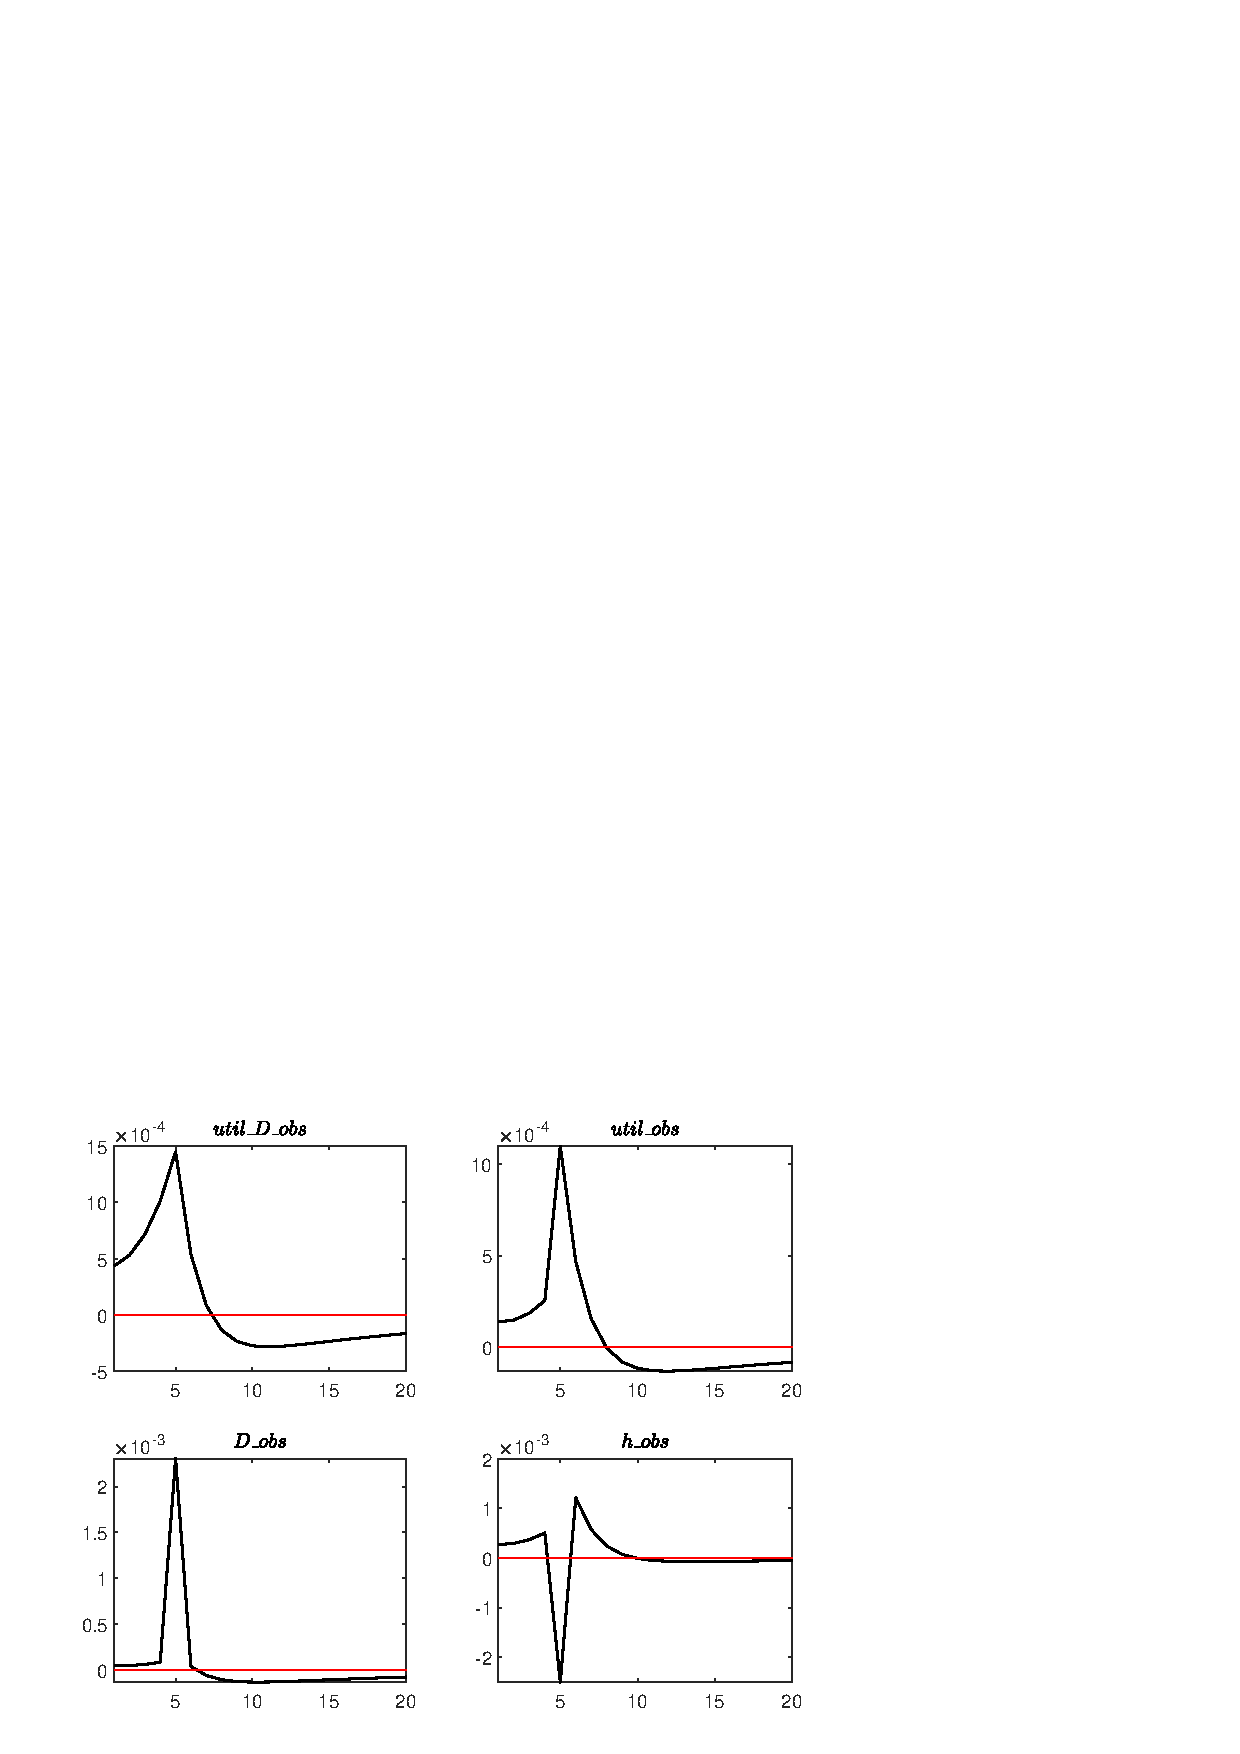
\includegraphics[width=0.80\textwidth]{BRS_sectoral/graphs/BRS_sectoral_IRF_e_D_news2}
\caption{Impulse response functions (orthogonalized shock to ${e_{D,4}}$).}\label{Fig:IRF:e_D_news:2}
\end{figure}
 
\begin{figure}[H]
\centering 
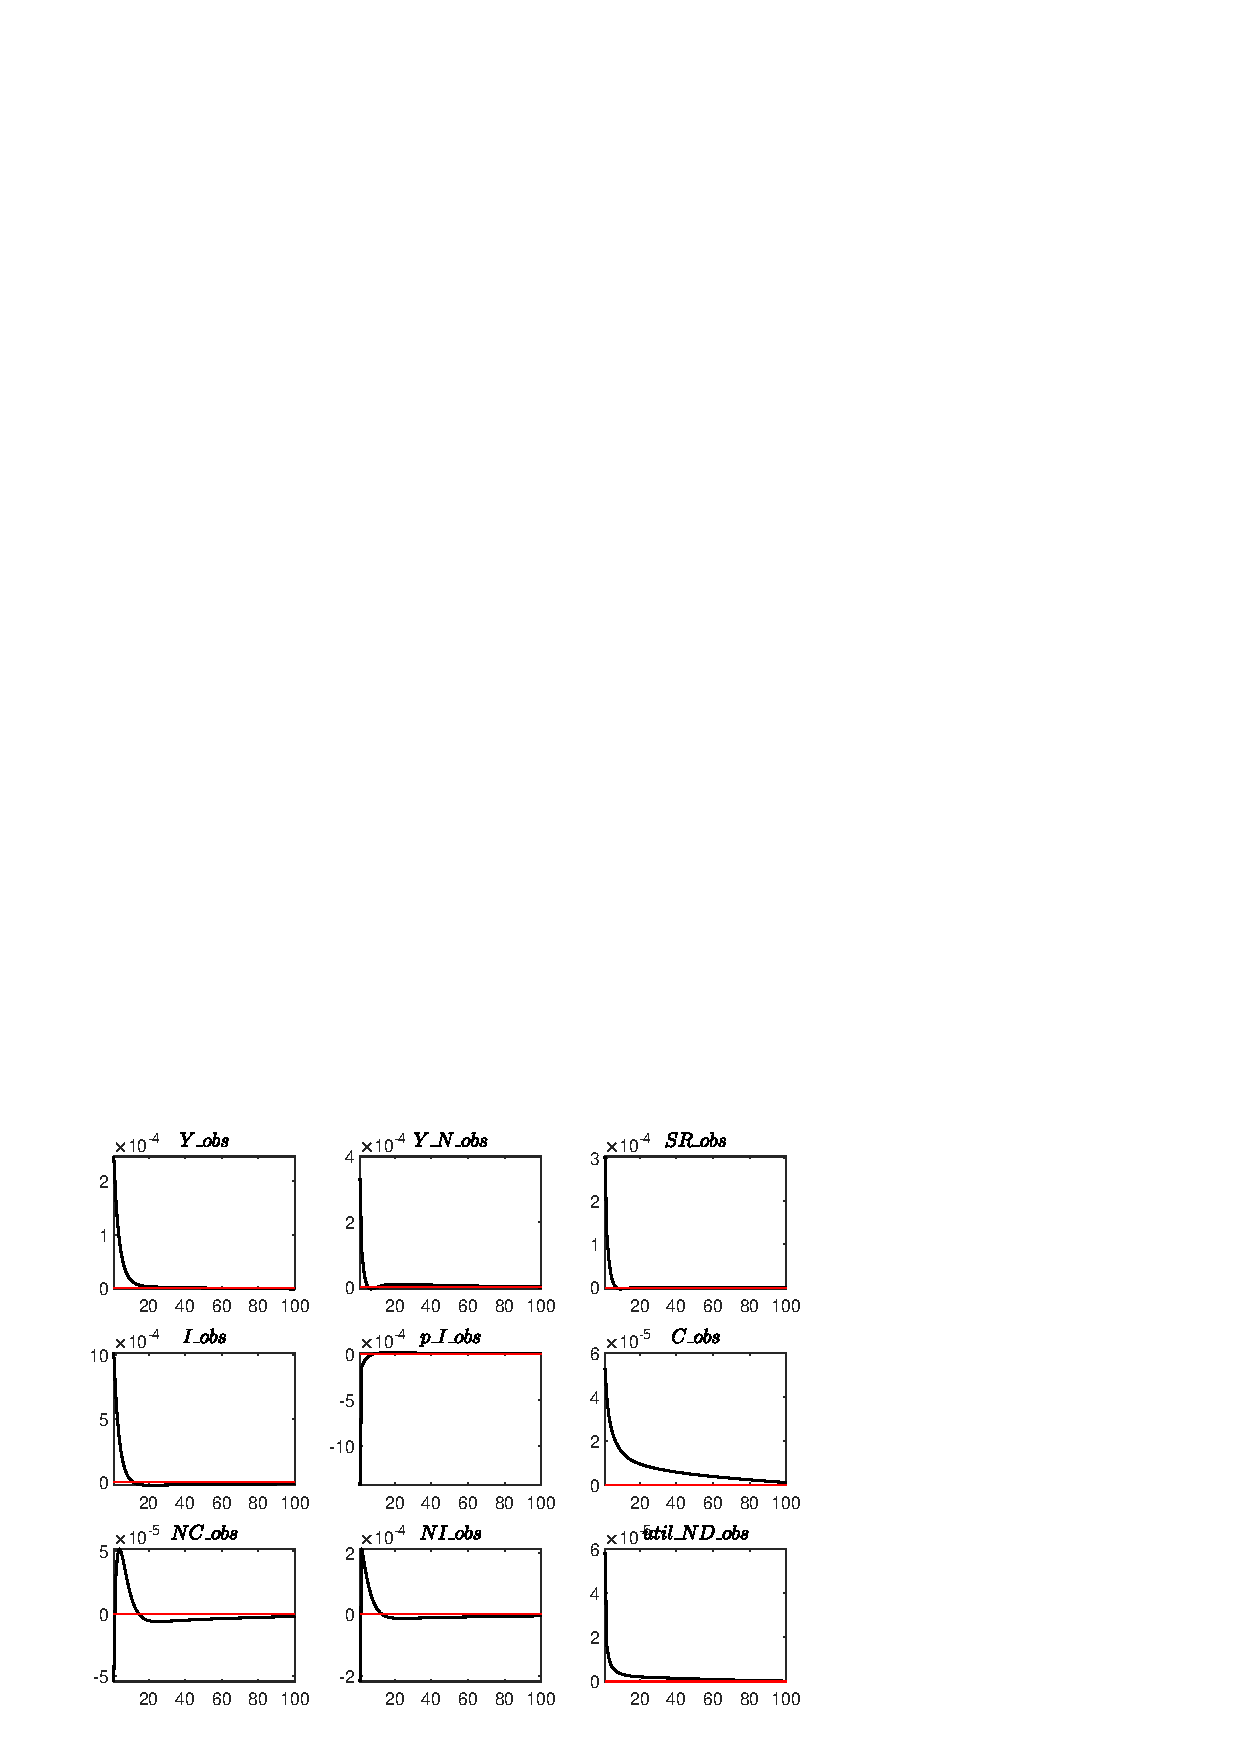
\includegraphics[width=0.80\textwidth]{BRS_sectoral/graphs/BRS_sectoral_IRF_e_DI1}
\caption{Impulse response functions (orthogonalized shock to ${e_DI}$).}\label{Fig:IRF:e_DI:1}
\end{figure}
 
\begin{figure}[H]
\centering 
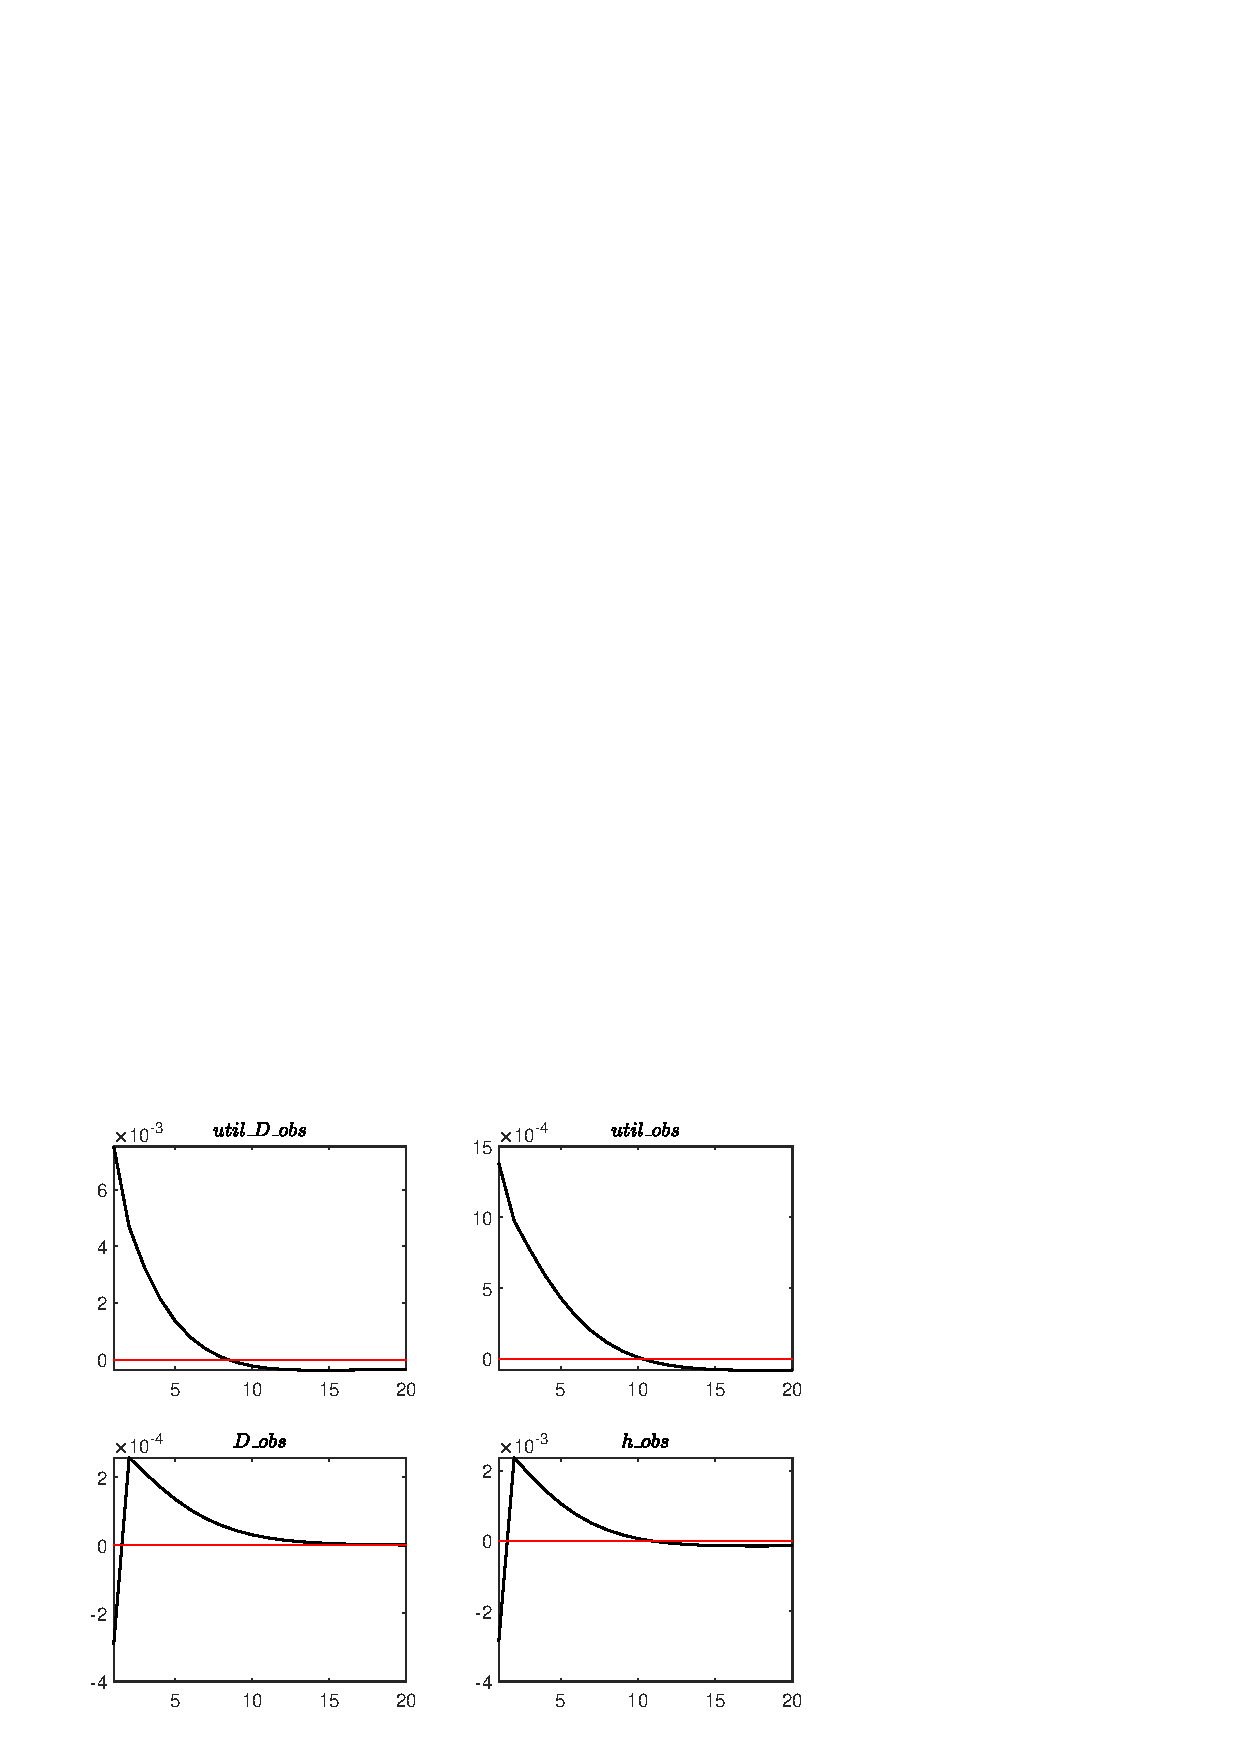
\includegraphics[width=0.80\textwidth]{BRS_sectoral/graphs/BRS_sectoral_IRF_e_DI2}
\caption{Impulse response functions (orthogonalized shock to ${e_DI}$).}\label{Fig:IRF:e_DI:2}
\end{figure}
 
\begin{figure}[H]
\centering 
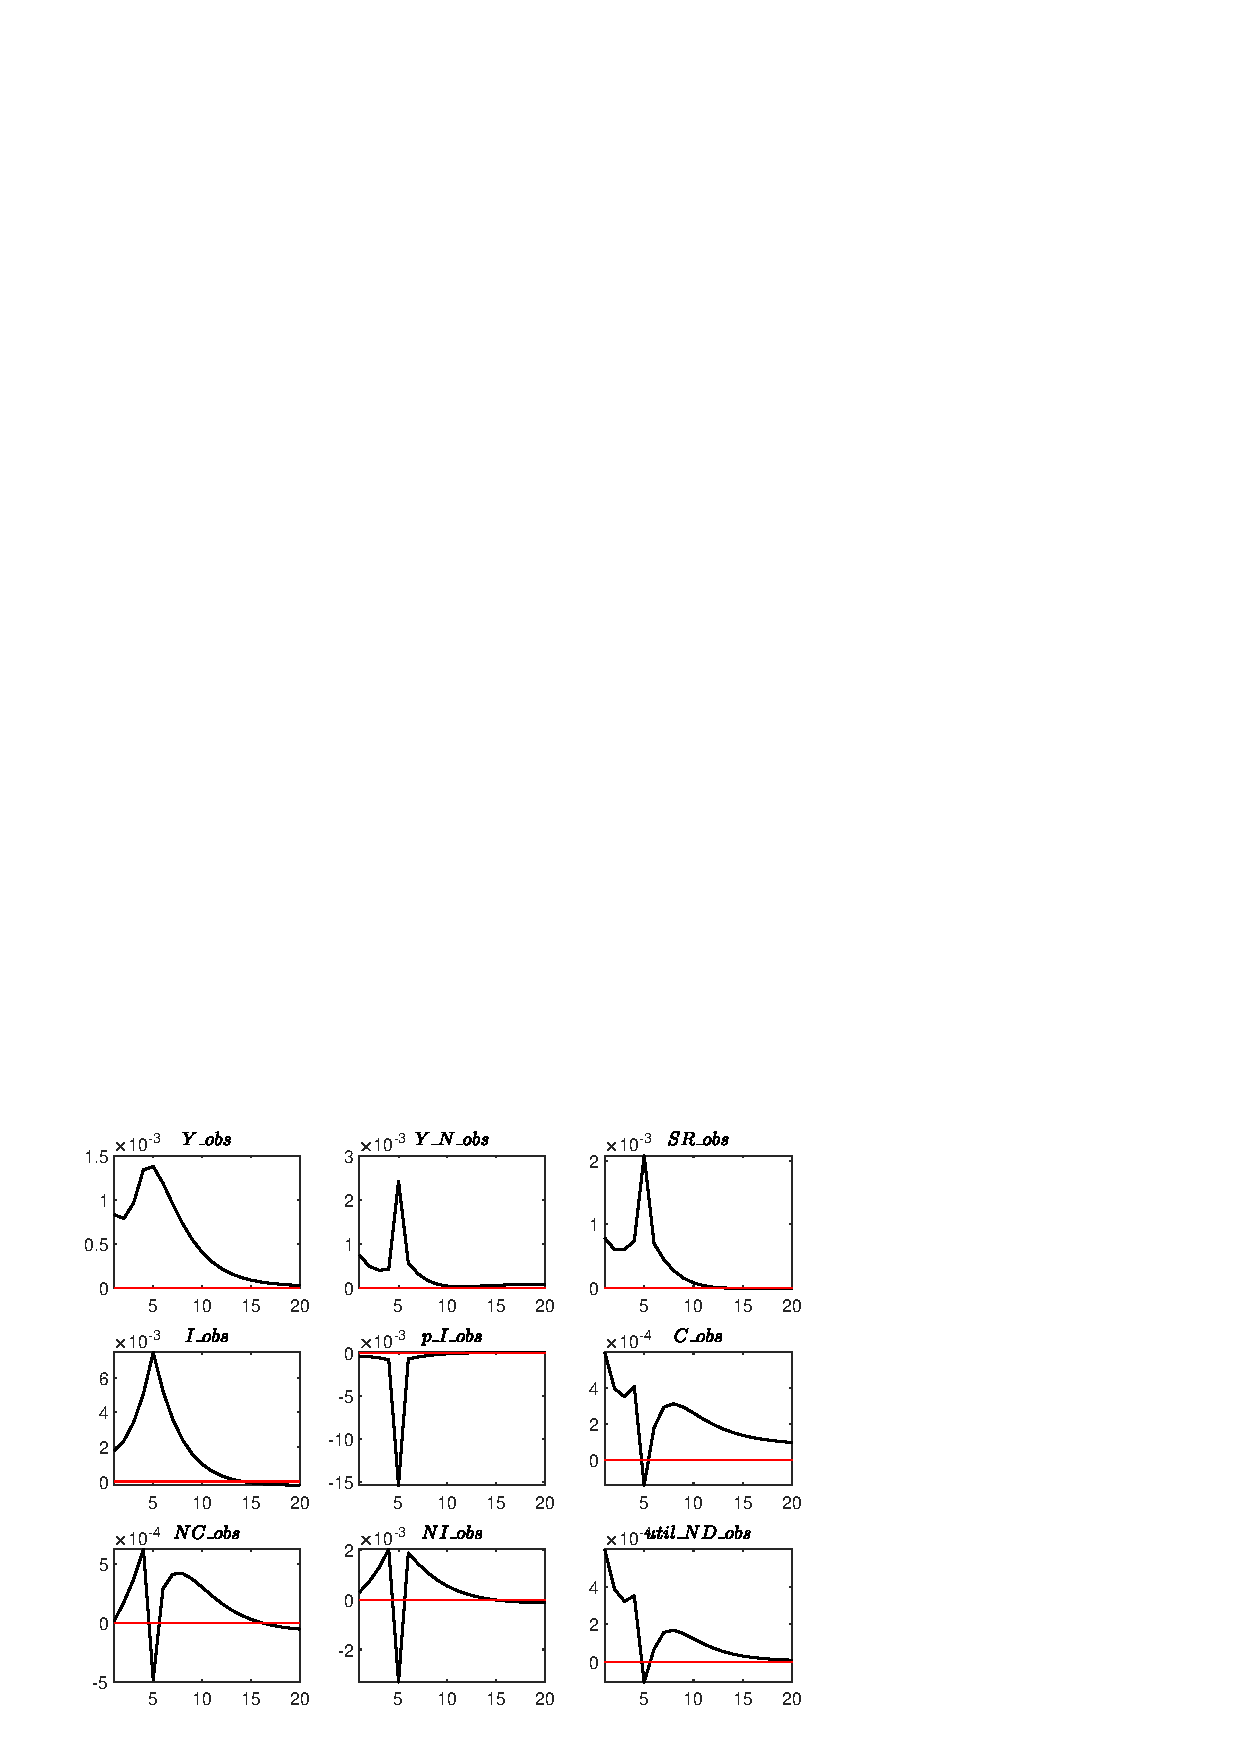
\includegraphics[width=0.80\textwidth]{BRS_sectoral/graphs/BRS_sectoral_IRF_e_DI_news1}
\caption{Impulse response functions (orthogonalized shock to ${e_{DI,-4}}$).}\label{Fig:IRF:e_DI_news:1}
\end{figure}
 
\begin{figure}[H]
\centering 
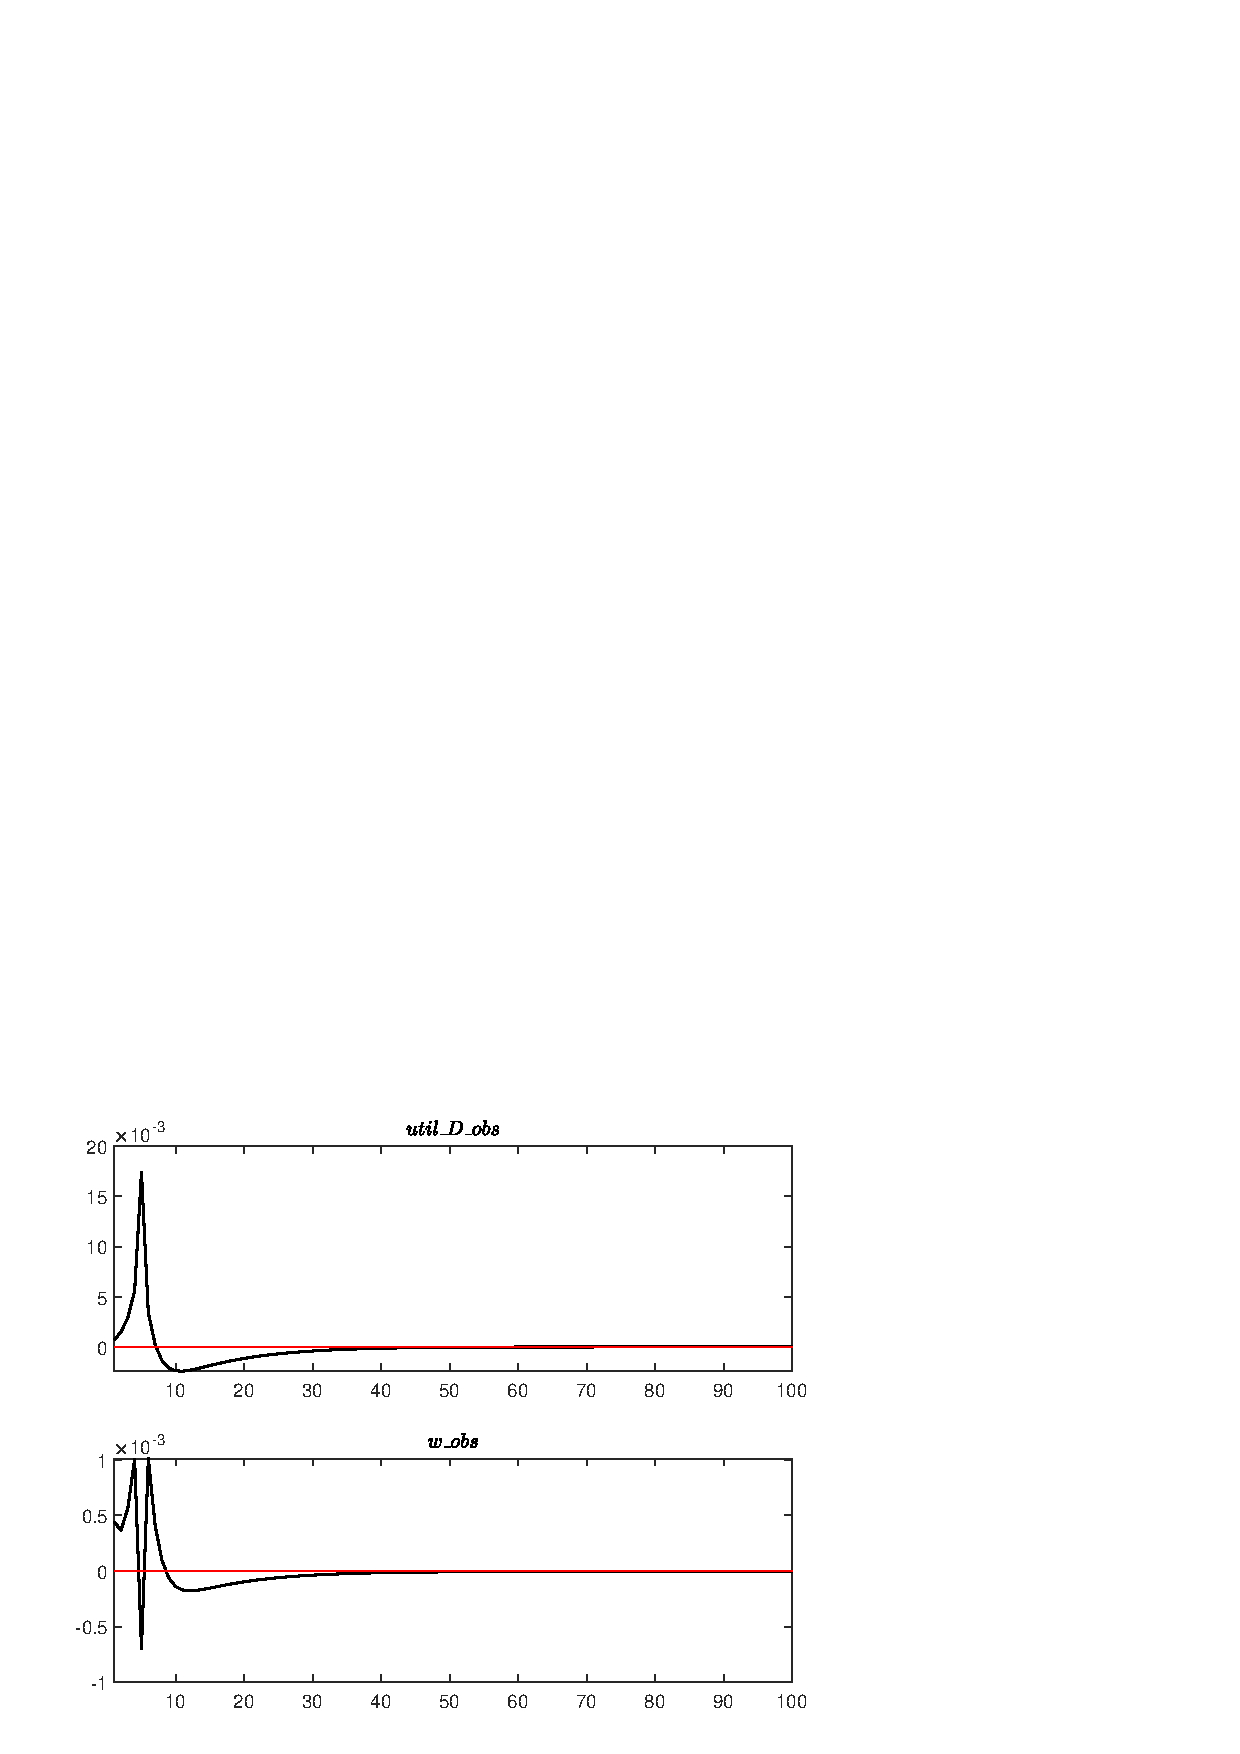
\includegraphics[width=0.80\textwidth]{BRS_sectoral/graphs/BRS_sectoral_IRF_e_DI_news2}
\caption{Impulse response functions (orthogonalized shock to ${e_{DI,-4}}$).}\label{Fig:IRF:e_DI_news:2}
\end{figure}
 
\begin{figure}[H]
\centering 
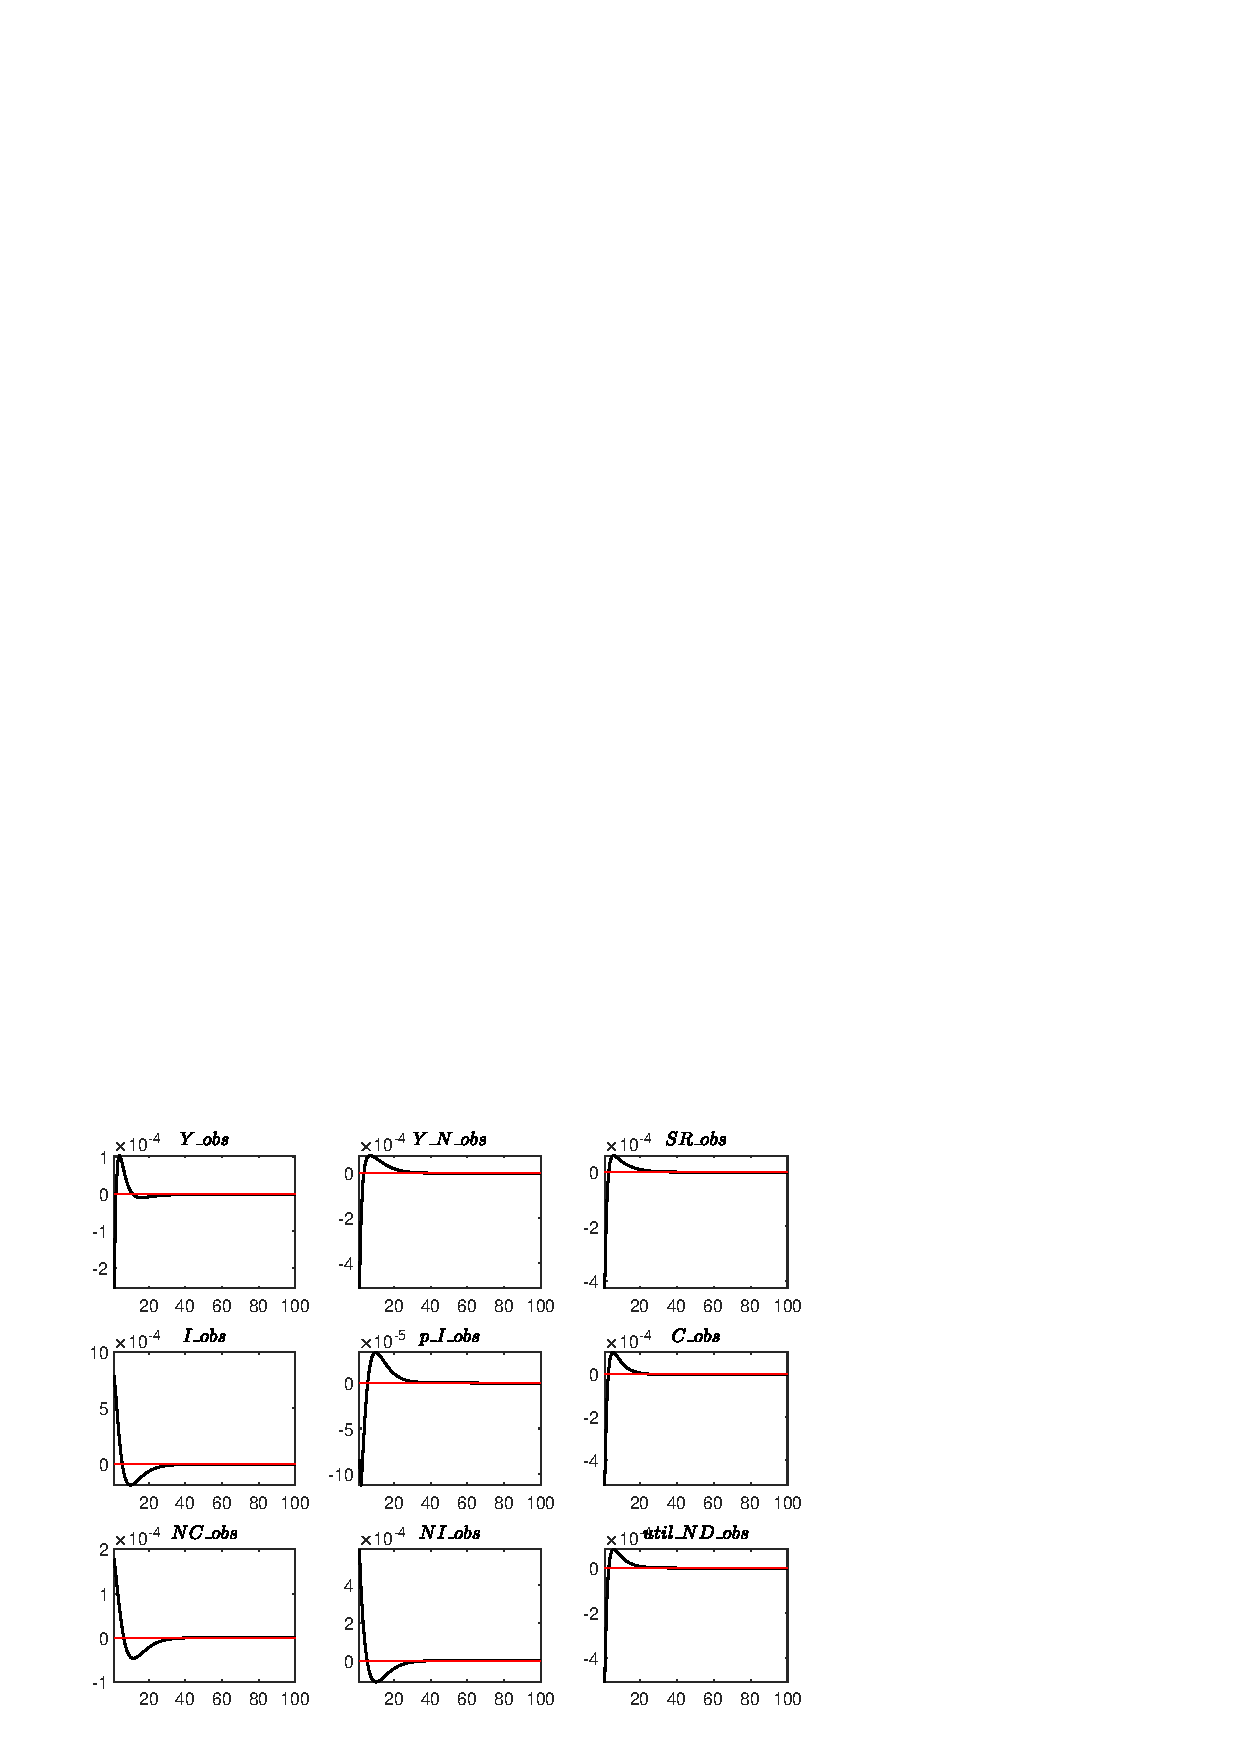
\includegraphics[width=0.80\textwidth]{BRS_sectoral/graphs/BRS_sectoral_IRF_e_b1}
\caption{Impulse response functions (orthogonalized shock to ${e_b}$).}\label{Fig:IRF:e_b:1}
\end{figure}
 
\begin{figure}[H]
\centering 
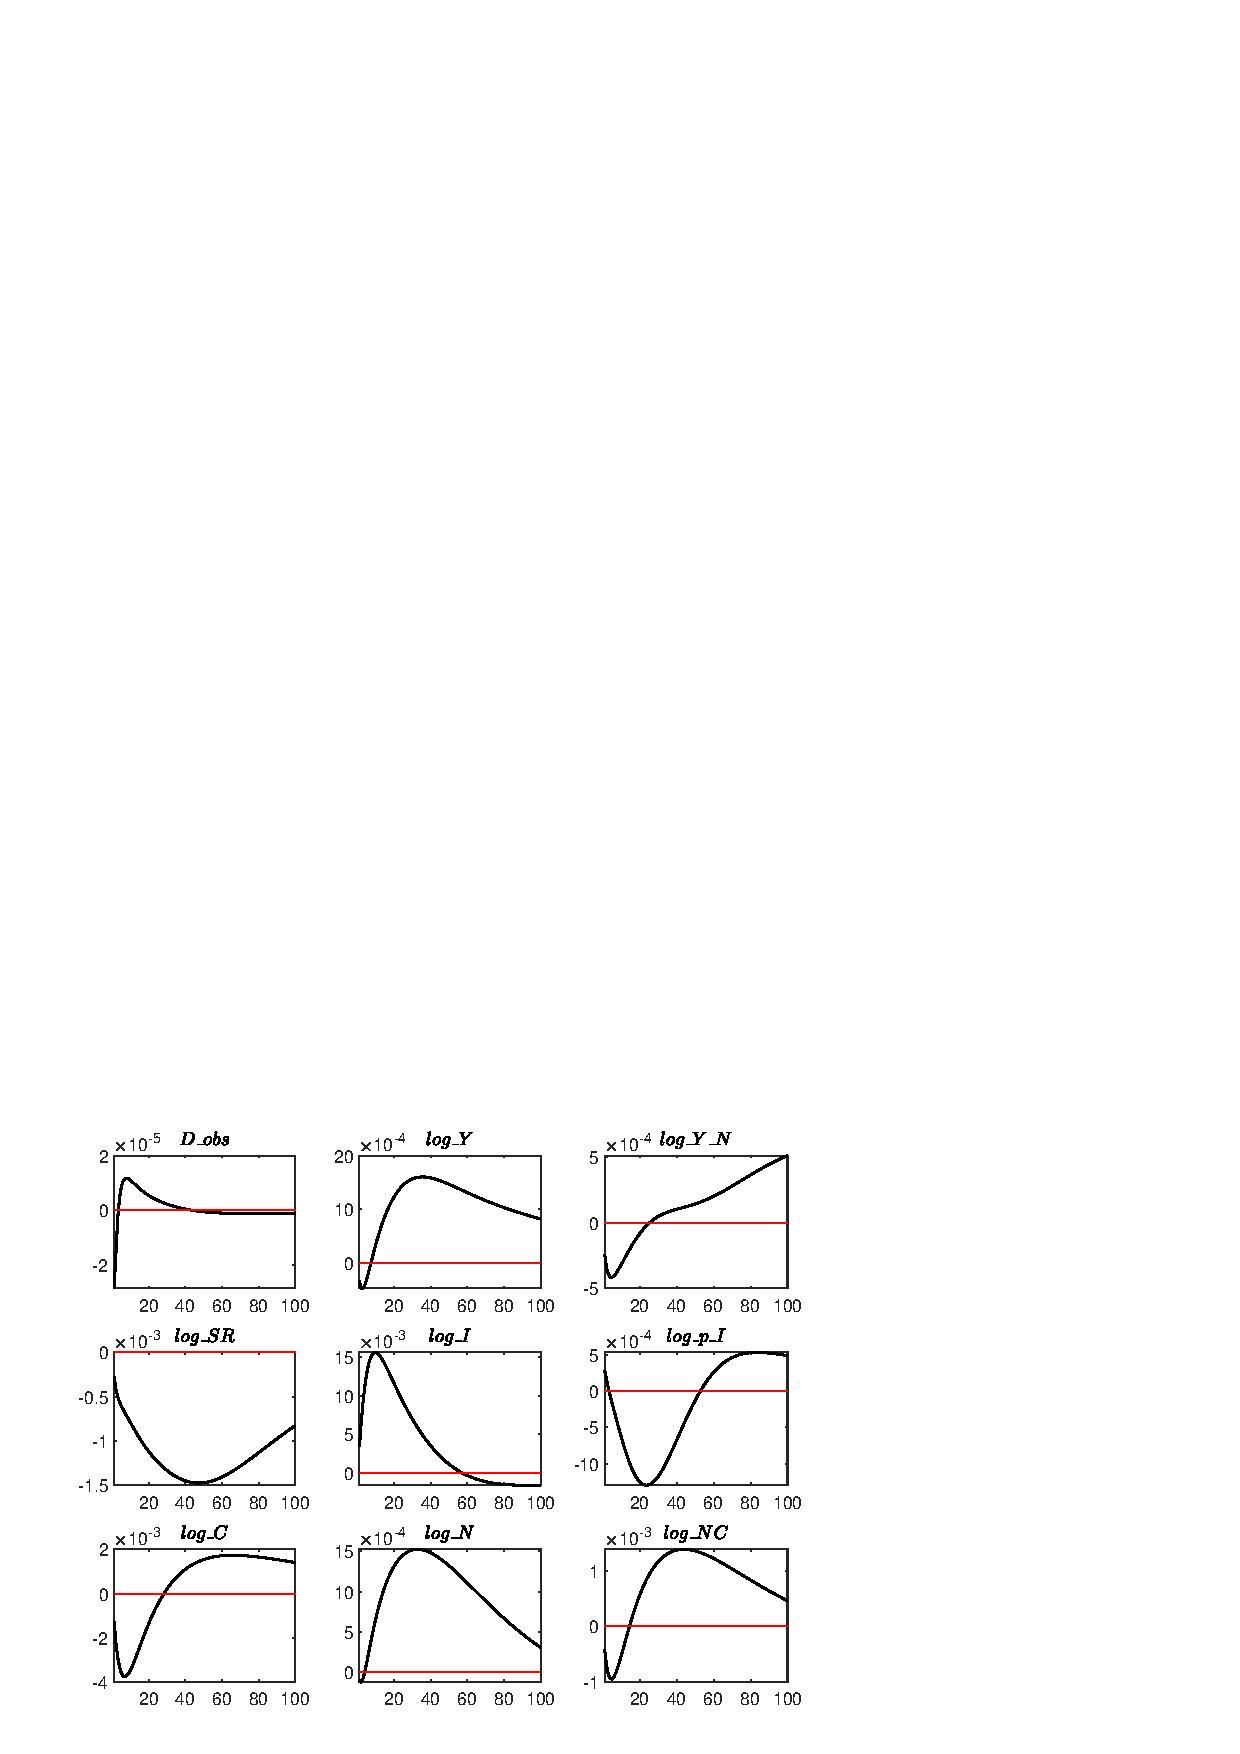
\includegraphics[width=0.80\textwidth]{BRS_sectoral/graphs/BRS_sectoral_IRF_e_b2}
\caption{Impulse response functions (orthogonalized shock to ${e_b}$).}\label{Fig:IRF:e_b:2}
\end{figure}
 
\begin{figure}[H]
\centering 
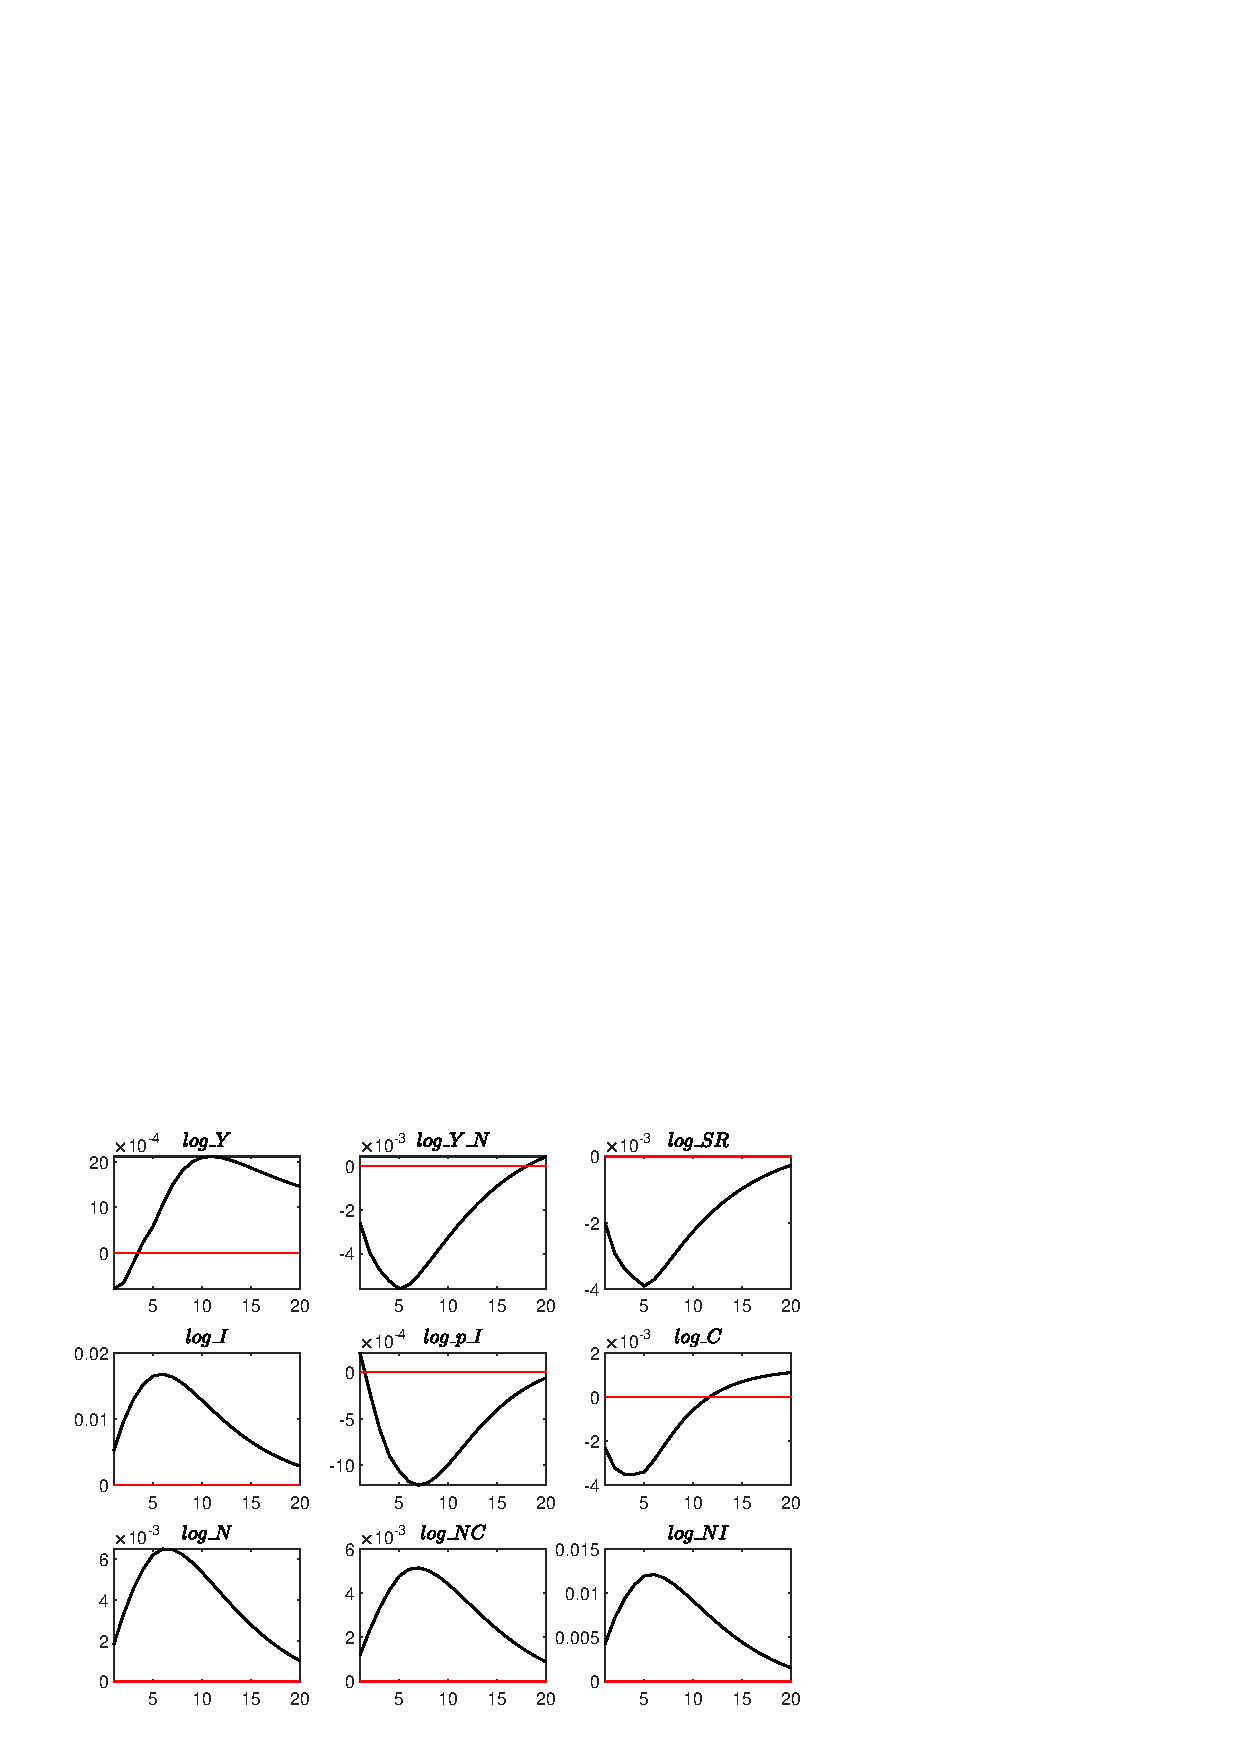
\includegraphics[width=0.80\textwidth]{BRS_sectoral/graphs/BRS_sectoral_IRF_e_b_news1}
\caption{Impulse response functions (orthogonalized shock to ${e_{b,-4}}$).}\label{Fig:IRF:e_b_news:1}
\end{figure}
 
\begin{figure}[H]
\centering 
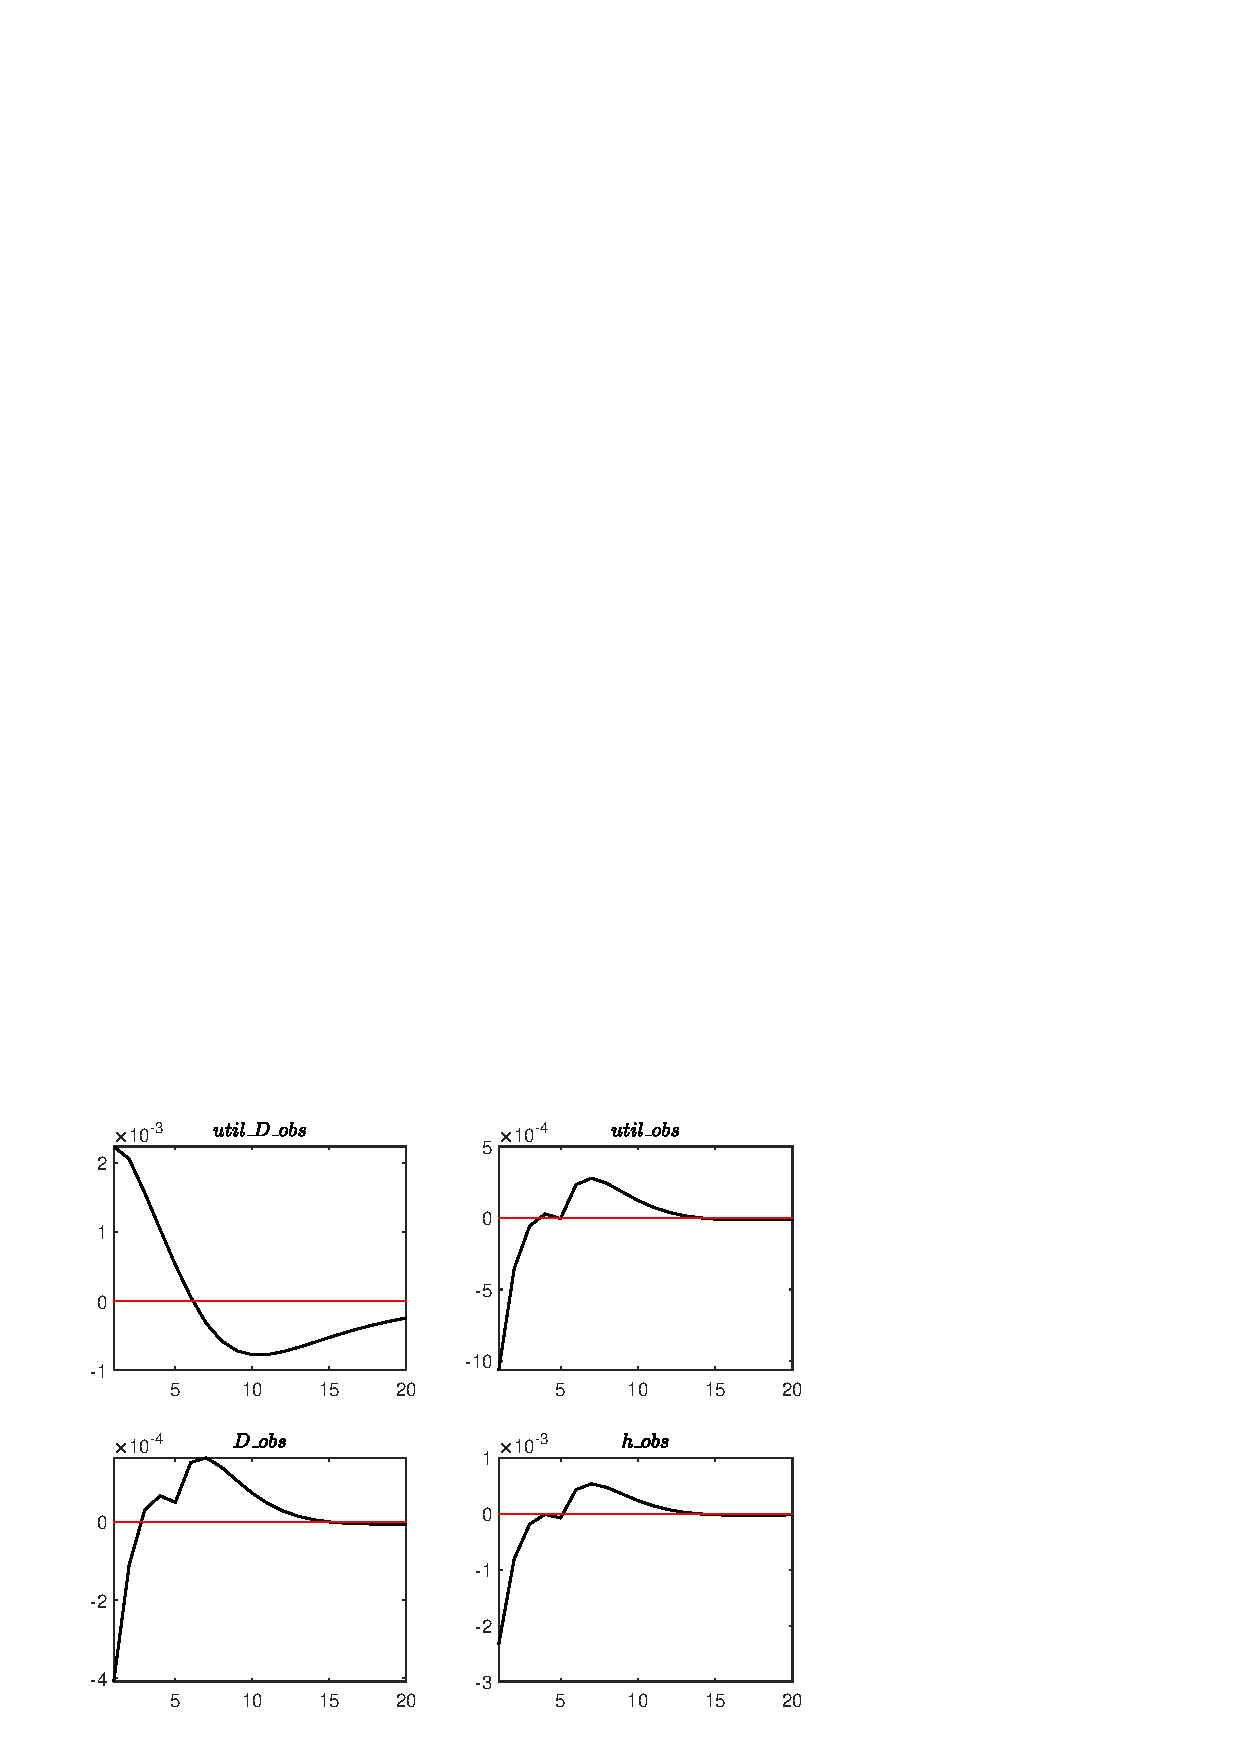
\includegraphics[width=0.80\textwidth]{BRS_sectoral/graphs/BRS_sectoral_IRF_e_b_news2}
\caption{Impulse response functions (orthogonalized shock to ${e_{b,-4}}$).}\label{Fig:IRF:e_b_news:2}
\end{figure}
 
\begin{figure}[H]
\centering 
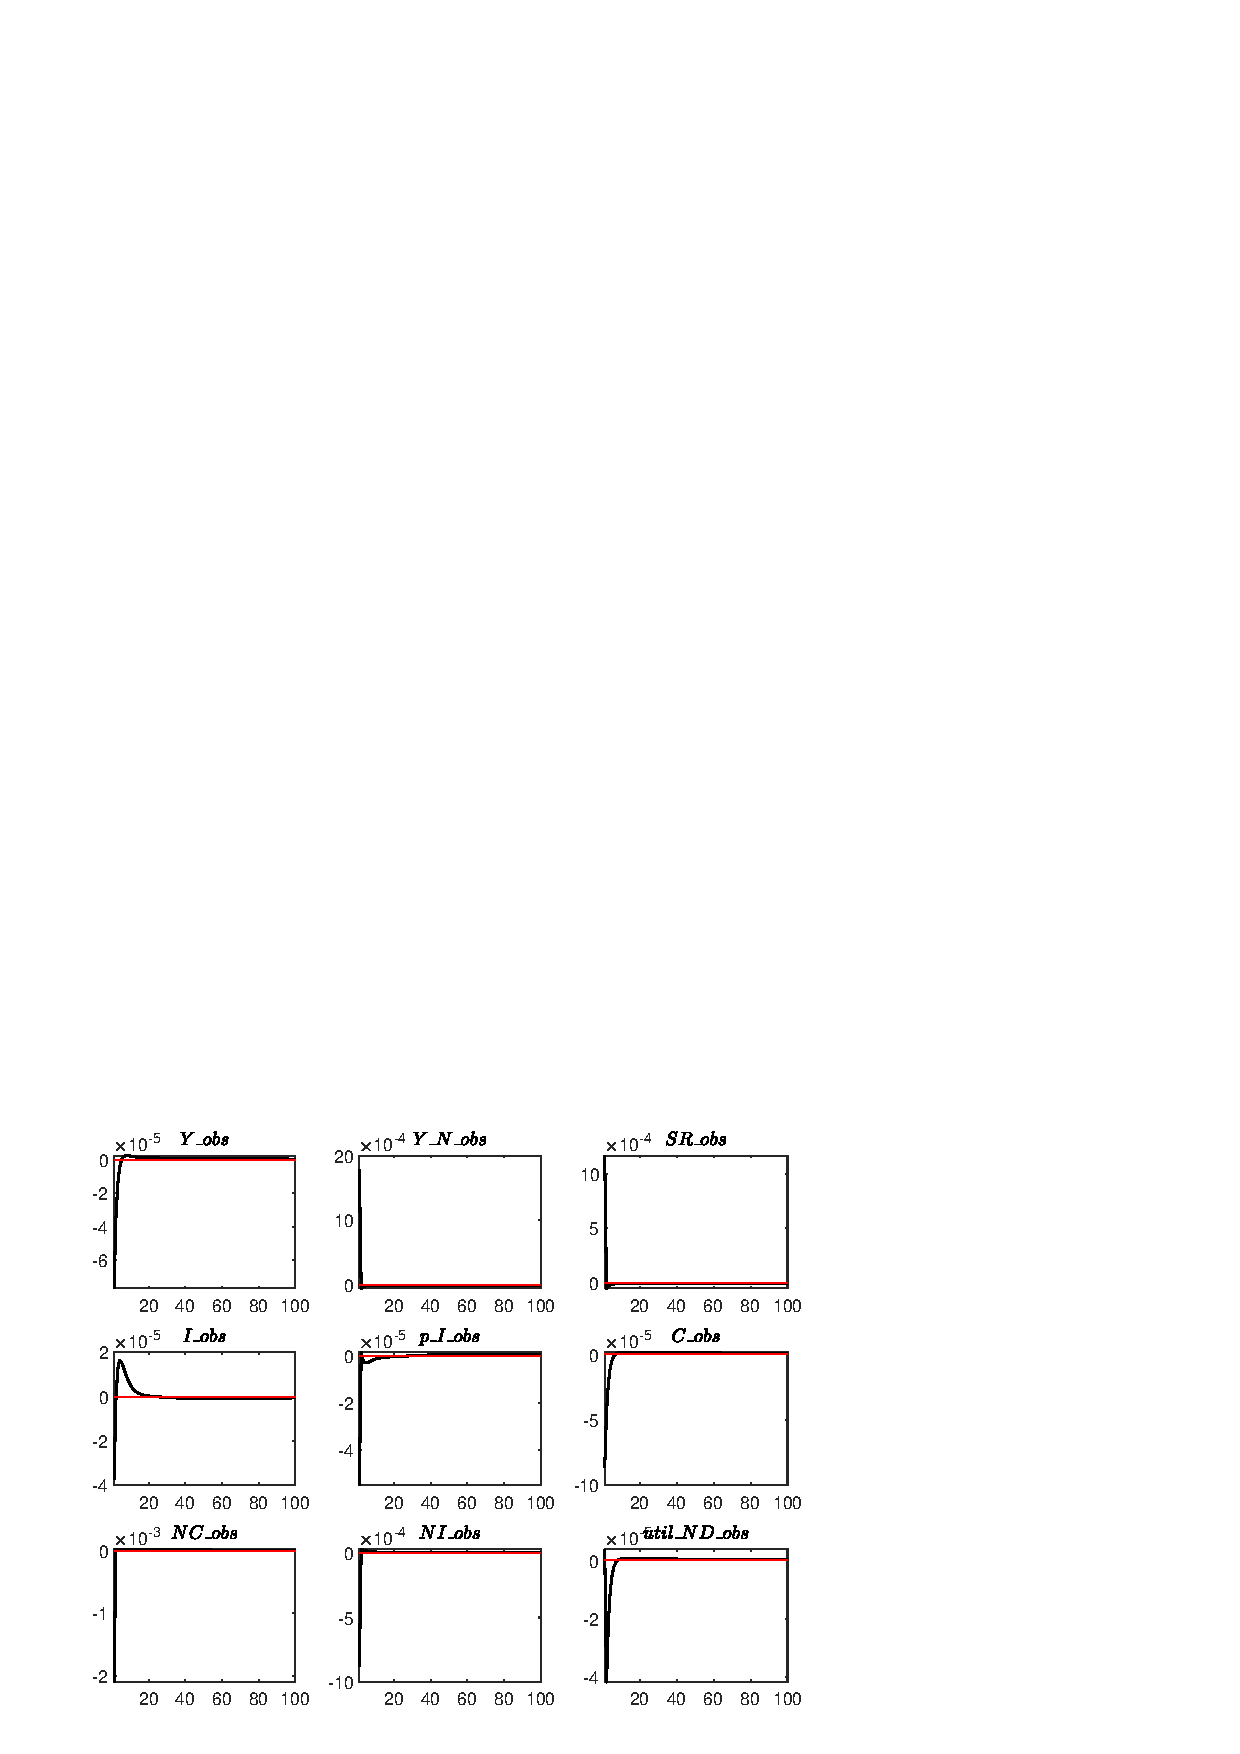
\includegraphics[width=0.80\textwidth]{BRS_sectoral/graphs/BRS_sectoral_IRF_e_muC1}
\caption{Impulse response functions (orthogonalized shock to ${e_{muC}}$).}\label{Fig:IRF:e_muC:1}
\end{figure}
 
\begin{figure}[H]
\centering 
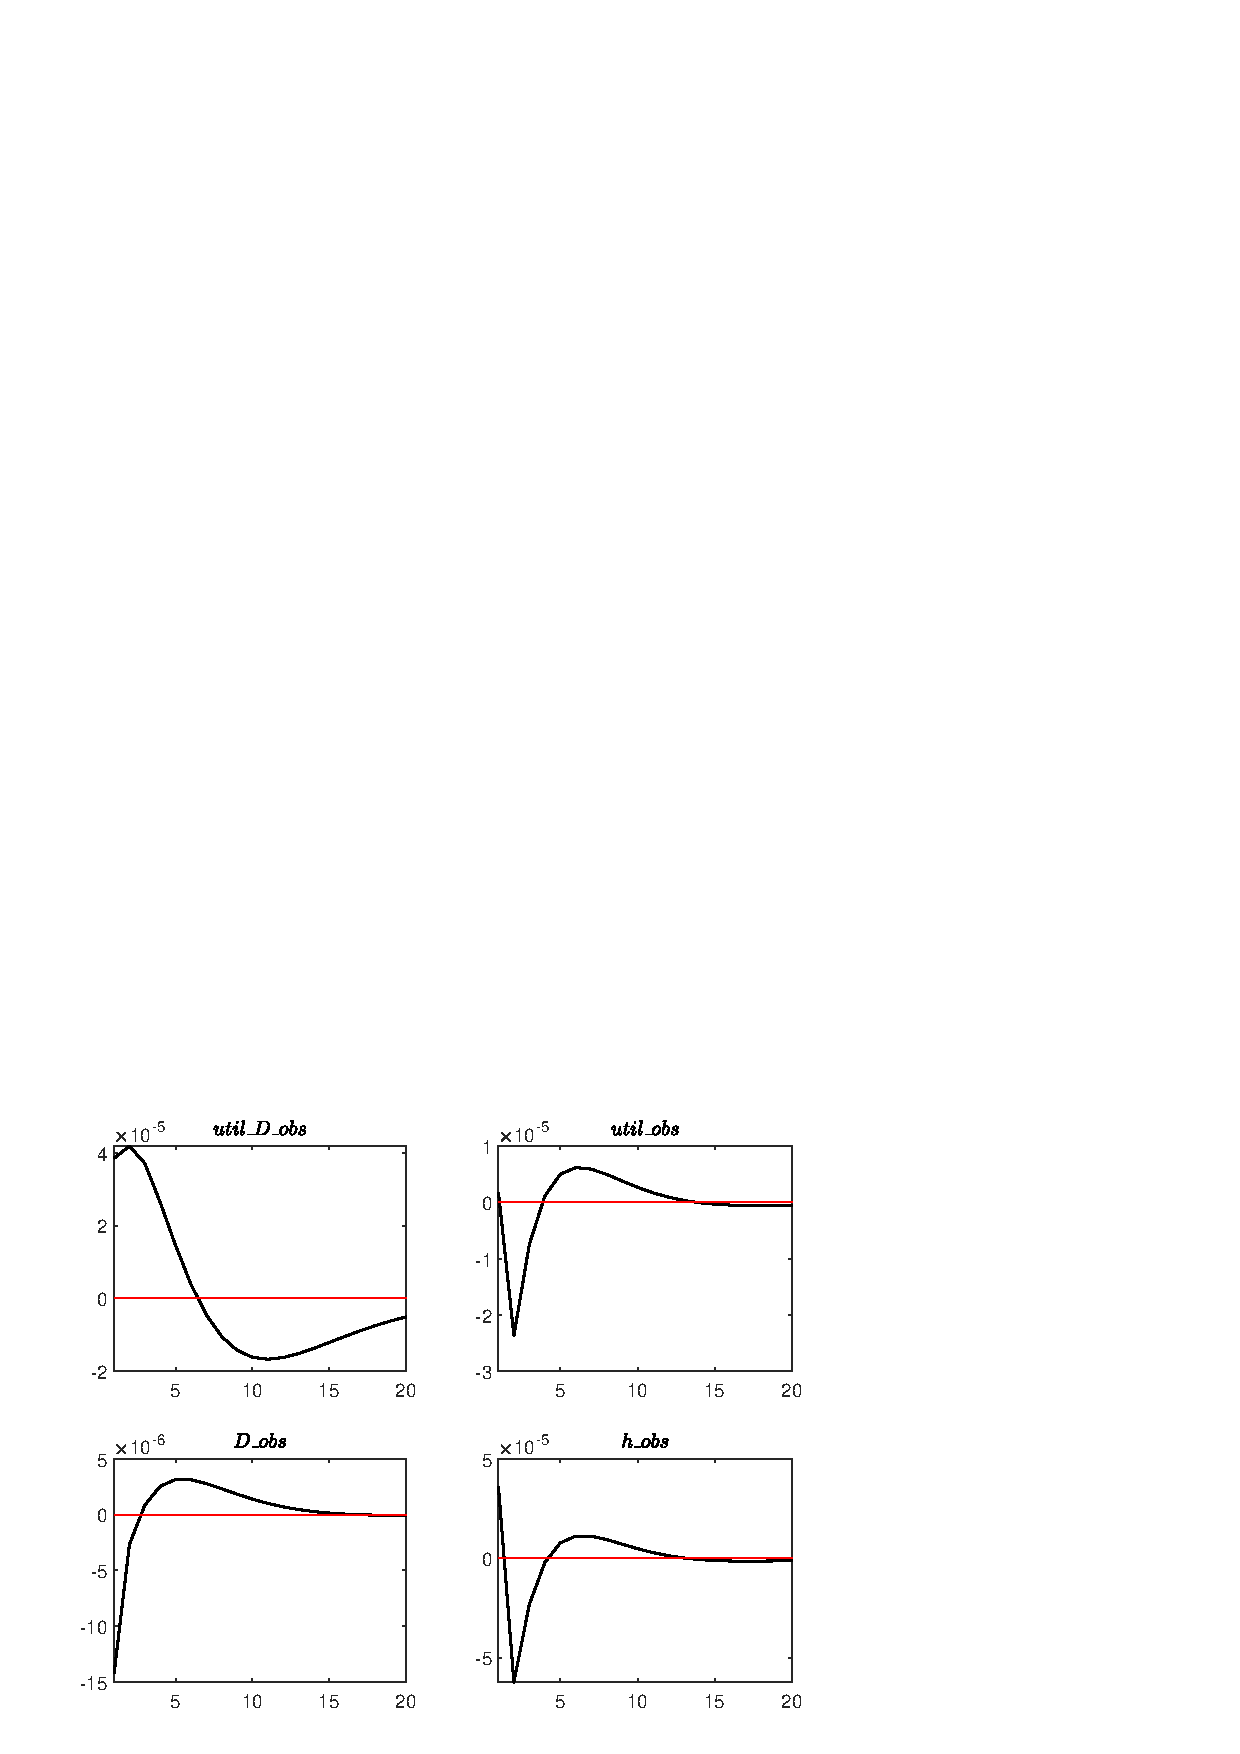
\includegraphics[width=0.80\textwidth]{BRS_sectoral/graphs/BRS_sectoral_IRF_e_muC2}
\caption{Impulse response functions (orthogonalized shock to ${e_{muC}}$).}\label{Fig:IRF:e_muC:2}
\end{figure}
 
\begin{figure}[H]
\centering 
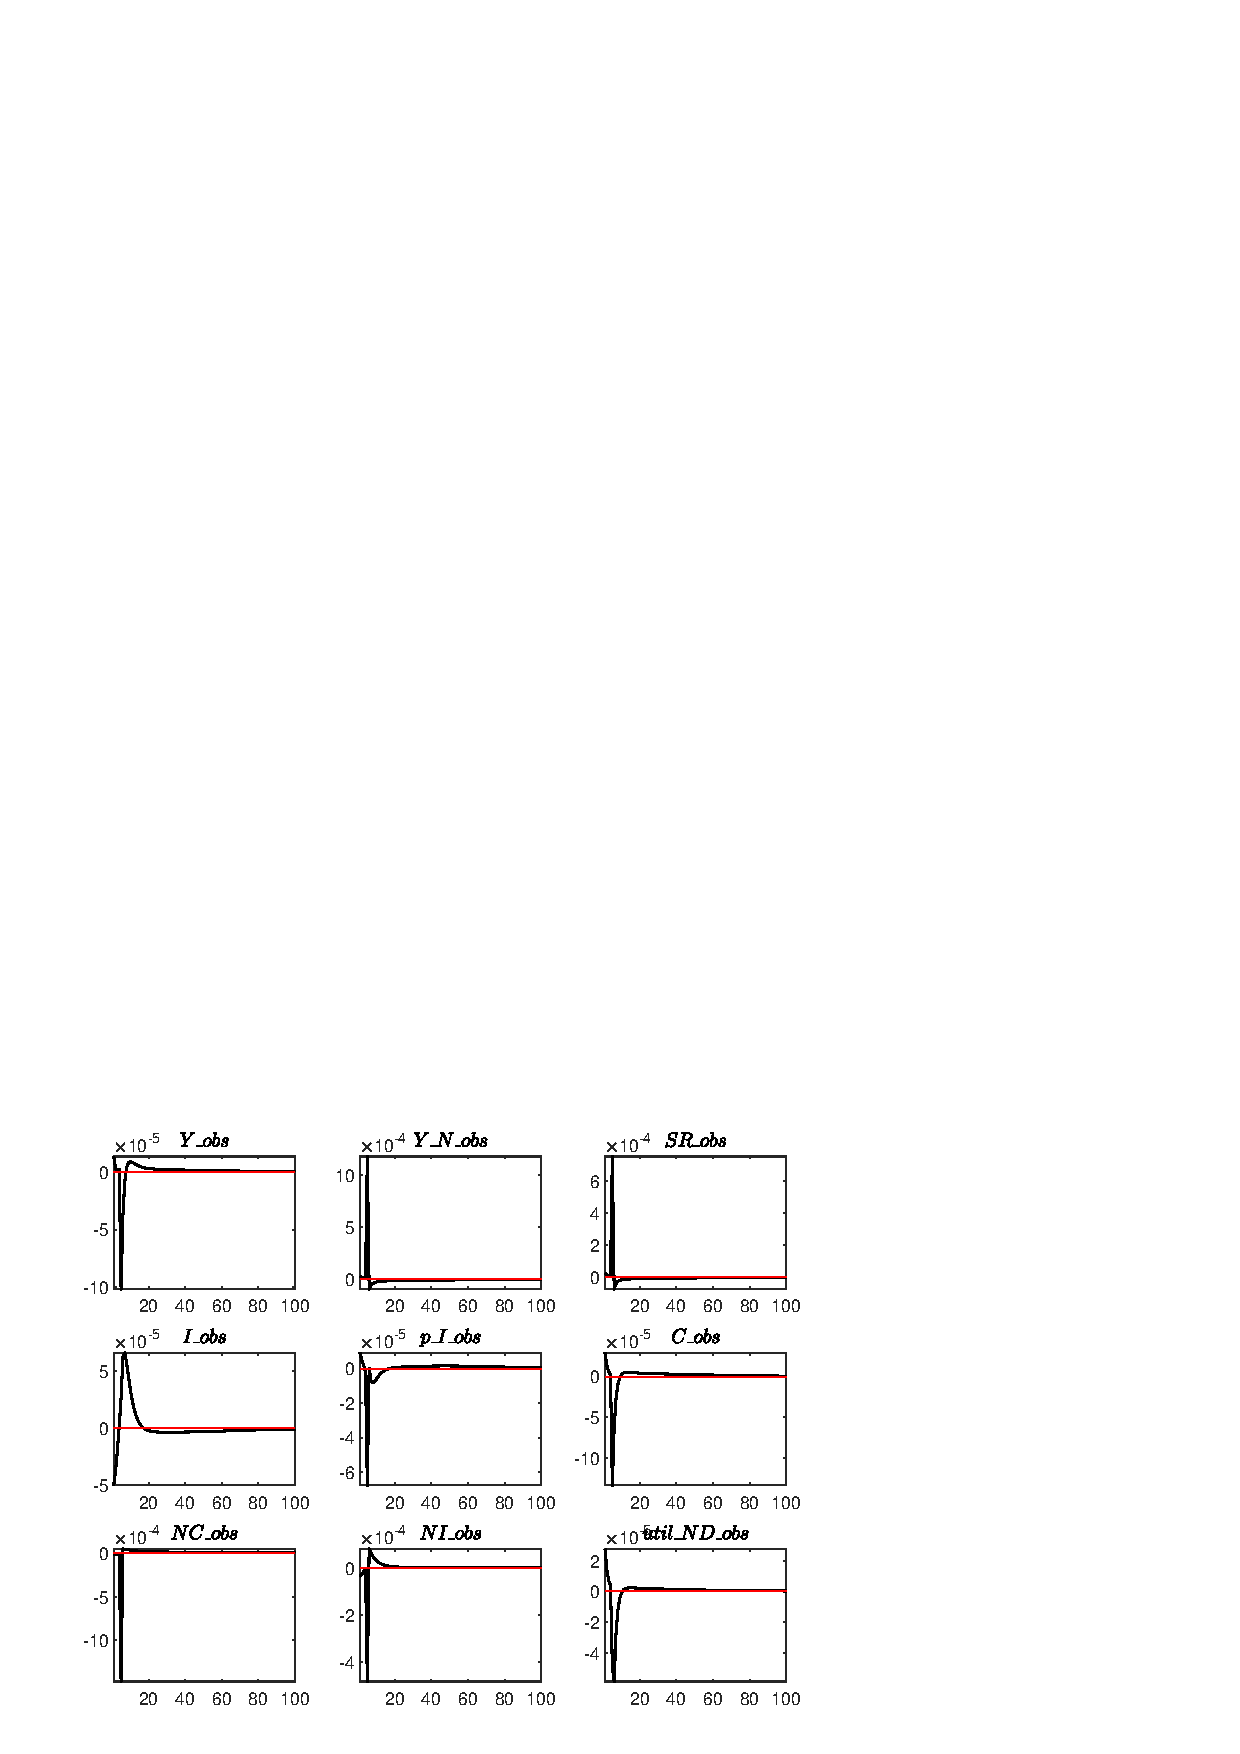
\includegraphics[width=0.80\textwidth]{BRS_sectoral/graphs/BRS_sectoral_IRF_e_muC_news1}
\caption{Impulse response functions (orthogonalized shock to ${e_{muC,-4}}$).}\label{Fig:IRF:e_muC_news:1}
\end{figure}
 
\begin{figure}[H]
\centering 
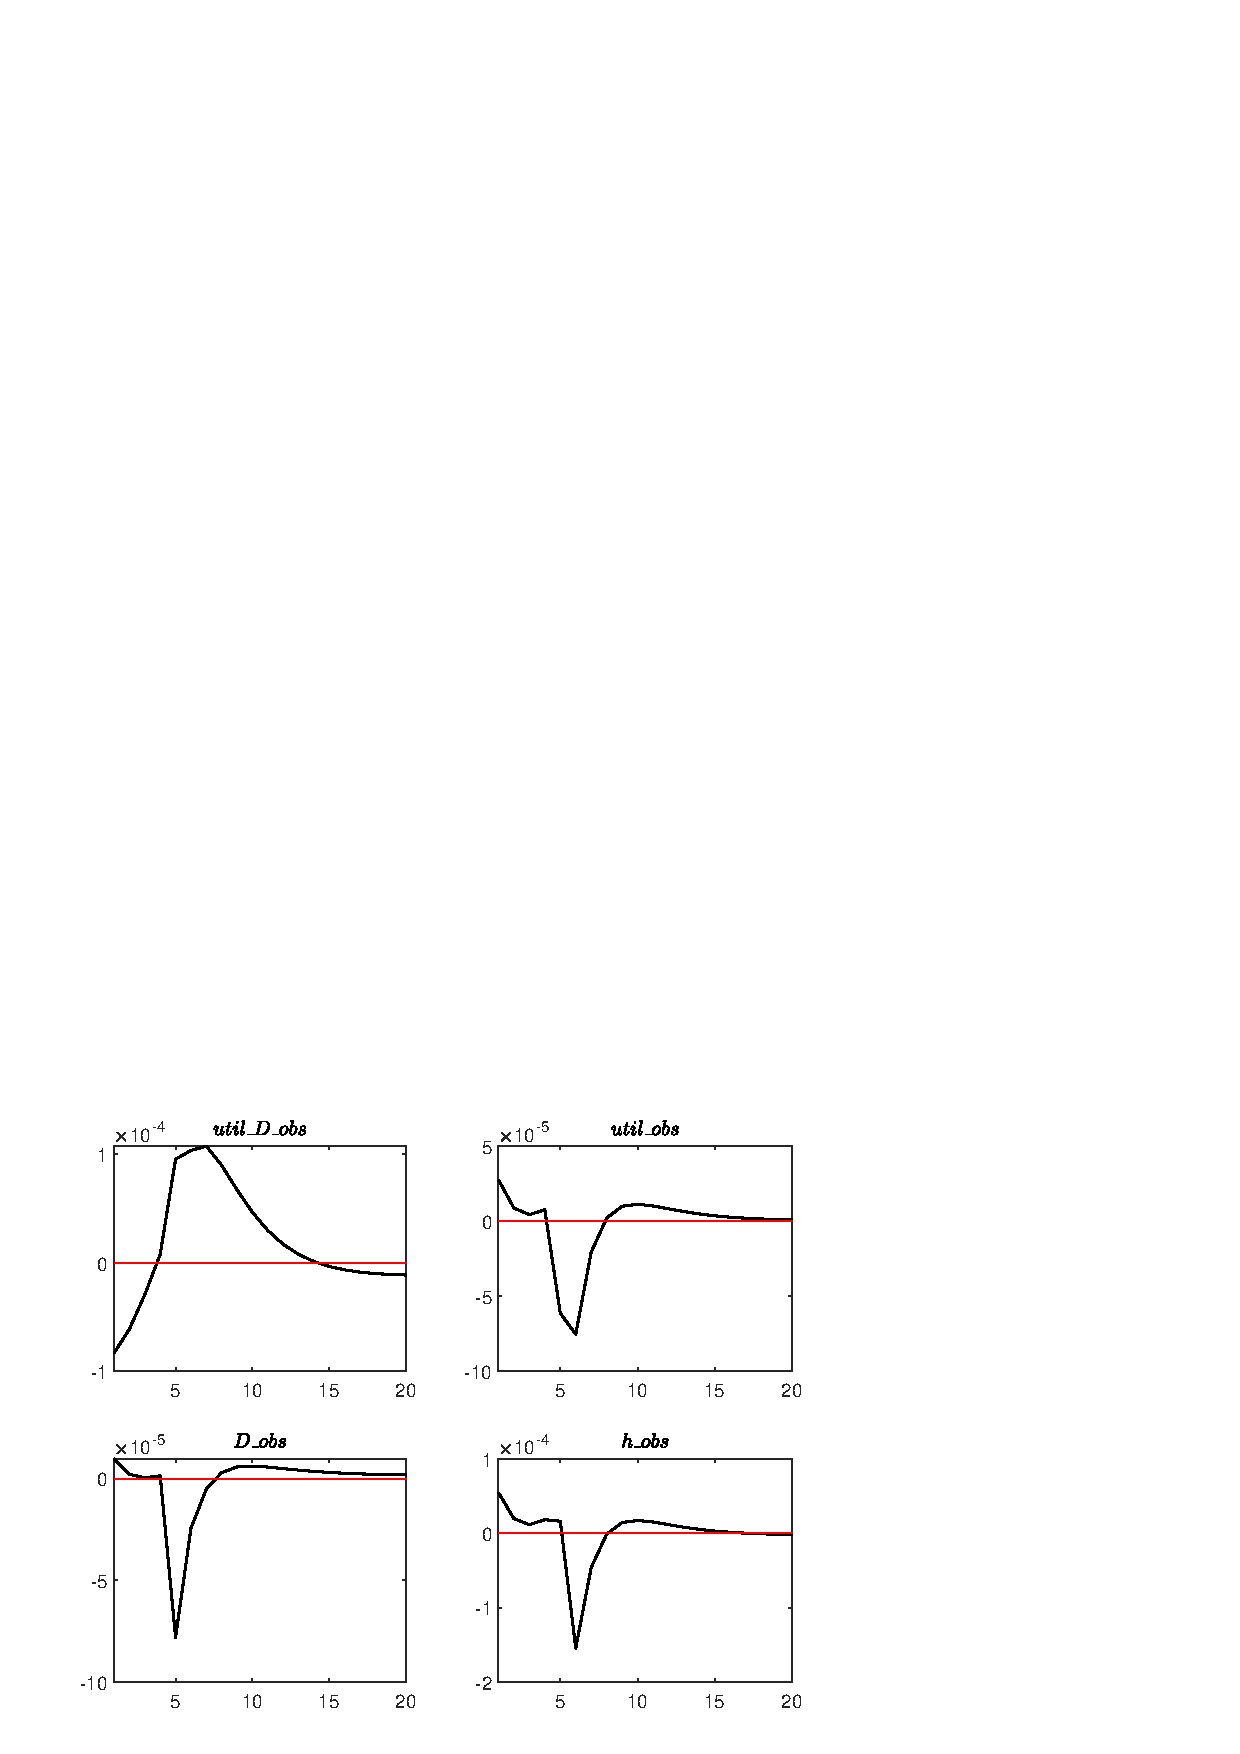
\includegraphics[width=0.80\textwidth]{BRS_sectoral/graphs/BRS_sectoral_IRF_e_muC_news2}
\caption{Impulse response functions (orthogonalized shock to ${e_{muC,-4}}$).}\label{Fig:IRF:e_muC_news:2}
\end{figure}
 
\begin{figure}[H]
\centering 
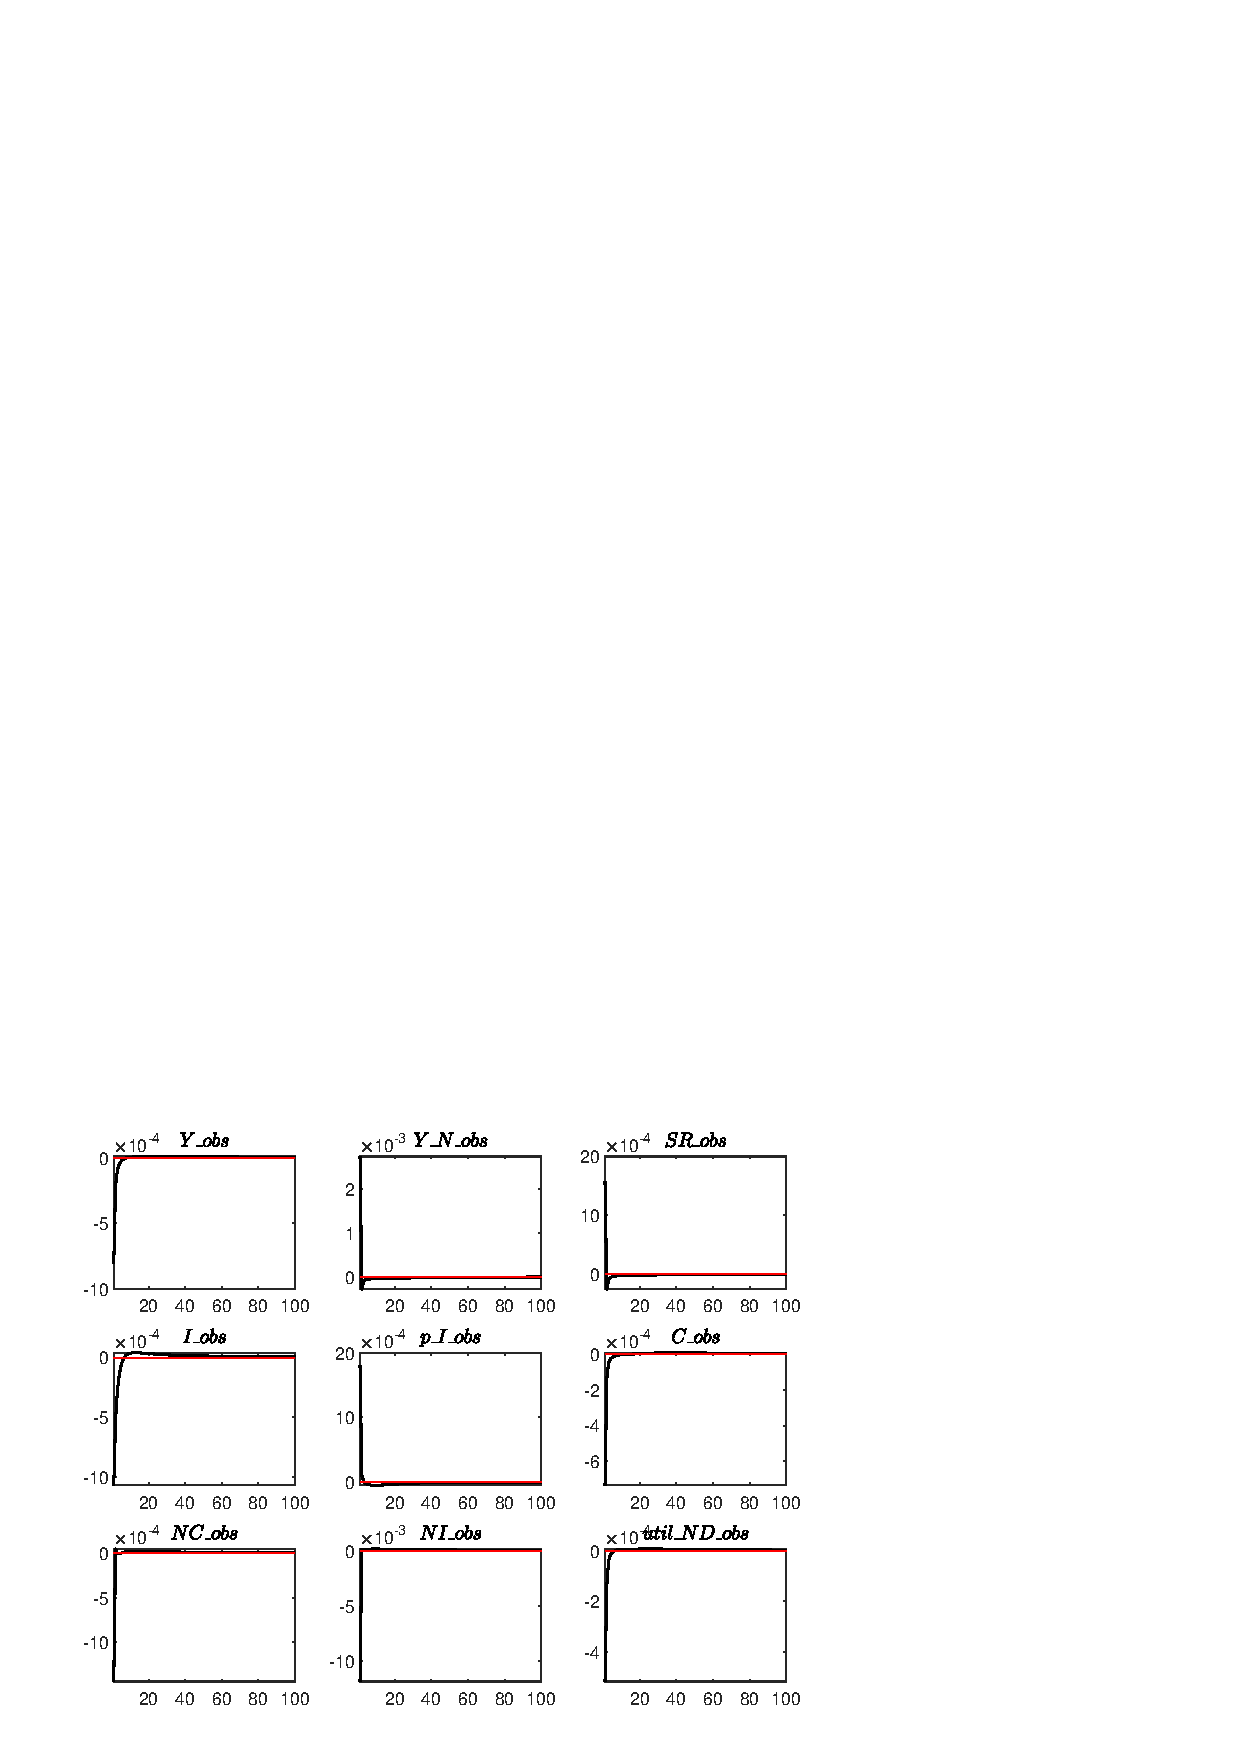
\includegraphics[width=0.80\textwidth]{BRS_sectoral/graphs/BRS_sectoral_IRF_e_muI1}
\caption{Impulse response functions (orthogonalized shock to ${e_{muI}}$).}\label{Fig:IRF:e_muI:1}
\end{figure}
 
\begin{figure}[H]
\centering 
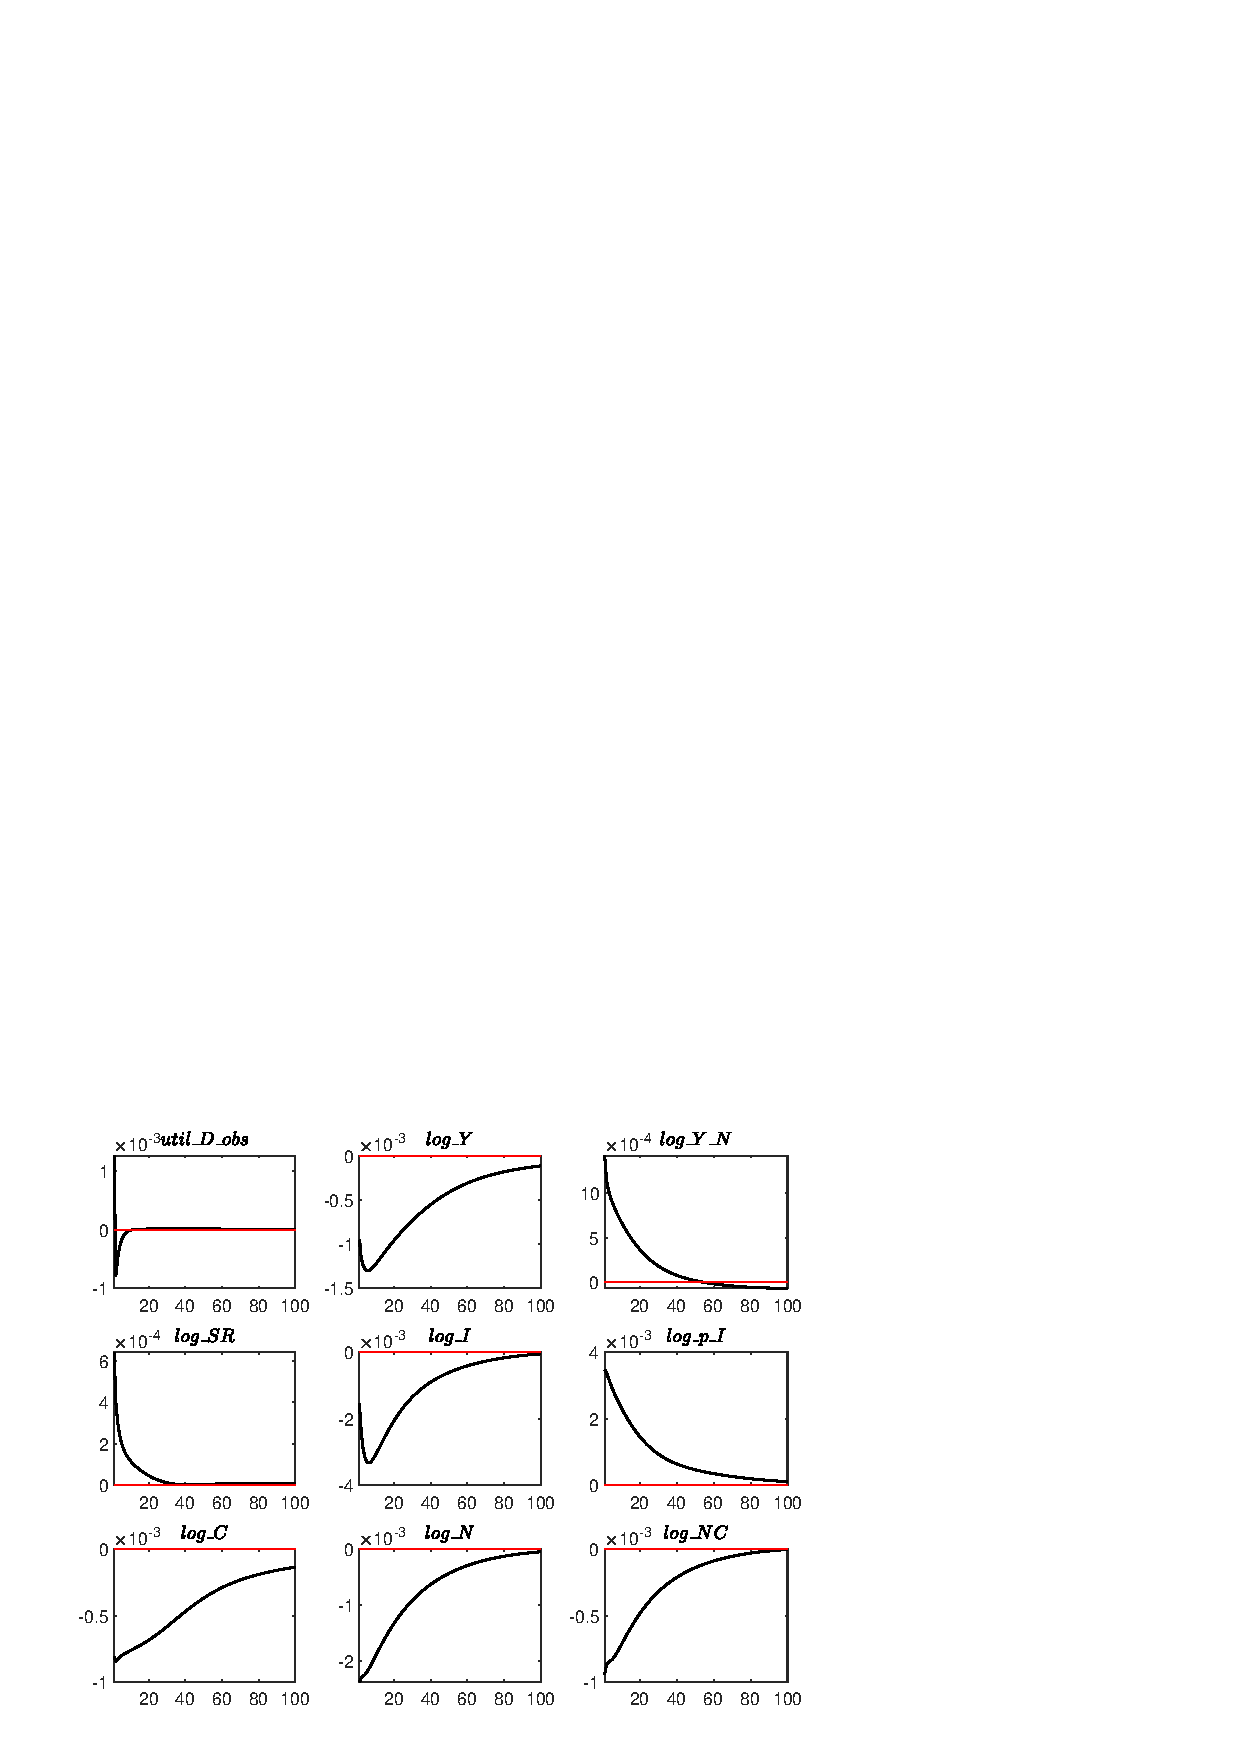
\includegraphics[width=0.80\textwidth]{BRS_sectoral/graphs/BRS_sectoral_IRF_e_muI2}
\caption{Impulse response functions (orthogonalized shock to ${e_{muI}}$).}\label{Fig:IRF:e_muI:2}
\end{figure}
 
\begin{figure}[H]
\centering 
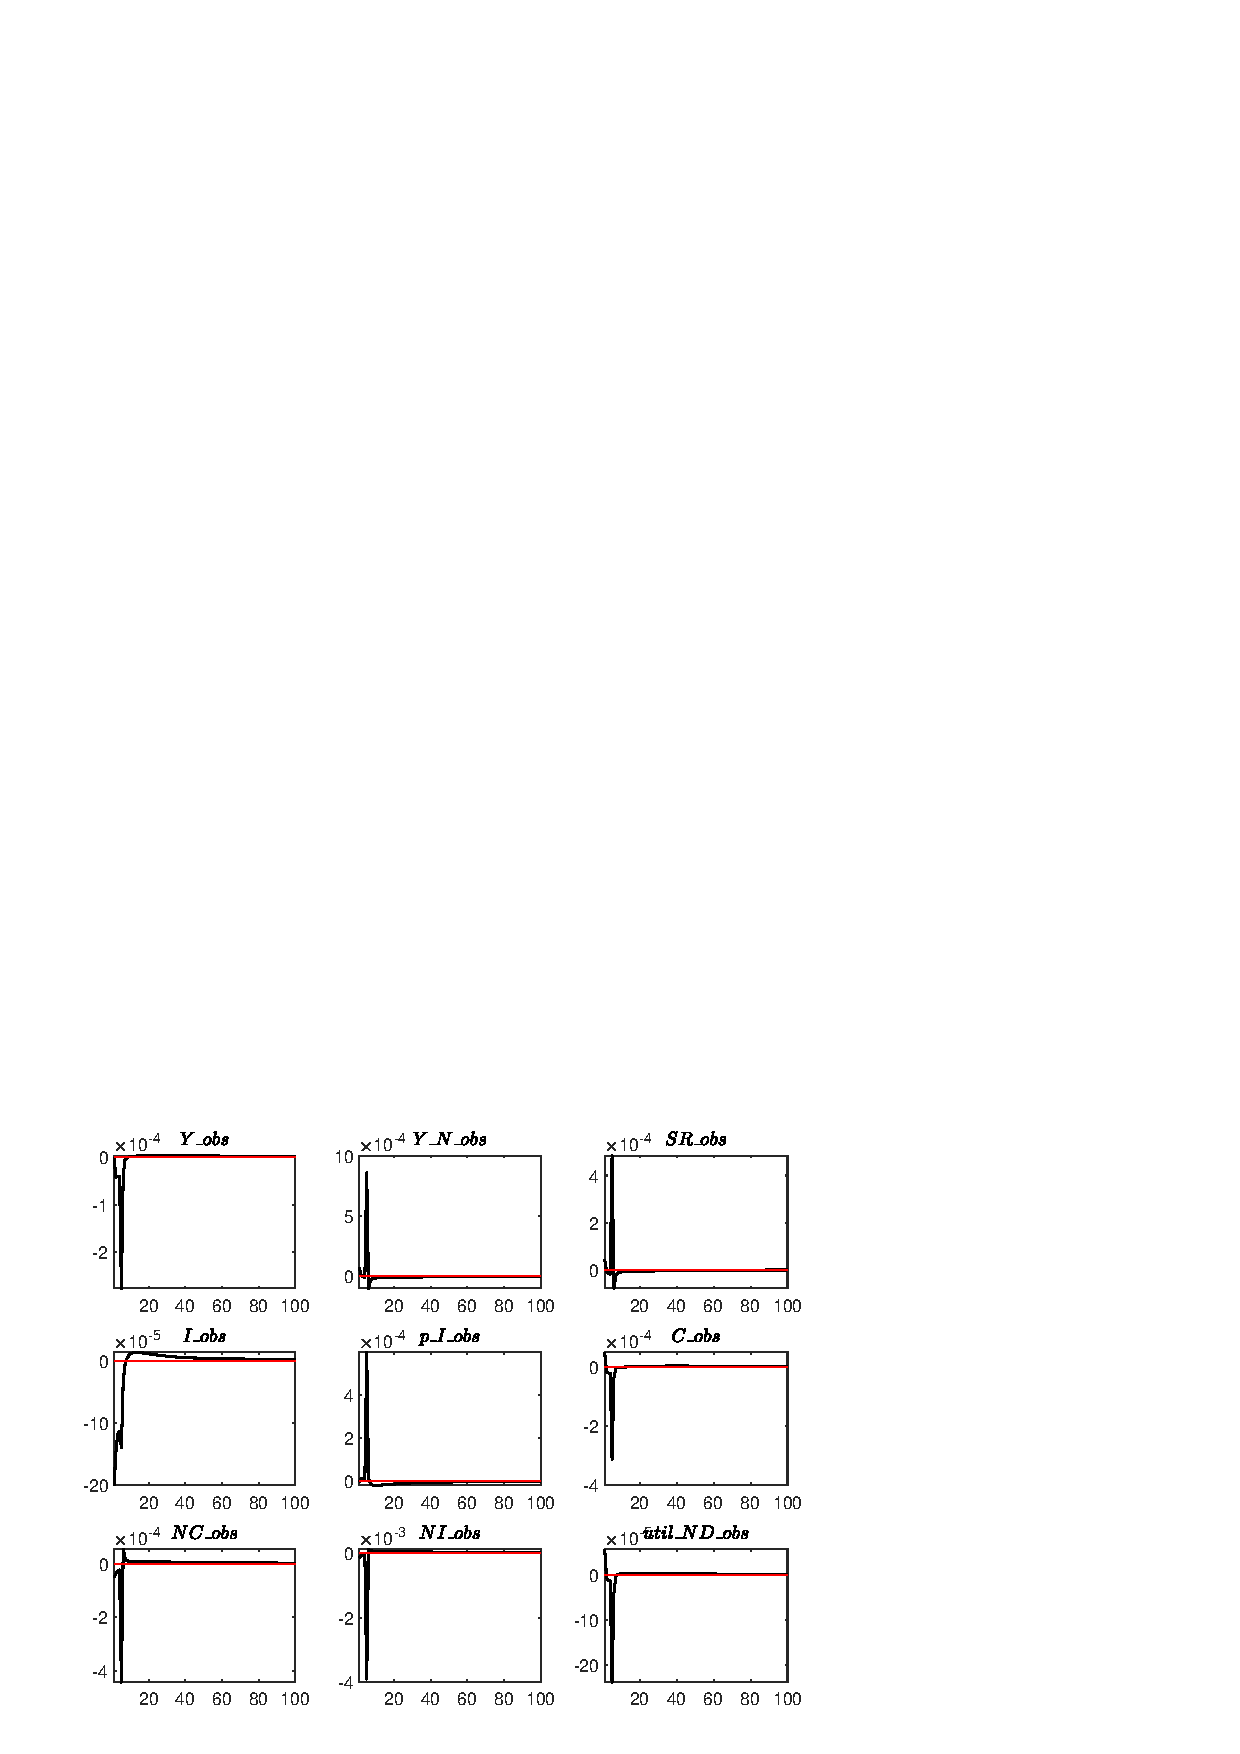
\includegraphics[width=0.80\textwidth]{BRS_sectoral/graphs/BRS_sectoral_IRF_e_muI_news1}
\caption{Impulse response functions (orthogonalized shock to ${e_{muI,-4}}$).}\label{Fig:IRF:e_muI_news:1}
\end{figure}
 
\begin{figure}[H]
\centering 
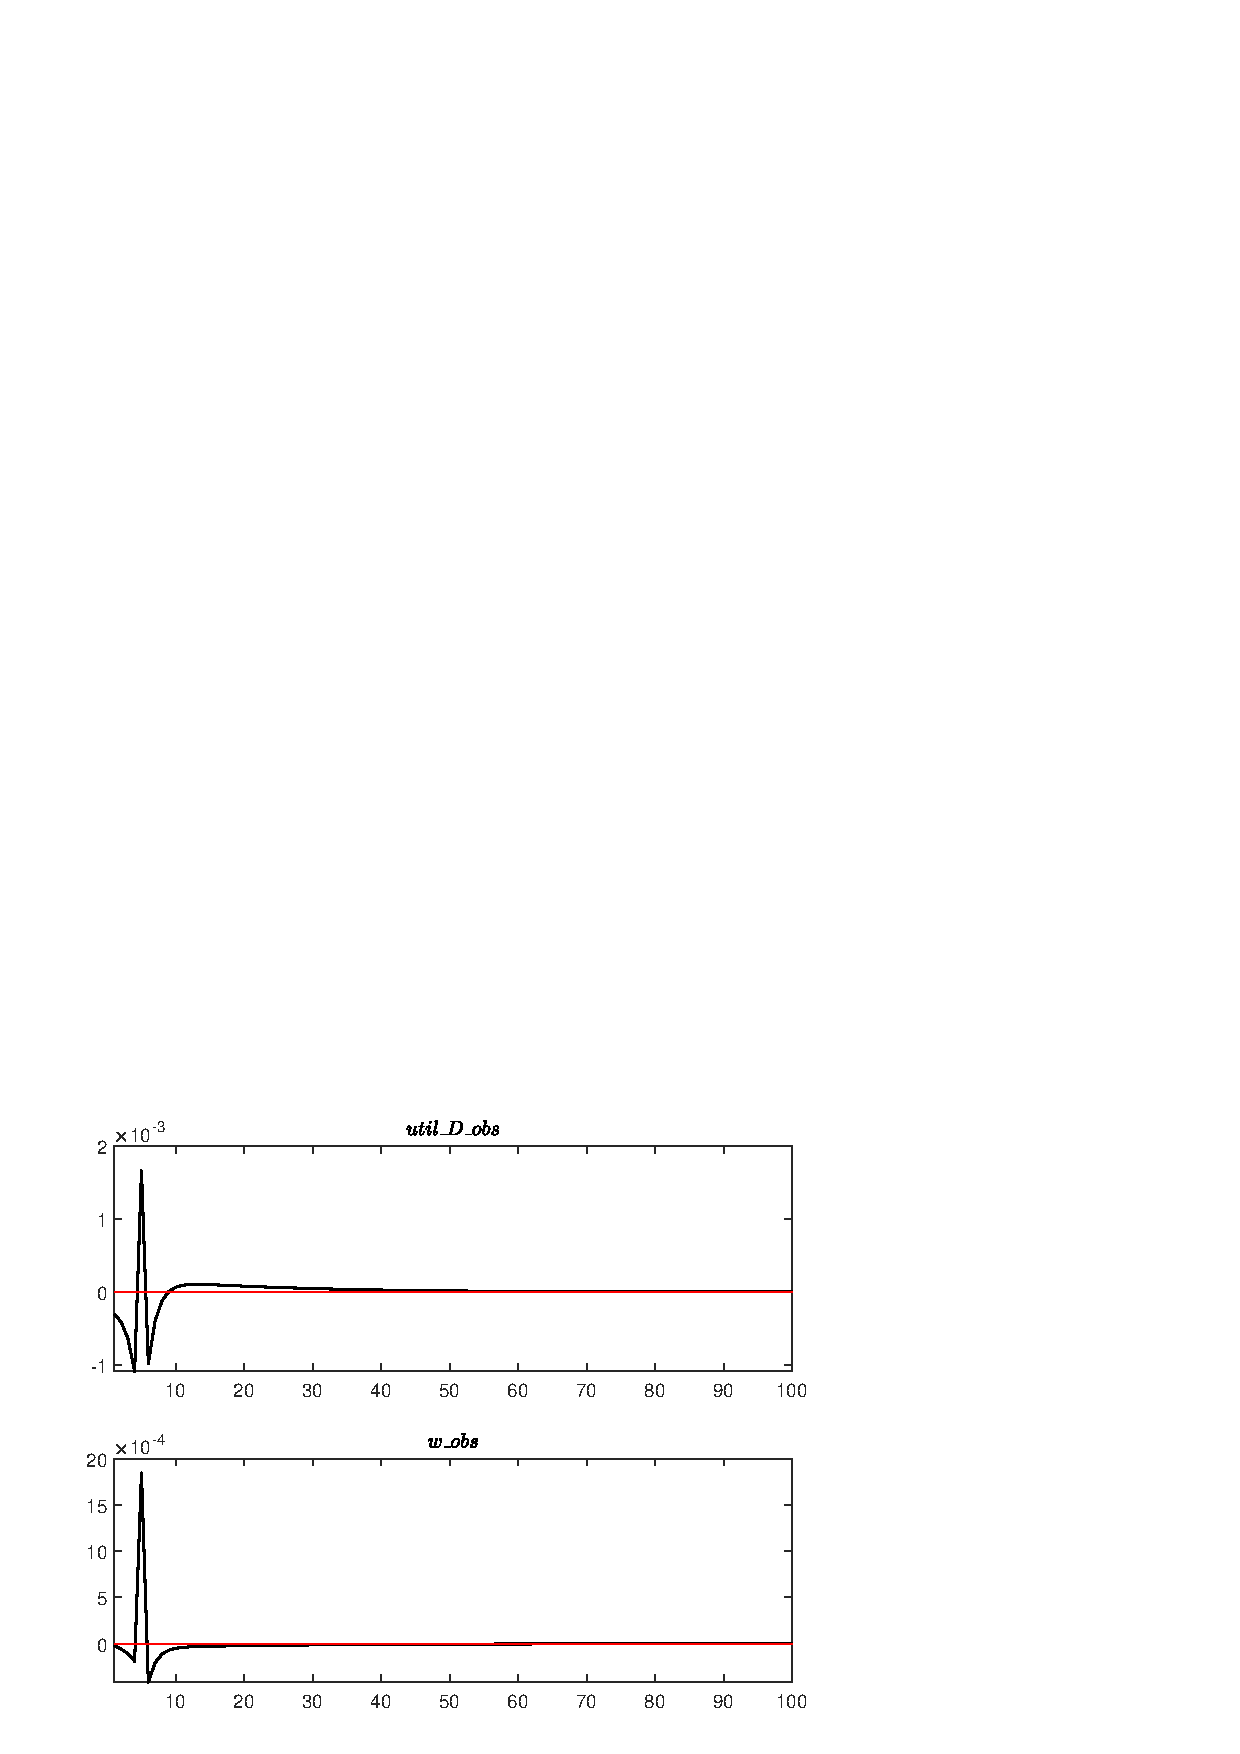
\includegraphics[width=0.80\textwidth]{BRS_sectoral/graphs/BRS_sectoral_IRF_e_muI_news2}
\caption{Impulse response functions (orthogonalized shock to ${e_{muI,-4}}$).}\label{Fig:IRF:e_muI_news:2}
\end{figure}
 
 
% End Of TeX file. 
